\documentclass{article}\usepackage{longtable}\usepackage{graphicx}\usepackage{array}\date{\today}\newcolumntype{L}[1]{>{\raggedright\let\newline\\\arraybackslash\hspace{0pt}}m{#1}}\newcolumntype{C}[1]{>{\let\newline\\\arraybackslash\hspace{0pt}}m{#1}}\newcolumntype{R}[1]{>{\raggedleft\let\newline\\\arraybackslash\hspace{0pt}}m{#1}}\setlength{\textwidth}{7.1in}\setlength{\oddsidemargin}{-0.4in}\setlength{\textheight}{9.6in}\setlength{\topmargin}{-0.8in}\begin{document}\today\section{Report of PCAWG objects}\tiny 

% latex table generated in R 3.6.3 by xtable 1.8-4 package
% Sat Jun 13 13:34:26 2020
\begin{longtable}{R{.2in}L{1in}L{.5in}R{.2in}R{.2in}L{1in}L{1in}R{1in}}
  \hline
 & Cancer\_type & Feature\_type & Number.of.samples & Number.of.features & Sum.of.features.for.group.1 & Sum.of.features.for.group.2 & sum\_all\_ct \\ 
  \hline
1 & Biliary-AdenoCA & nucleotidesubstitution1 & 15.00 & 6.00 & 31708, 10657, 95289, 23511, 85704, 11819 & 7148, 3094, 16771, 5196, 13878, 3056 & 1854.00 \\ 
  2 & Biliary-AdenoCA & nucleotidesubstitution3 & 15.00 & 96.00 & 1877, 1438, 227, 1624, 720, 496, 111, 921, 6704, 3153, 11597, 3308, 3069, 286... & 552, 369, 77, 411, 259, 164, 41, 240, 1336, 550, 1672, 651, 501, 428, 271, 73... & 1854.00 \\ 
  3 & Biliary-AdenoCA & signatures & 15.00 & 67.00 & 23265.3990159484, 6335.28556545343, 129.905521239188, 946.246316321856, 6246.... & 3278.11921199857, 1682.22358160167, 73.4372680276237, 183.531608209343, 681.7... & 1854.00 \\ 
  4 & Bladder-TCC & nucleotidesubstitution1 & 9.00 & 6.00 & 11247, 23297, 36661, 4894, 10328, 2397 & 4316, 8187, 15153, 1945, 3241, 1200 & 1854.00 \\ 
  5 & Bladder-TCC & nucleotidesubstitution3 & 9.00 & 96.00 & 864, 564, 138, 492, 364, 221, 59, 395, 1115, 570, 1678, 785, 463, 264, 301, 5... & 332, 238, 47, 213, 162, 71, 27, 164, 471, 225, 651, 282, 170, 110, 118, 263, ... & 1854.00 \\ 
  6 & Bladder-TCC & signatures & 9.00 & 67.00 & 3850.16917289413, 19223.2271315855, -1.91668633071992e-12, 1589.77619536001, ... & 1392.31651751711, 8469.72805991824, 114.147357111078, 420.570288846855, 1008.... & 1854.00 \\ 
  7 & Bone-Benign & nucleotidesubstitution1 & 5.00 & 6.00 & 485, 166, 954, 422, 375, 201 & 356, 109, 607, 260, 297, 150 & 1854.00 \\ 
  8 & Bone-Benign & nucleotidesubstitution3 & 5.00 & 96.00 & 65, 57, 11, 58, 18, 8, 6, 16, 99, 31, 123, 61, 32, 31, 34, 46, 53, 18, 32, 58... & 62, 40, 6, 33, 10, 4, 4, 5, 58, 26, 86, 41, 33, 16, 20, 23, 53, 9, 23, 36, 10... & 1854.00 \\ 
  9 & Bone-Benign & signatures & 5.00 & 67.00 & 272.633178022064, 6.8949703243094, 4.25411415211175e-13, -5.7362876998306e-13... & 185.900784176247, 18.3022252942639, 20.3498574229508, 10.5184717476863, 38.64... & 1854.00 \\ 
  10 & Bone-Epith & nucleotidesubstitution1 & 6.00 & 6.00 & 2055, 1675, 4598, 1603, 2404, 899 & 752, 432, 1403, 608, 1010, 555 & 1854.00 \\ 
  11 & Bone-Epith & nucleotidesubstitution3 & 6.00 & 96.00 & 218, 176, 22, 182, 94, 58, 18, 96, 270, 130, 489, 158, 173, 98, 97, 168, 289,... & 82, 66, 10, 57, 36, 27, 5, 38, 91, 50, 126, 77, 75, 47, 45, 67, 92, 35, 41, 1... & 1854.00 \\ 
  12 & Bone-Epith & signatures & 6.00 & 67.00 & 1115.38625439732, 1256.17947460705, 338.427340519909, 4.47761830220823e-13, 5... & 254.257374881263, 172.048594645656, 237.956131105912, 2.14435506428417, 29.52... & 1854.00 \\ 
  13 & Bone-Osteosarc & nucleotidesubstitution1 & 27.00 & 6.00 & 16765, 11412, 24999, 12860, 16676, 8919 & 6890, 4496, 10281, 4750, 6866, 3728 & 1854.00 \\ 
  14 & Bone-Osteosarc & nucleotidesubstitution3 & 27.00 & 96.00 & 1686, 1259, 225, 1467, 858, 481, 164, 894, 2018, 1048, 1810, 1357, 801, 518, ... & 673, 433, 78, 546, 353, 189, 97, 331, 746, 368, 576, 574, 306, 217, 213, 406,... & 1854.00 \\ 
  15 & Bone-Osteosarc & signatures & 27.00 & 67.00 & 3087.16399731988, 2747.55749753469, 4560.40299034362, 28.6361005032861, 728.8... & 827.166228306351, 1412.52387935667, 597.641686142282, 63.8685867690686, 93.61... & 1854.00 \\ 
  16 & Breast-AdenoCA & nucleotidesubstitution1 & 136.00 & 6.00 & 102333, 109936, 197258, 62235, 79343, 40654 & 56188, 77621, 126098, 33510, 43220, 25667 & 1854.00 \\ 
  17 & Breast-AdenoCA & nucleotidesubstitution3 & 136.00 & 96.00 & 9831, 7910, 1287, 7413, 5454, 3377, 1368, 5709, 9906, 5161, 15766, 7683, 4141... & 5028, 3863, 594, 3756, 3149, 1902, 812, 3180, 5323, 2514, 6708, 4021, 2353, 1... & 1854.00 \\ 
  18 & Breast-AdenoCA & signatures & 136.00 & 67.00 & 33782.5073769357, 60519.3153150691, 43994.423064049, 1057.49110358632, 24947.... & 13063.7562425675, 59489.4923173392, 19659.484697551, 1061.102147616, 3989.171... & 1854.00 \\ 
  19 & Breast-DCIS & nucleotidesubstitution1 & 2.00 & 6.00 & 546, 225, 1193, 351, 558, 213 & 233, 96, 431, 121, 188, 88 & 1854.00 \\ 
  20 & Breast-DCIS & nucleotidesubstitution3 & 2.00 & 96.00 & 48, 53, 8, 40, 17, 16, 7, 14, 60, 44, 142, 50, 26, 33, 33, 45, 80, 37, 39, 80... & 36, 21, 6, 18, 9, 7, 2, 6, 25, 13, 51, 21, 6, 10, 11, 10, 20, 9, 12, 19, 2, 0... & 1854.00 \\ 
  21 & Breast-DCIS & signatures & 2.00 & 67.00 & 315.928195789719, 97.2931650999246, 202.647807661729, -3.04916636196287e-13, ... & 110.640043875143, 18.2712544543606, 76.2233628074865, 35.6127566134672, 87.19... & 1854.00 \\ 
  22 & Breast-LobularCA & nucleotidesubstitution1 & 8.00 & 6.00 & 5483, 16385, 27590, 1577, 2558, 899 & 2009, 7298, 8956, 605, 848, 374 & 1854.00 \\ 
  23 & Breast-LobularCA & nucleotidesubstitution3 & 8.00 & 96.00 & 288, 205, 43, 185, 157, 85, 37, 165, 471, 210, 841, 245, 129, 141, 128, 172, ... & 115, 82, 18, 56, 77, 44, 20, 77, 162, 73, 246, 95, 48, 53, 52, 52, 97, 41, 66... & 1854.00 \\ 
  24 & Breast-LobularCA & signatures & 8.00 & 67.00 & 1967.44457663833, 21139.0955080961, 4.34132834781002, 14.5210517100428, 2177.... & 567.884677256106, 6786.17183874461, 42.0353641258717, 13.5266998020772, 184.3... & 1854.00 \\ 
  25 & Cervix-AdenoCA & nucleotidesubstitution1 & 2.00 & 6.00 & 1004, 676, 3594, 372, 688, 200 & 268, 113, 825, 143, 208, 88 & 1854.00 \\ 
  26 & Cervix-AdenoCA & nucleotidesubstitution3 & 2.00 & 96.00 & 102, 55, 12, 55, 16, 21, 12, 17, 108, 59, 502, 96, 29, 23, 17, 64, 72, 33, 44... & 19, 15, 4, 15, 8, 4, 4, 6, 33, 14, 130, 21, 6, 10, 9, 17, 24, 11, 9, 11, 5, 1... & 1854.00 \\ 
  27 & Cervix-AdenoCA & signatures & 2.00 & 67.00 & 1183.27611742386, 1015.81065139978, -1.28021207936864e-12, 3.08837207692665e-... & 300.957653425067, 86.53603935672, -1.89404968212677e-13, -9.54024491611131e-1... & 1854.00 \\ 
  28 & Cervix-SCC & nucleotidesubstitution1 & 16.00 & 6.00 & 9432, 16150, 33724, 4204, 6292, 2374 & 3942, 9697, 15700, 1838, 2612, 1041 & 1854.00 \\ 
  29 & Cervix-SCC & nucleotidesubstitution3 & 16.00 & 96.00 & 791, 454, 111, 520, 327, 190, 118, 340, 1014, 564, 2700, 739, 312, 258, 267, ... & 259, 170, 36, 206, 202, 91, 43, 171, 400, 213, 857, 281, 140, 108, 117, 257, ... & 1854.00 \\ 
  30 & Cervix-SCC & signatures & 16.00 & 67.00 & 6003.54063689202, 15679.5768912425, 120.462065300687, 25.5812161351638, 2470.... & 1924.32211718459, 9137.67604748009, 81.5275955273514, 54.0575534644598, 479.4... & 1854.00 \\ 
  31 & CNS-GBM & nucleotidesubstitution1 & 34.00 & 6.00 & 24392, 12080, 79747, 20246, 28954, 8645 & 11416, 5690, 193921, 8988, 14027, 3817 & 1854.00 \\ 
  32 & CNS-GBM & nucleotidesubstitution3 & 34.00 & 96.00 & 2878, 2463, 328, 2645, 1369, 693, 179, 1405, 3909, 1791, 22569, 2682, 1507, 9... & 1210, 1037, 127, 1124, 612, 375, 90, 599, 6154, 20738, 7011, 16245, 681, 397,... & 1854.00 \\ 
  33 & CNS-GBM & signatures & 34.00 & 67.00 & 53722.395685486, 982.274782199956, 8032.54943302977, -2.59674061573124e-11, 1... & 14233.9627236758, 5137.78331043576, 3210.2869595515, 99.484600875727, 289.604... & 1854.00 \\ 
  34 & CNS-Medullo & nucleotidesubstitution1 & 106.00 & 6.00 & 17235, 7311, 40746, 9389, 15202, 4779 & 9973, 5020, 20581, 5755, 9501, 3105 & 1854.00 \\ 
  35 & CNS-Medullo & nucleotidesubstitution3 & 106.00 & 96.00 & 1729, 1378, 217, 1191, 1028, 577, 209, 802, 2179, 1188, 8132, 1614, 677, 477,... & 1062, 727, 125, 664, 743, 387, 133, 548, 1269, 657, 3529, 893, 450, 294, 312,... & 1854.00 \\ 
  36 & CNS-Medullo & signatures & 106.00 & 67.00 & 19473.4736075548, 604.483949094173, 1174.13623059921, 264.081637984501, 845.4... & 8167.9353243652, 351.807681861559, 248.026445823009, 298.193494944641, 776.80... & 1854.00 \\ 
  37 & CNS-Oligo & nucleotidesubstitution1 & 15.00 & 6.00 & 3097, 1842, 11182, 2674, 6622, 1490 & 1539, 823, 5875, 1215, 3065, 694 & 1854.00 \\ 
  38 & CNS-Oligo & nucleotidesubstitution3 & 15.00 & 96.00 & 415, 347, 51, 350, 224, 132, 17, 226, 575, 299, 2161, 430, 268, 159, 167, 260... & 197, 157, 23, 165, 94, 66, 11, 86, 325, 158, 1079, 212, 129, 86, 75, 120, 357... & 1854.00 \\ 
  39 & CNS-Oligo & signatures & 15.00 & 67.00 & 5126.88905736351, 103.634612189594, 13.2265522430431, -3.02190816308251e-12, ... & 2560.34978285385, 103.382209507906, 143.422630394916, 6.5587090968034e-13, 26... & 1854.00 \\ 
  40 & CNS-PiloAstro & nucleotidesubstitution1 & 42.00 & 6.00 & 693, 312, 2514, 503, 1005, 257 & 1000, 414, 2941, 753, 1281, 372 & 1854.00 \\ 
  41 & CNS-PiloAstro & nucleotidesubstitution3 & 42.00 & 96.00 & 75, 72, 12, 61, 36, 15, 17, 38, 162, 59, 523, 86, 44, 29, 30, 53, 126, 42, 77... & 130, 97, 17, 109, 47, 23, 13, 33, 161, 91, 416, 104, 69, 38, 64, 69, 174, 67,... & 1854.00 \\ 
  42 & CNS-PiloAstro & signatures & 42.00 & 67.00 & 1258.98674348096, 55.6489881974731, 19.4888084531813, 11.1663101349811, 44.09... & 931.474566961833, 71.7328520114922, 69.5203805748062, 66.0956734122494, 106.7... & 1854.00 \\ 
  43 & ColoRect-AdenoCA & nucleotidesubstitution1 & 37.00 & 6.00 & 1065268, 26616, 656012, 71060, 320700, 595450 & 1137079, 19165, 561617, 67491, 399462, 780714 & 1854.00 \\ 
  44 & ColoRect-AdenoCA & nucleotidesubstitution3 & 37.00 & 96.00 & 12072, 10664, 1091, 27438, 3059, 1638, 280, 3024, 10598, 11158, 46824, 17602,... & 6698, 7115, 733, 34697, 2233, 1236, 210, 2260, 8038, 10211, 24502, 16972, 367... & 1854.00 \\ 
  45 & ColoRect-AdenoCA & signatures & 37.00 & 67.00 & 65329.7620929798, 7900.78680597273, 2.1501559835312e-10, -3.54528434780563e-1... & 13702.1023818585, 8131.52084664726, 1.55350268244454e-10, 71.26650177996, 215... & 1854.00 \\ 
  46 & Eso-AdenoCA & nucleotidesubstitution1 & 65.00 & 6.00 & 127271, 51688, 202501, 100316, 221397, 349514 & 77347, 38979, 131812, 56101, 106263, 153940 & 1854.00 \\ 
  47 & Eso-AdenoCA & nucleotidesubstitution3 & 65.00 & 96.00 & 12213, 6829, 1072, 7239, 3777, 2321, 666, 4229, 10636, 5701, 26110, 8157, 471... & 7428, 4222, 678, 4628, 2558, 1506, 565, 2792, 7136, 3661, 14430, 5451, 2889, ... & 1854.00 \\ 
  48 & Eso-AdenoCA & signatures & 65.00 & 67.00 & 54680.9888833264, 21050.9584386567, 523.758528548971, 2.66176731934127e-11, 1... & 29457.2957528153, 20674.7117826262, 343.427202505903, 438.520377777157, 11258... & 1854.00 \\ 
  49 & Head-SCC & nucleotidesubstitution1 & 32.00 & 6.00 & 54802, 83020, 140484, 27094, 35653, 14709 & 16784, 28222, 49282, 8665, 11900, 5878 & 1854.00 \\ 
  50 & Head-SCC & nucleotidesubstitution3 & 32.00 & 96.00 & 4530, 2608, 624, 2758, 2022, 1115, 423, 2323, 4300, 2555, 6562, 3355, 2522, 1... & 1350, 740, 156, 856, 731, 368, 154, 766, 1516, 816, 2432, 1092, 672, 465, 488... & 1854.00 \\ 
  51 & Head-SCC & signatures & 32.00 & 67.00 & 12852.6025869812, 70367.6842496578, 1162.92795400683, 9415.69828177657, 5394.... & 4914.08924169728, 25658.0598087451, 1909.5969787338, 277.065628628594, 863.52... & 1854.00 \\ 
  52 & Kidney-ChRCC & nucleotidesubstitution1 & 38.00 & 6.00 & 6581, 3953, 14153, 3943, 5683, 3241 & 5919, 2983, 13429, 3550, 4943, 3255 & 1854.00 \\ 
  53 & Kidney-ChRCC & nucleotidesubstitution3 & 38.00 & 96.00 & 941, 568, 108, 544, 307, 183, 59, 351, 810, 432, 2343, 561, 387, 255, 324, 34... & 872, 474, 91, 451, 265, 143, 63, 242, 646, 387, 2503, 527, 317, 204, 283, 338... & 1854.00 \\ 
  54 & Kidney-ChRCC & signatures & 38.00 & 67.00 & 5436.00747142877, 868.310797854879, 2257.51006804321, 405.375430232798, 1447.... & 5801.31310937803, 562.828739474715, 1274.17896218364, 342.238552568846, 239.0... & 1854.00 \\ 
  55 & Kidney-RCC.clearcell & nucleotidesubstitution1 & 86.00 & 6.00 & 79755, 43304, 106472, 93346, 69569, 39892 & 29211, 14817, 40284, 29463, 21734, 11075 & 1854.00 \\ 
  56 & Kidney-RCC.clearcell & nucleotidesubstitution3 & 86.00 & 96.00 & 9873, 4933, 1070, 5318, 3956, 2630, 722, 4441, 7904, 4520, 8295, 6406, 7872, ... & 3989, 1822, 397, 1877, 1589, 911, 262, 1330, 2782, 1594, 3738, 2163, 2657, 92... & 1854.00 \\ 
  57 & Kidney-RCC.clearcell & signatures & 86.00 & 67.00 & 18037.301938108, 1859.36714201358, 3322.64219011167, 8736.01316433894, 1610.0... & 7652.78267084567, 1212.98036888003, 3366.19193324173, 3340.12514261013, 657.2... & 1854.00 \\ 
  58 & Kidney-RCC.papillary & nucleotidesubstitution1 & 30.00 & 6.00 & 21259, 15798, 32767, 20276, 25892, 17065 & 5429, 3703, 9593, 3912, 5751, 3014 & 1854.00 \\ 
  59 & Kidney-RCC.papillary & nucleotidesubstitution3 & 30.00 & 96.00 & 2256, 1236, 271, 1451, 1168, 961, 226, 1709, 2528, 1436, 2078, 2098, 1497, 76... & 540, 375, 83, 372, 298, 185, 64, 333, 664, 379, 903, 490, 345, 191, 246, 420,... & 1854.00 \\ 
  60 & Kidney-RCC.papillary & signatures & 30.00 & 67.00 & 4450.63124050123, 1337.95044141494, 1068.26319467467, 88.4020408682784, 1587.... & 1946.11317569171, 1157.42022224246, 1721.58680884854, 295.9611456123, 652.017... & 1854.00 \\ 
  61 & Liver-HCC & nucleotidesubstitution1 & 207.00 & 6.00 & 378482, 133729, 448007, 278339, 667430, 122636 & 116079, 44796, 133375, 97596, 165501, 39011 & 1854.00 \\ 
  62 & Liver-HCC & nucleotidesubstitution3 & 207.00 & 96.00 & 37099, 24969, 5957, 23315, 10684, 6613, 1783, 12345, 34022, 17850, 22428, 229... & 10462, 7819, 1454, 6986, 3639, 2351, 576, 3958, 9841, 5363, 6308, 6741, 8521,... & 1854.00 \\ 
  63 & Liver-HCC & signatures & 207.00 & 67.00 & 34177.371610163, 18599.0562281778, 62433.0776275653, 118296.61969812, 41964.3... & 8729.27361090133, 6816.00758221106, 31888.0223328352, 27777.0103900263, 8361.... & 1854.00 \\ 
  64 & Lung-AdenoCA & nucleotidesubstitution1 & 17.00 & 6.00 & 84217, 27462, 50984, 25766, 23707, 11368 & 23204, 15133, 33878, 9522, 12162, 12953 & 1854.00 \\ 
  65 & Lung-AdenoCA & nucleotidesubstitution3 & 17.00 & 96.00 & 7623, 4791, 1693, 4989, 1923, 917, 324, 1498, 3211, 1485, 2606, 1884, 1955, 9... & 2051, 1366, 381, 1311, 620, 323, 118, 577, 1362, 665, 1437, 844, 641, 416, 63... & 1854.00 \\ 
  66 & Lung-AdenoCA & signatures & 17.00 & 67.00 & 4312.76857351021, 12521.5487518205, 2413.42502332668, 79924.9564211879, 2827.... & 2589.91088098383, 17309.0676984335, 641.041891128399, 14960.2794380372, 571.7... & 1854.00 \\ 
  67 & Lung-SCC & nucleotidesubstitution1 & 34.00 & 6.00 & 341617, 141834, 207863, 124123, 146834, 37810 & 67052, 44446, 62665, 27885, 32664, 12340 & 1854.00 \\ 
  68 & Lung-SCC & nucleotidesubstitution3 & 34.00 & 96.00 & 31727, 18373, 7165, 19728, 10174, 4630, 2163, 7524, 14965, 7038, 6918, 9240, ... & 6160, 3990, 1170, 3878, 2333, 1193, 666, 2000, 3576, 1723, 2440, 2432, 2148, ... & 1854.00 \\ 
  69 & Lung-SCC & signatures & 34.00 & 67.00 & 5284.47432801545, 46408.5174776554, 2258.80965858908, 307368.801840694, 3355.... & 3590.42247514167, 21008.3669518586, 5515.57210401424, 44482.5695998976, 1180.... & 1854.00 \\ 
  70 & Lymph-BNHL & nucleotidesubstitution1 & 51.00 & 6.00 & 45838, 21361, 92833, 43857, 76409, 80569 & 10010, 4779, 20653, 10960, 19033, 19129 & 1854.00 \\ 
  71 & Lymph-BNHL & nucleotidesubstitution3 & 51.00 & 96.00 & 4090, 3325, 412, 3205, 2360, 1233, 299, 2445, 7049, 3549, 9542, 4917, 4143, 2... & 913, 735, 97, 657, 471, 292, 74, 553, 1553, 863, 1639, 1010, 1033, 546, 559, ... & 1854.00 \\ 
  72 & Lymph-BNHL & signatures & 51.00 & 67.00 & 18968.4128354178, 3098.80254257847, 1397.1840786762, 28.2888485268797, 22488.... & 2785.47138408916, 862.122022449951, 610.345507879906, 49.9955044491976, 1793.... & 1854.00 \\ 
  73 & Lymph-CLL & nucleotidesubstitution1 & 53.00 & 6.00 & 13002, 5129, 26586, 11620, 18434, 9829 & 7525, 3062, 15659, 7591, 9861, 3133 & 1854.00 \\ 
  74 & Lymph-CLL & nucleotidesubstitution3 & 53.00 & 96.00 & 1425, 1067, 198, 1051, 596, 370, 83, 479, 1796, 1103, 3699, 1265, 1098, 879, ... & 1072, 663, 137, 588, 372, 244, 46, 277, 1103, 617, 1906, 733, 753, 605, 728, ... & 1854.00 \\ 
  75 & Lymph-CLL & signatures & 53.00 & 67.00 & 8102.31966354739, 313.243843604807, 1182.21871202236, 82.7231197032934, 6337.... & 3933.20507477098, 227.929116280559, 1205.05344424519, 72.5071139182542, 3504.... & 1854.00 \\ 
  76 & Myeloid-AML & nucleotidesubstitution1 & 8.00 & 6.00 & 1155, 476, 3776, 711, 1215, 335 & 1019, 225, 1789, 453, 643, 187 & 1854.00 \\ 
  77 & Myeloid-AML & nucleotidesubstitution3 & 8.00 & 96.00 & 112, 83, 9, 70, 73, 12, 8, 36, 236, 149, 488, 185, 48, 55, 42, 64, 146, 39, 1... & 92, 49, 8, 47, 34, 19, 9, 27, 73, 46, 291, 59, 25, 17, 20, 44, 61, 32, 35, 51... & 1854.00 \\ 
  78 & Myeloid-AML & signatures & 8.00 & 67.00 & 1129.92868512001, 0.603188983673472, 7.13867893825946e-14, 0.336934260591716,... & 662.487131925736, 22.0891660067274, 4.61015669083346e-13, 5.20988757147899, -... & 1854.00 \\ 
  79 & Myeloid-MPN & nucleotidesubstitution1 & 19.00 & 6.00 & 1287, 772, 6189, 1004, 2022, 665 & 1603, 805, 5436, 1386, 2189, 969 & 1854.00 \\ 
  80 & Myeloid-MPN & nucleotidesubstitution3 & 19.00 & 96.00 & 201, 100, 10, 90, 116, 57, 16, 75, 450, 260, 933, 349, 106, 103, 88, 92, 260,... & 242, 136, 18, 104, 140, 55, 22, 93, 375, 193, 906, 296, 149, 125, 93, 152, 24... & 1854.00 \\ 
  81 & Myeloid-MPN & signatures & 19.00 & 67.00 & 2103.14910923093, 24.2170896216592, 121.199546585739, 17.0471777353132, 848.4... & 2013.05853307215, 45.7030081327688, 72.3441766702624, 13.3393319033685, 393.8... & 1854.00 \\ 
  82 & Ovary-AdenoCA & nucleotidesubstitution1 & 97.00 & 6.00 & 124081, 92075, 163415, 88479, 111234, 49316 & 45375, 38371, 56995, 33963, 41794, 19838 & 1854.00 \\ 
  83 & Ovary-AdenoCA & nucleotidesubstitution3 & 97.00 & 96.00 & 14043, 11390, 1631, 10718, 7887, 4246, 1832, 7817, 12059, 6450, 15797, 10581,... & 4822, 4137, 577, 3804, 3074, 1739, 958, 2947, 4213, 2173, 4579, 3941, 2027, 1... & 1854.00 \\ 
  84 & Ovary-AdenoCA & signatures & 97.00 & 67.00 & 31749.7656822093, 9336.00003639141, 77246.0741436906, 2269.770205119, 44988.0... & 8299.34309868655, 5859.61884300338, 21140.5279266568, 1157.67415422567, 9498.... & 1854.00 \\ 
  85 & Panc-AdenoCA & nucleotidesubstitution1 & 193.00 & 6.00 & 136960, 72755, 339695, 94677, 136853, 63302 & 78308, 43746, 155856, 52446, 82252, 46313 & 1854.00 \\ 
  86 & Panc-AdenoCA & nucleotidesubstitution3 & 193.00 & 96.00 & 13506, 11403, 1449, 9670, 5041, 3165, 836, 5252, 16041, 8327, 57744, 11566, 7... & 7380, 5309, 791, 5202, 3133, 1867, 667, 3139, 7973, 3920, 20678, 5835, 3701, ... & 1854.00 \\ 
  87 & Panc-AdenoCA & signatures & 193.00 & 67.00 & 139626.405073023, 28924.6063549603, 26290.3828812139, 1111.19622954746, 51889... & 46978.956887415, 21905.9459294641, 12084.2279285786, 1253.59627675103, 12516.... & 1854.00 \\ 
  88 & Panc-Endocrine & nucleotidesubstitution1 & 70.00 & 6.00 & 30379, 10745, 37445, 13098, 20270, 6537 & 35736, 10295, 35019, 11689, 16568, 5258 & 1854.00 \\ 
  89 & Panc-Endocrine & nucleotidesubstitution3 & 70.00 & 96.00 & 2376, 1660, 249, 1656, 852, 603, 137, 832, 2478, 1441, 3739, 1692, 1190, 850,... & 2331, 1450, 245, 1639, 793, 545, 141, 726, 2172, 1200, 2589, 1477, 1311, 800,... & 1854.00 \\ 
  90 & Panc-Endocrine & signatures & 70.00 & 67.00 & 7105.14149752684, 2248.46423703667, 3992.59241250701, 896.58933753144, 9944.0... & 3851.76110730804, 5017.71853350075, 2030.94163532671, 659.383311250143, 4340.... & 1854.00 \\ 
  91 & Prost-AdenoCA & nucleotidesubstitution1 & 208.00 & 6.00 & 101699, 45409, 183941, 61779, 86341, 39992 & 59214, 26308, 114603, 39176, 54577, 23929 & 1854.00 \\ 
  92 & Prost-AdenoCA & nucleotidesubstitution3 & 208.00 & 96.00 & 11498, 8082, 1454, 7664, 4019, 2730, 710, 4184, 10737, 5626, 29234, 7704, 522... & 6464, 4377, 806, 4287, 2450, 1590, 410, 2456, 6111, 3015, 18943, 4314, 3505, ... & 1854.00 \\ 
  93 & Prost-AdenoCA & signatures & 208.00 & 67.00 & 67832.9632532681, 6226.82267059393, 14026.4919222897, 5650.25406655612, 21112... & 43352.8994944312, 4232.88916544656, 6342.84414893218, 3444.44779293949, 3096.... & 1854.00 \\ 
  94 & Skin-Melanoma.acral & nucleotidesubstitution1 & 15.00 & 6.00 & 17962, 9591, 37479, 8717, 14971, 10754 & 7634, 4216, 16385, 3962, 5691, 4439 & 1854.00 \\ 
  95 & Skin-Melanoma.acral & nucleotidesubstitution3 & 15.00 & 96.00 & 1338, 895, 123, 853, 968, 633, 149, 789, 1477, 1042, 2052, 1303, 743, 510, 50... & 621, 412, 50, 369, 408, 251, 55, 347, 582, 472, 714, 544, 314, 192, 221, 420,... & 1854.00 \\ 
  96 & Skin-Melanoma.acral & signatures & 15.00 & 67.00 & 3922.66121726925, 3639.46966247448, 2057.78103485071, 11.8998250806296, 1141.... & 1378.5086481684, 1803.97180734069, 1719.44865158198, 8.92385143193391, 260.26... & 1854.00 \\ 
  97 & Skin-Melanoma.cutaneous & nucleotidesubstitution1 & 30.00 & 6.00 & 46622, 24891, 1918858, 104954, 110358, 50566 & 14049, 7144, 308414, 19546, 23963, 10553 & 1854.00 \\ 
  98 & Skin-Melanoma.cutaneous & nucleotidesubstitution3 & 30.00 & 96.00 & 3513, 1978, 326, 2081, 1916, 1269, 511, 2271, 4426, 39731, 3843, 19775, 10053... & 995, 561, 85, 596, 672, 397, 102, 648, 2373, 6906, 1718, 3705, 1800, 668, 679... & 1854.00 \\ 
  99 & Skin-Melanoma.cutaneous & signatures & 30.00 & 67.00 & 3967.75260516287, 32770.9264766432, 978.901998002976, 2.73466525044391e-10, -... & 2632.96755292303, 7794.4939761108, 105.139852515569, 129.416336221737, 8.5987... & 1854.00 \\ 
  100 & Skin-Melanoma.mucosal & nucleotidesubstitution1 &  &  & - & - & 1854.00 \\ 
  101 & Skin-Melanoma.mucosal & nucleotidesubstitution3 &  &  & - & - & 1854.00 \\ 
  102 & Skin-Melanoma.mucosal & signatures &  &  & - & - & 1854.00 \\ 
  103 & SoftTissue-Leiomyo & nucleotidesubstitution1 & 15.00 & 6.00 & 8328, 5434, 14014, 6122, 8927, 3204 & 7367, 4667, 11042, 5345, 6508, 2686 & 1854.00 \\ 
  104 & SoftTissue-Leiomyo & nucleotidesubstitution3 & 15.00 & 96.00 & 961, 733, 115, 747, 463, 256, 71, 430, 1087, 550, 1623, 711, 447, 322, 431, 5... & 778, 561, 80, 622, 374, 190, 90, 363, 909, 484, 799, 607, 320, 245, 330, 436,... & 1854.00 \\ 
  105 & SoftTissue-Leiomyo & signatures & 15.00 & 67.00 & 3427.75513487984, 740.093491575406, 1127.06155263873, 200.506613508019, 2635.... & 1419.53028422913, 804.757972135136, 2369.16495072182, 162.915592598199, 101.8... & 1854.00 \\ 
  106 & SoftTissue-Liposarc & nucleotidesubstitution1 & 15.00 & 6.00 & 8930, 6717, 18460, 6389, 7481, 2714 & 5378, 3672, 8494, 3938, 4457, 2017 & 1854.00 \\ 
  107 & SoftTissue-Liposarc & nucleotidesubstitution3 & 15.00 & 96.00 & 1007, 737, 129, 844, 475, 224, 61, 479, 1332, 601, 1693, 882, 436, 421, 476, ... & 552, 412, 50, 528, 299, 146, 53, 298, 653, 253, 733, 441, 264, 197, 239, 376,... & 1854.00 \\ 
  108 & SoftTissue-Liposarc & signatures & 15.00 & 67.00 & 3656.86610120355, 2940.86879630254, 1149.85411795493, 78.7672370977543, 846.1... & 1490.25680759162, 1243.17473005284, 948.959063715692, 117.366980922475, 114.8... & 1854.00 \\ 
  109 & Stomach-AdenoCA & nucleotidesubstitution1 & 30.00 & 6.00 & 58970, 19915, 129452, 43560, 105854, 92047 & 57988, 13049, 114585, 52086, 125807, 47444 & 1854.00 \\ 
  110 & Stomach-AdenoCA & nucleotidesubstitution3 & 30.00 & 96.00 & 4731, 2844, 429, 3145, 1588, 944, 240, 1952, 8330, 3741, 16967, 4414, 2712, 2... & 3210, 2004, 274, 2607, 1133, 735, 182, 1282, 6845, 4782, 9151, 4105, 5114, 75... & 1854.00 \\ 
  111 & Stomach-AdenoCA & signatures & 30.00 & 67.00 & 29215.3038749325, 6085.7153494415, 2166.09117035136, 203.058899418628, 8757.7... & 8903.8056990995, 5881.3627442936, 1330.05426301255, 82.1605425781853, 4202.43... & 1854.00 \\ 
  112 & Thy-AdenoCA & nucleotidesubstitution1 & 41.00 & 6.00 & 5481, 3845, 12990, 3805, 6342, 1504 & 3832, 3740, 11056, 2752, 3942, 972 & 1854.00 \\ 
  113 & Thy-AdenoCA & nucleotidesubstitution3 & 41.00 & 96.00 & 700, 453, 122, 494, 274, 128, 42, 236, 904, 504, 1360, 486, 384, 293, 367, 34... & 472, 307, 87, 278, 175, 95, 28, 144, 620, 366, 964, 319, 265, 229, 224, 351, ... & 1854.00 \\ 
  114 & Thy-AdenoCA & signatures & 41.00 & 67.00 & 2643.54163392574, 1503.80072138999, 1123.04011820176, 44.2774574579362, 2184.... & 1967.76839082616, 2942.41706410095, 412.395429172704, 135.633690614096, 904.9... & 1854.00 \\ 
  115 & Uterus-AdenoCA & nucleotidesubstitution1 & 40.00 & 6.00 & 151075, 33385, 130137, 32585, 81489, 56138 & 31885, 29825, 63238, 20694, 49062, 14090 & 1854.00 \\ 
  116 & Uterus-AdenoCA & nucleotidesubstitution3 & 40.00 & 96.00 & 4169, 3384, 584, 5393, 1863, 944, 715, 1989, 6431, 3467, 12816, 4776, 3111, 1... & 2250, 1743, 360, 1919, 1367, 670, 633, 1340, 4550, 1757, 4964, 2674, 1814, 89... & 1854.00 \\ 
  117 & Uterus-AdenoCA & signatures & 40.00 & 67.00 & 25183.3887480489, 15350.2514231786, 4205.15656022579, 871.350835605971, 12518... & 9357.66172791117, 15820.0083219454, 1861.86544952254, 389.384479335226, 4490.... & 1854.00 \\ 
   \hline

\end{longtable}


\clearpage\begin{figure}\begin{minipage}{.24\textwidth}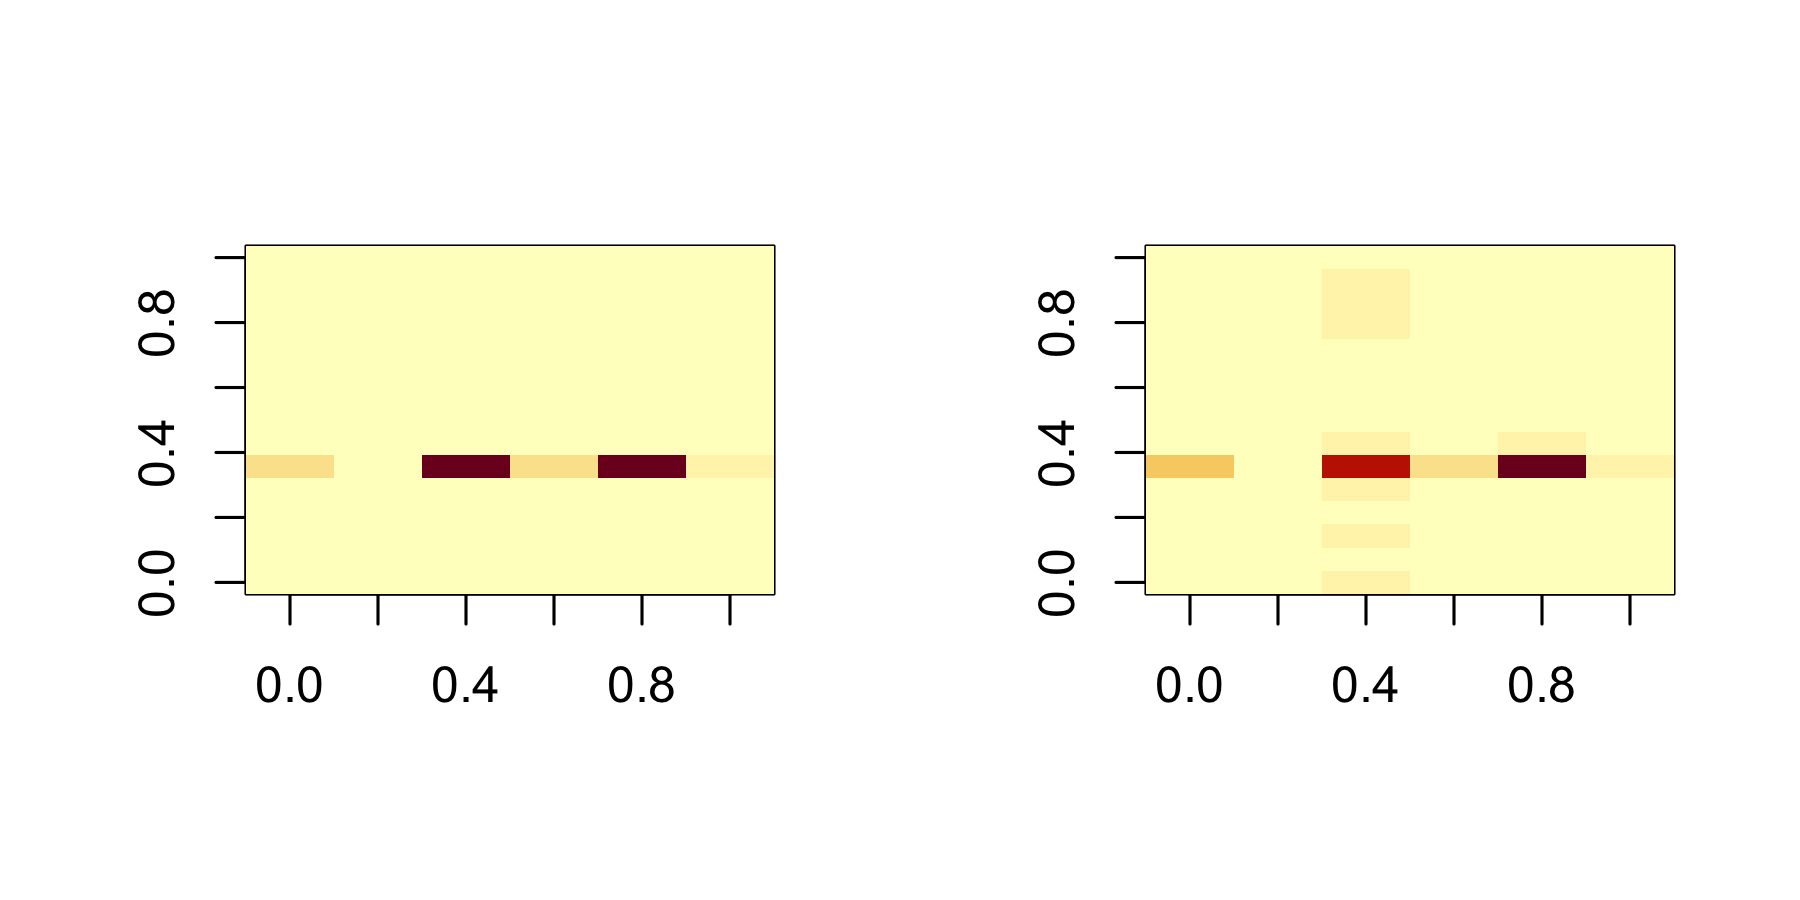
\includegraphics[width=\textwidth]{figure_roo_summary/Biliary-AdenoCA_nucleotidesubstitution1_ROOcount_matrices_all.png}\end{minipage}\begin{minipage}{.24\textwidth}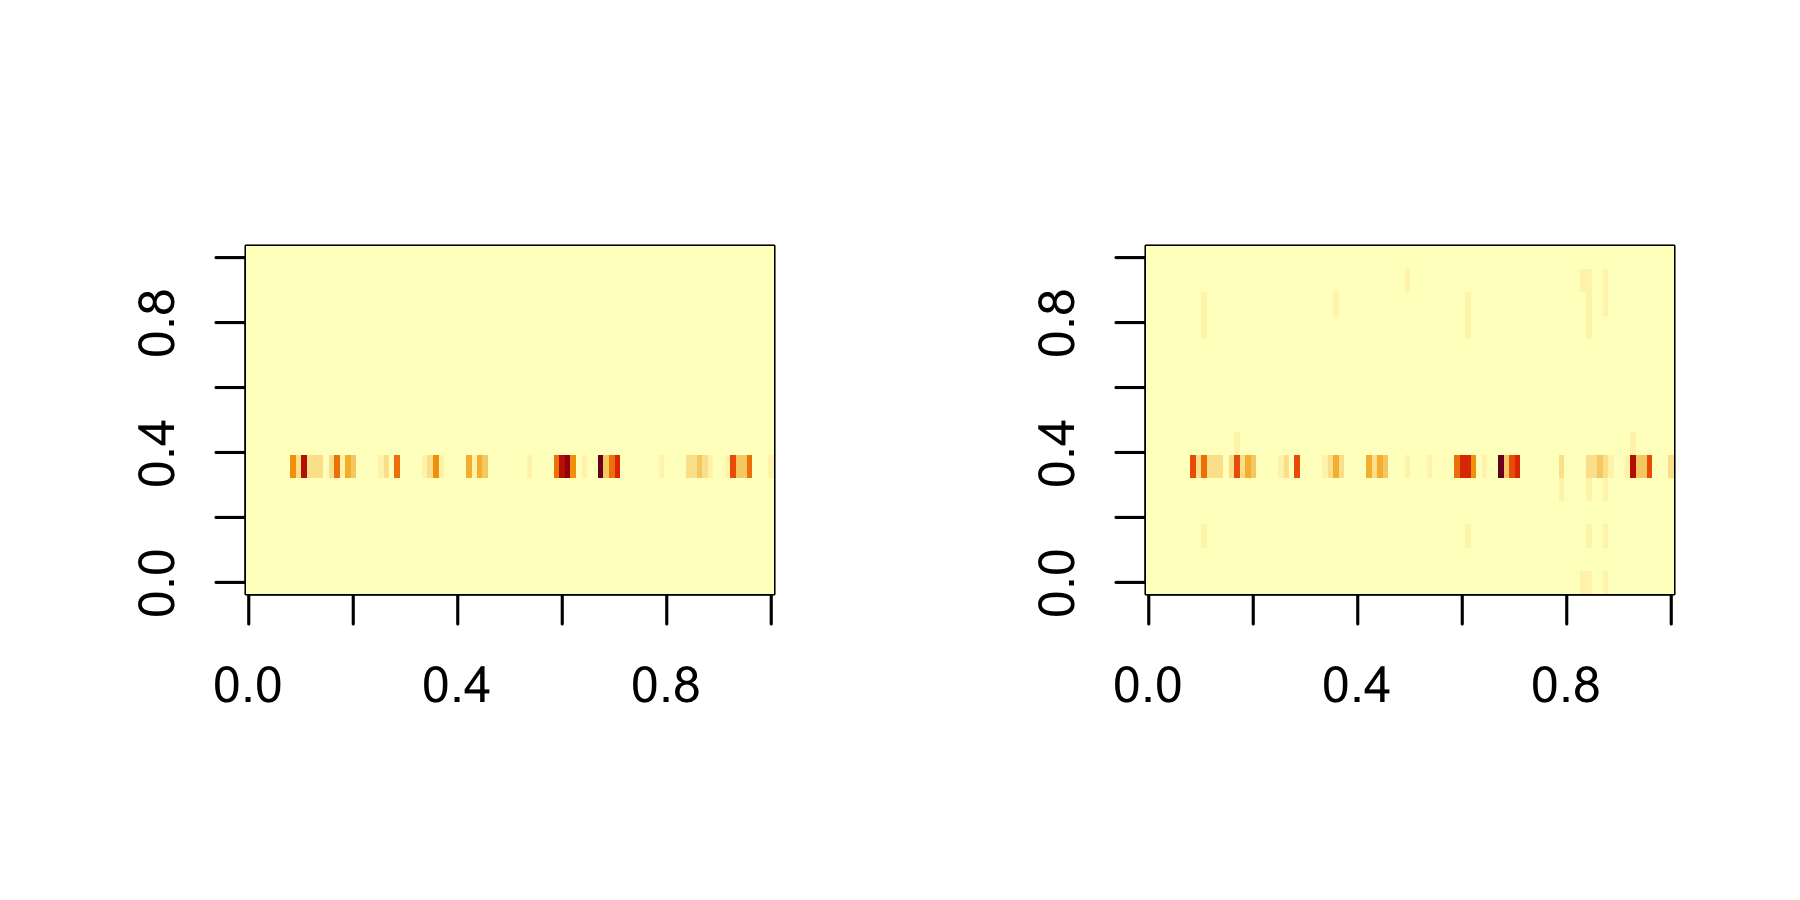
\includegraphics[width=\textwidth]{figure_roo_summary/Biliary-AdenoCA_nucleotidesubstitution3_ROOcount_matrices_all.png}\end{minipage}\begin{minipage}{.24\textwidth}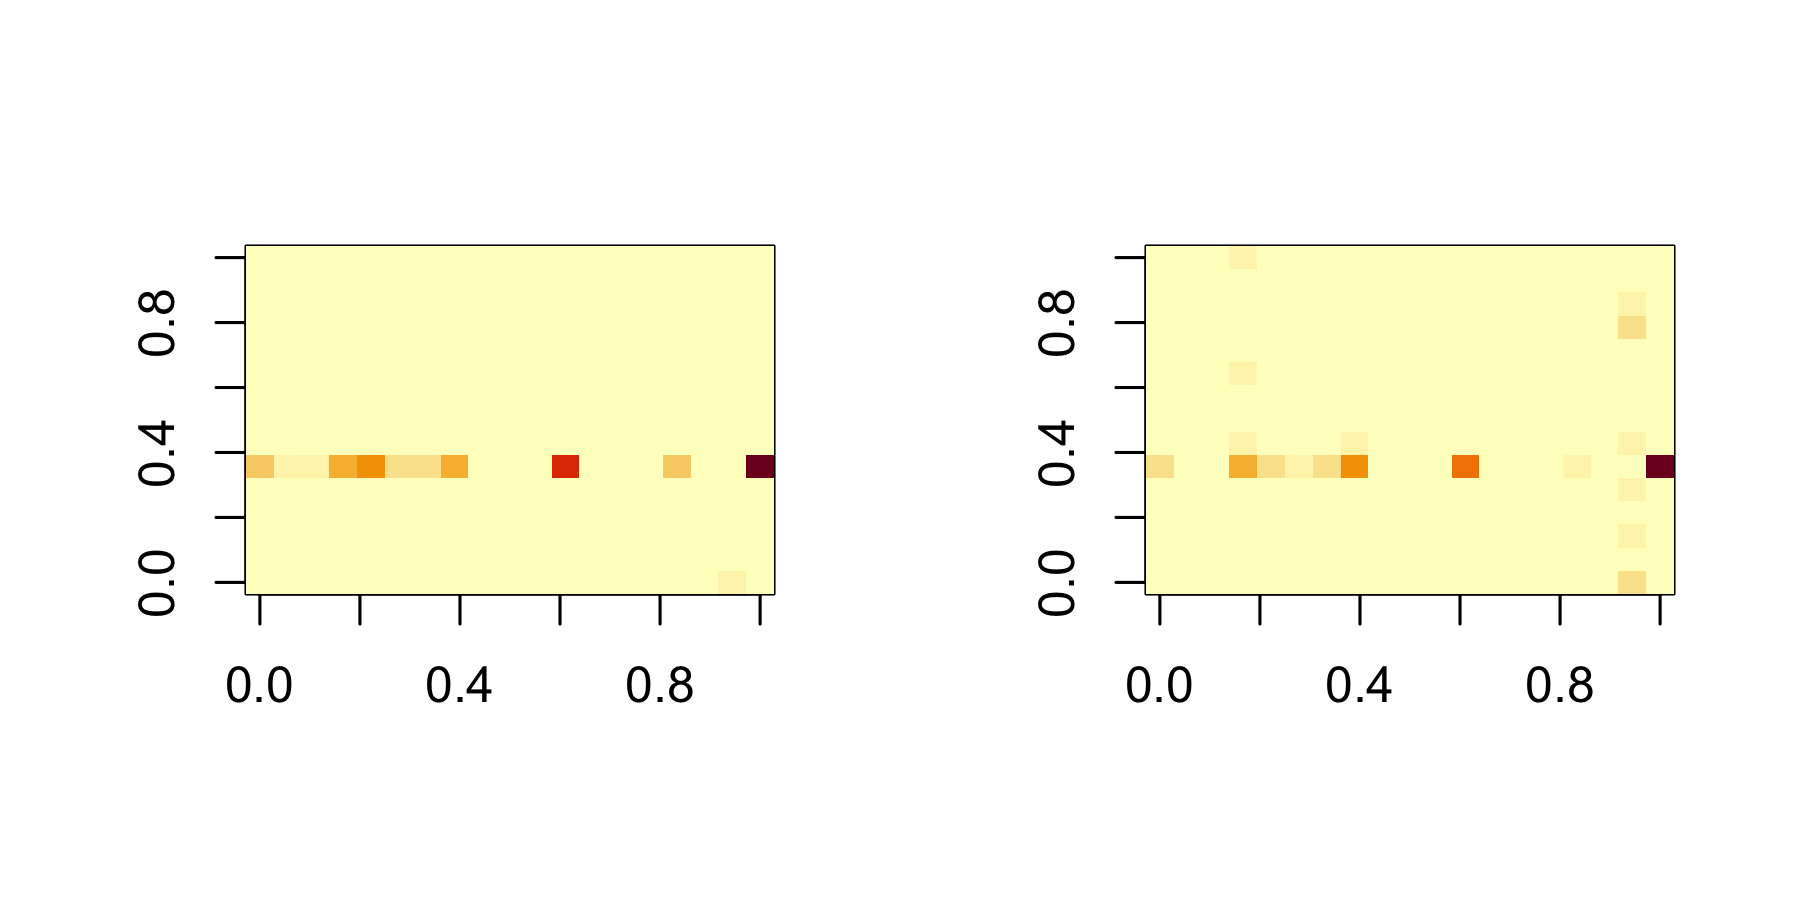
\includegraphics[width=\textwidth]{figure_roo_summary/Biliary-AdenoCA_signatures_ROOcount_matrices_active.png}\end{minipage}\begin{minipage}{.24\textwidth}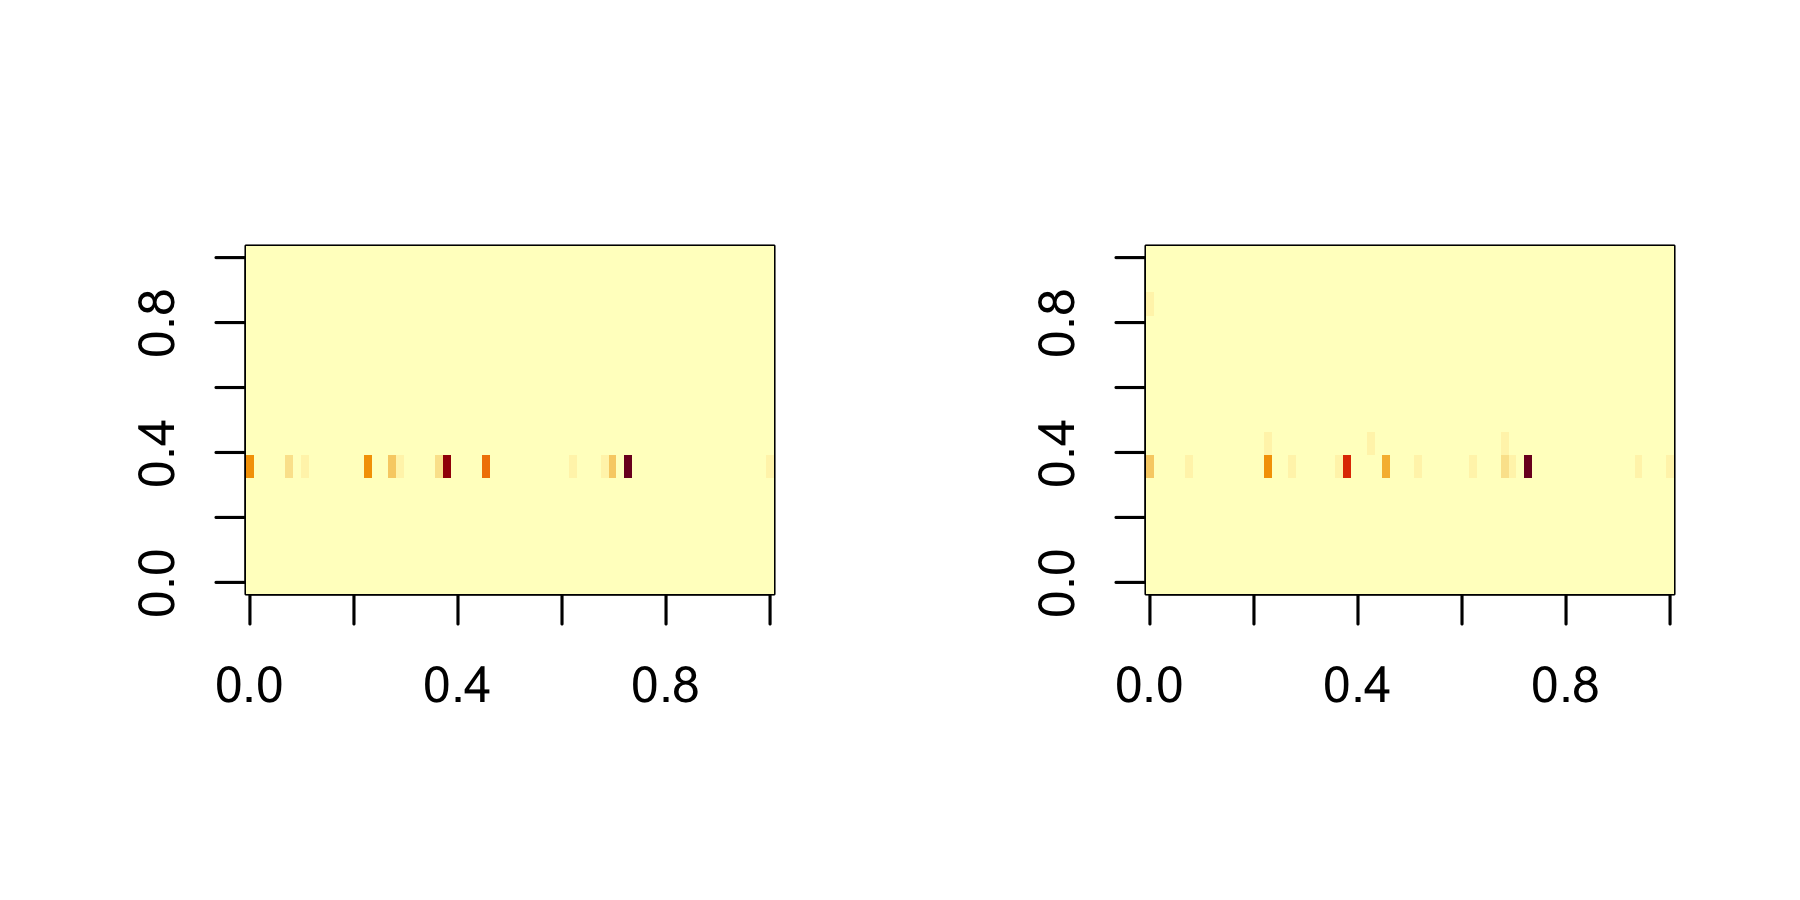
\includegraphics[width=\textwidth]{figure_roo_summary/Biliary-AdenoCA_signatures_ROOcount_matrices_all.png}\end{minipage}\caption{Biliary-AdenoCA}\end{figure}\begin{figure}\begin{minipage}{.24\textwidth}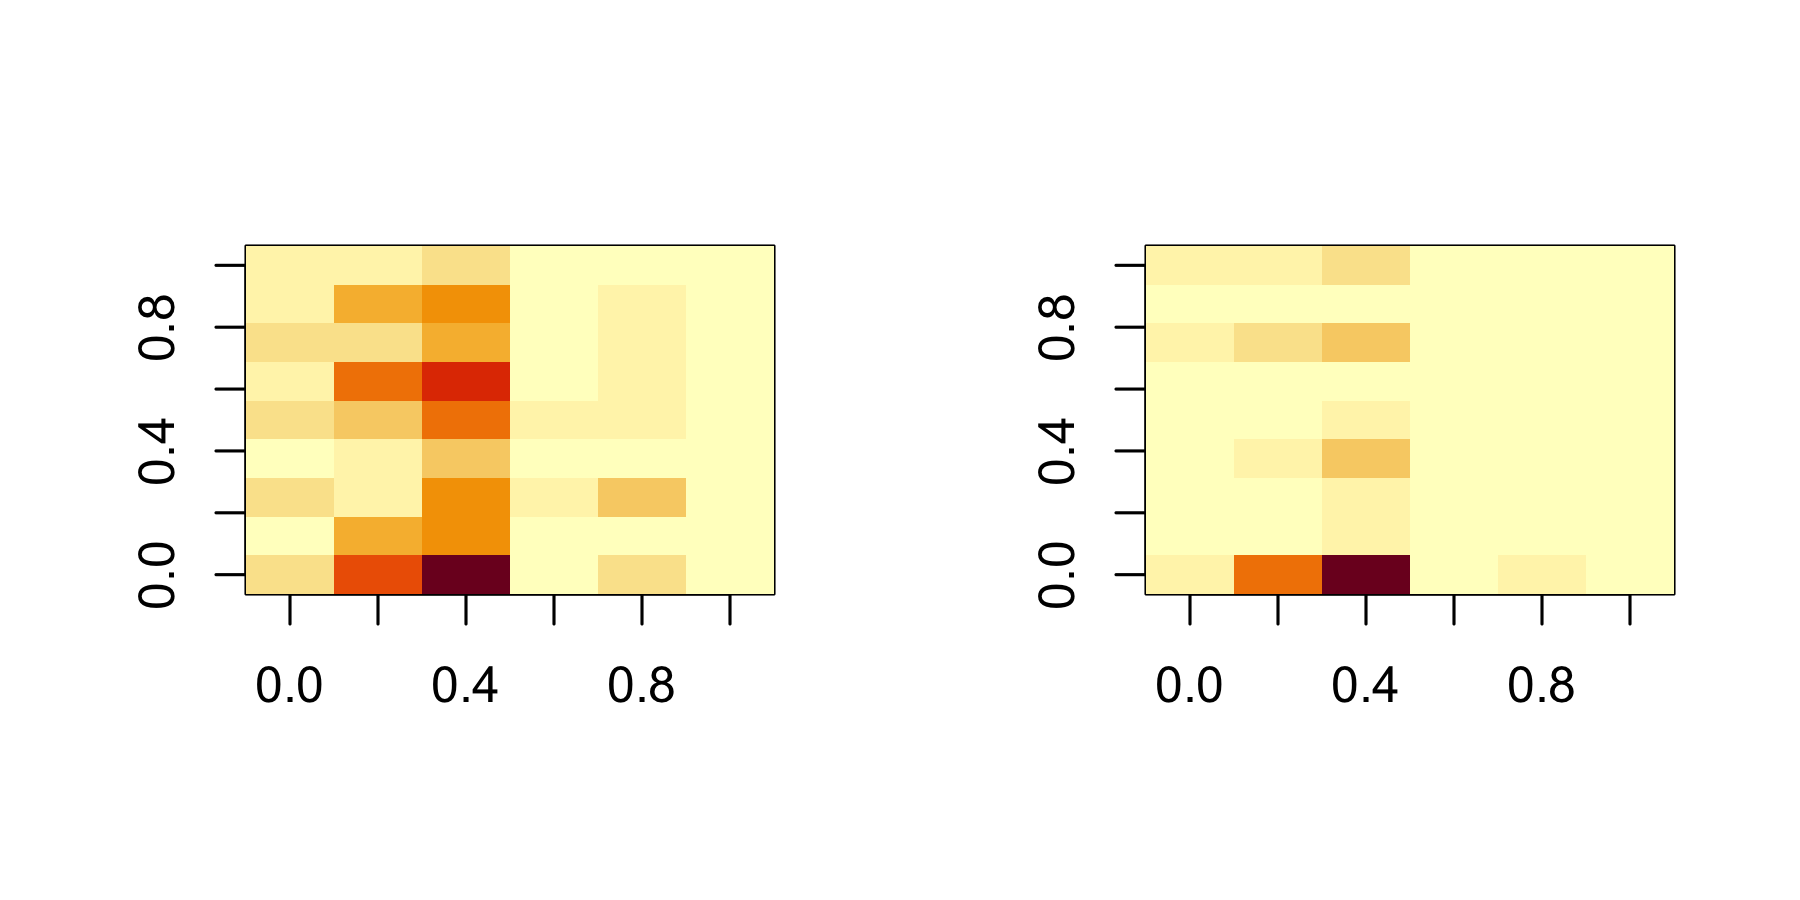
\includegraphics[width=\textwidth]{figure_roo_summary/Bladder-TCC_nucleotidesubstitution1_ROOcount_matrices_all.png}\end{minipage}\begin{minipage}{.24\textwidth}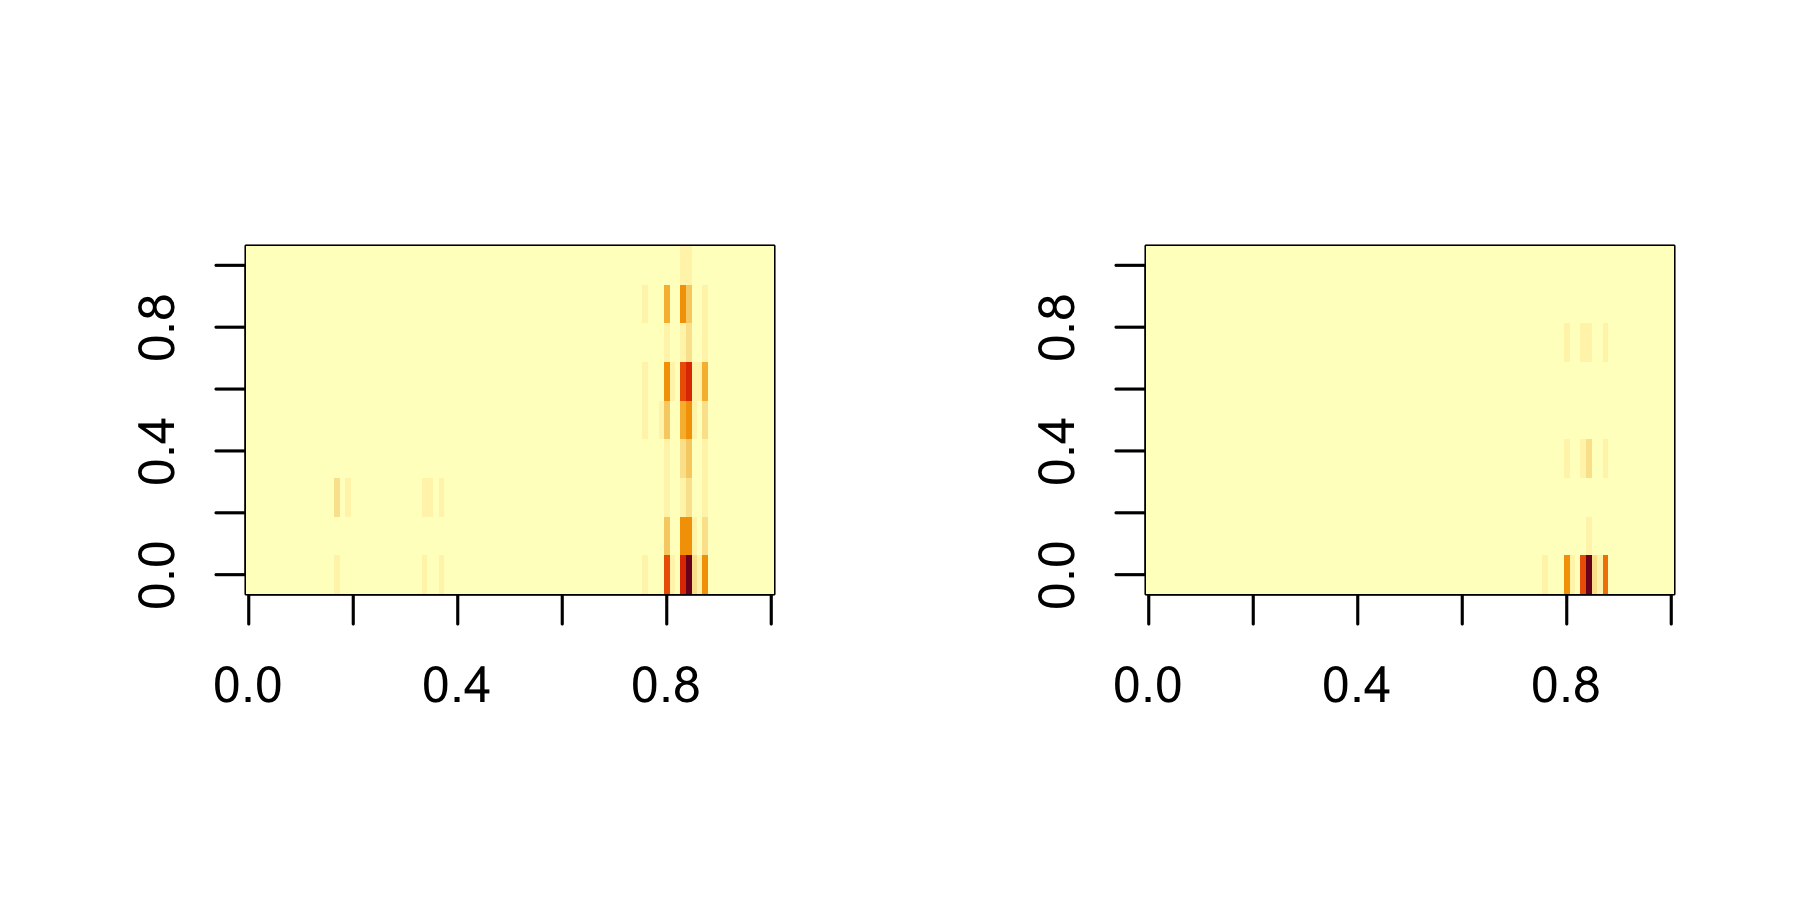
\includegraphics[width=\textwidth]{figure_roo_summary/Bladder-TCC_nucleotidesubstitution3_ROOcount_matrices_all.png}\end{minipage}\begin{minipage}{.24\textwidth}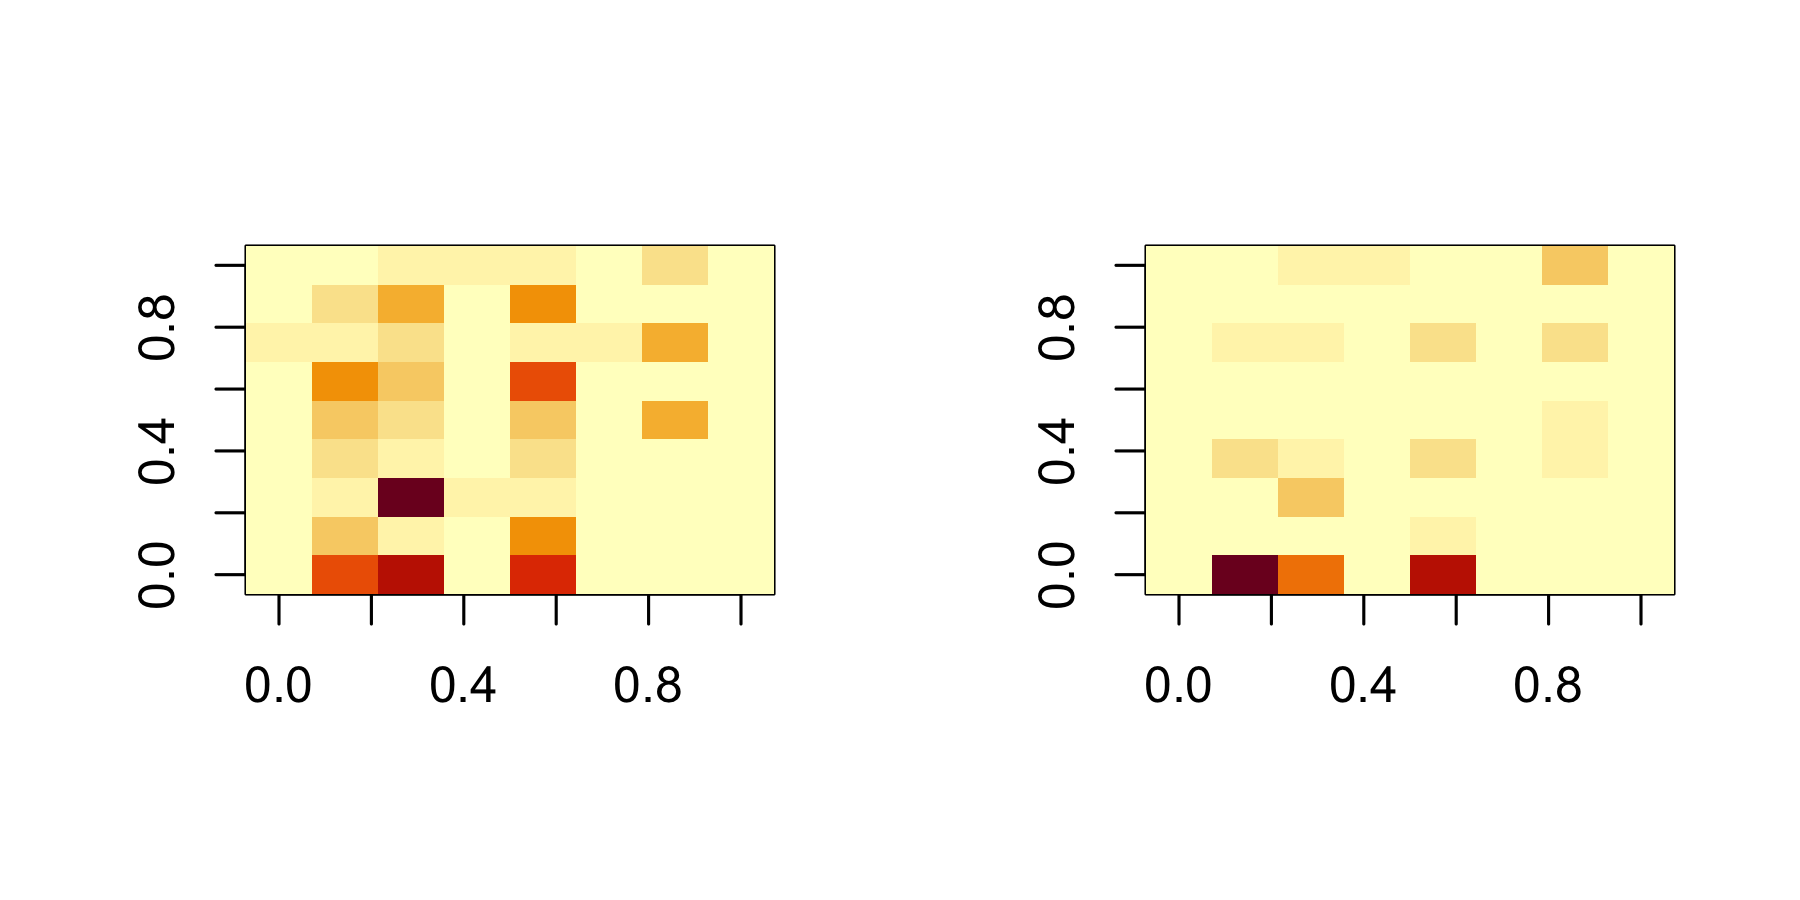
\includegraphics[width=\textwidth]{figure_roo_summary/Bladder-TCC_signatures_ROOcount_matrices_active.png}\end{minipage}\begin{minipage}{.24\textwidth}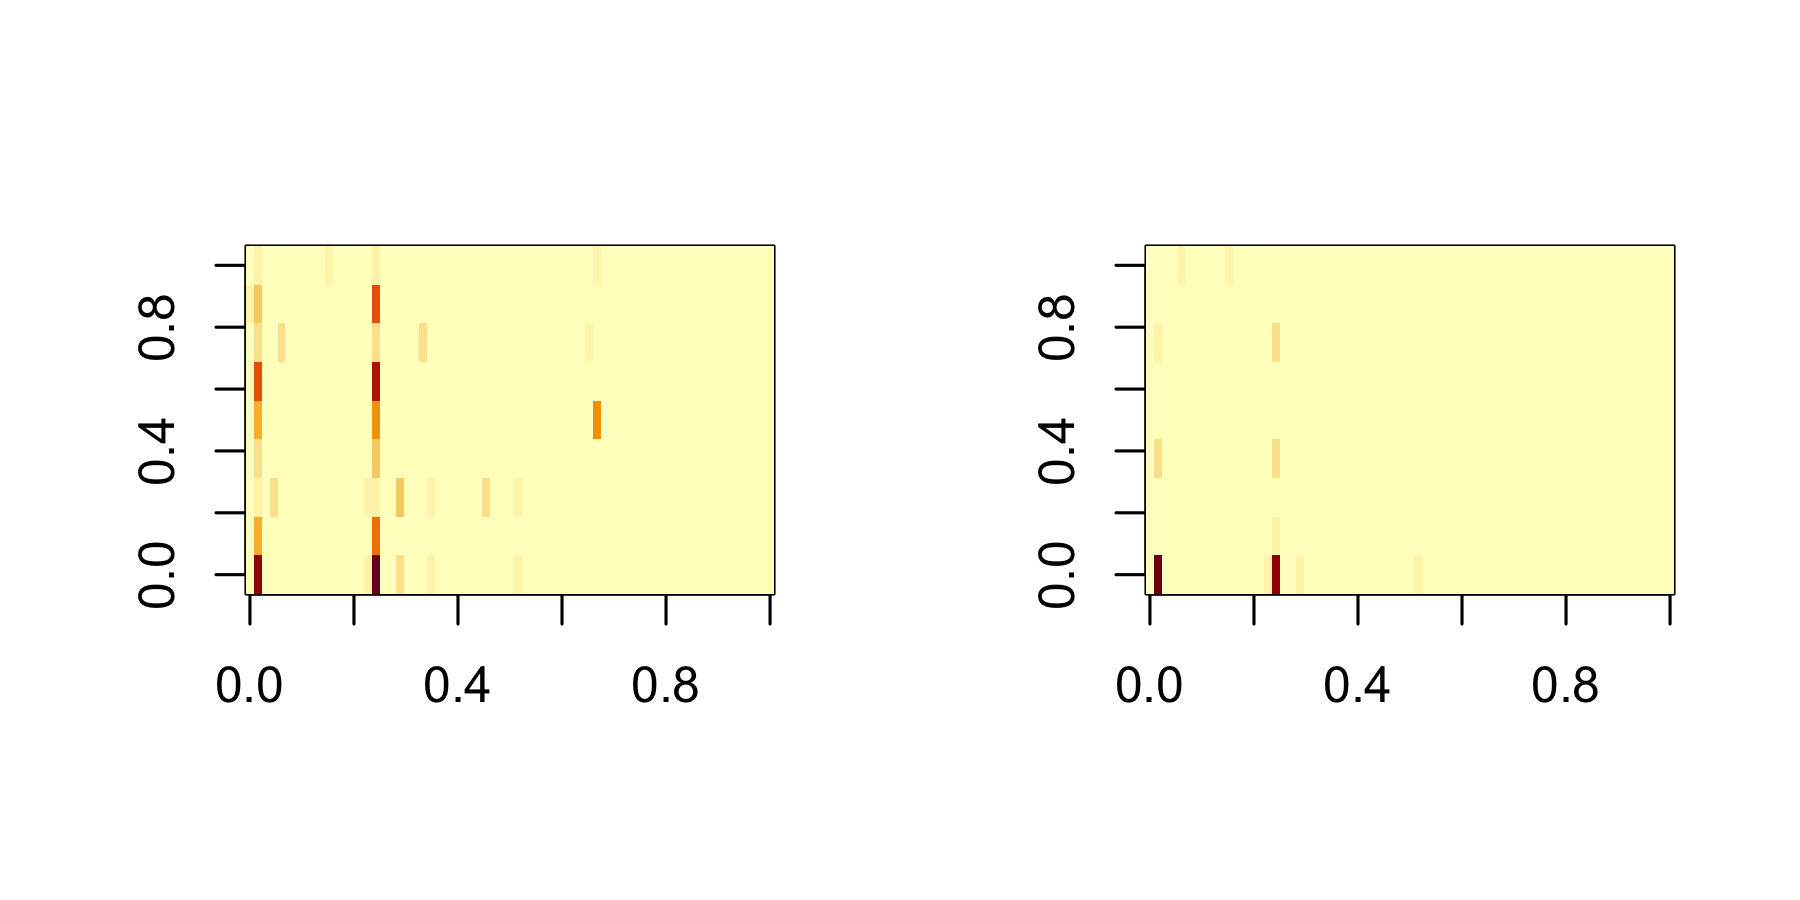
\includegraphics[width=\textwidth]{figure_roo_summary/Bladder-TCC_signatures_ROOcount_matrices_all.png}\end{minipage}\caption{Bladder-TCC}\end{figure}\begin{figure}\begin{minipage}{.24\textwidth}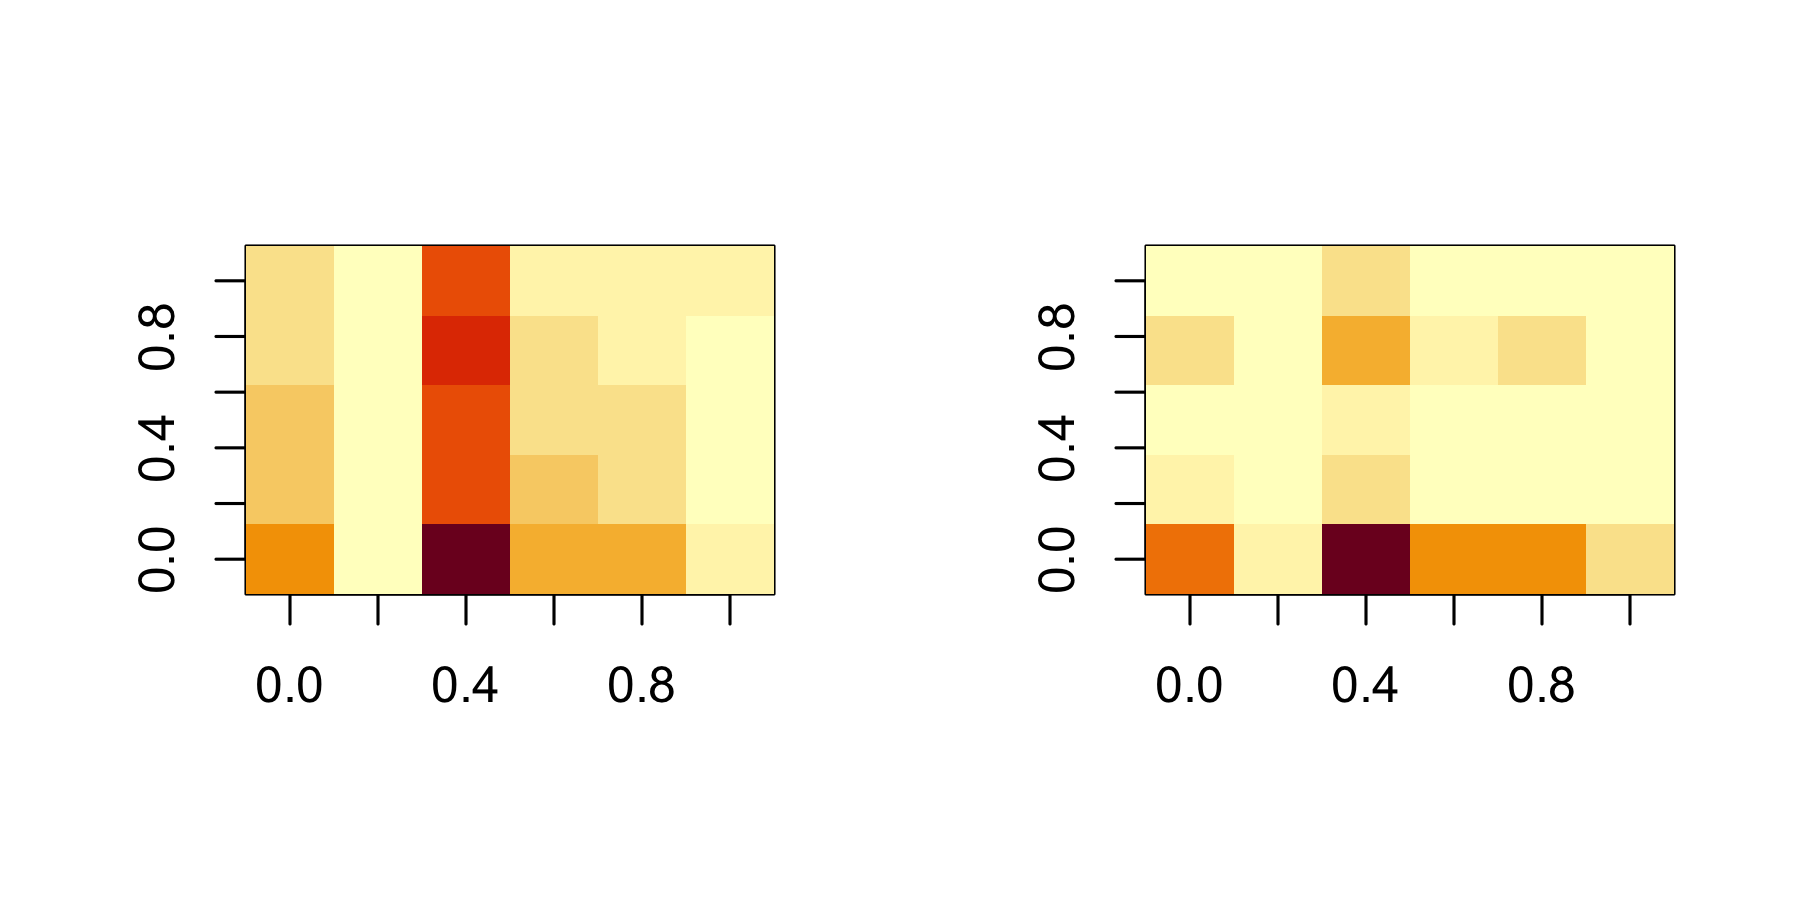
\includegraphics[width=\textwidth]{figure_roo_summary/Bone-Benign_nucleotidesubstitution1_ROOcount_matrices_all.png}\end{minipage}\begin{minipage}{.24\textwidth}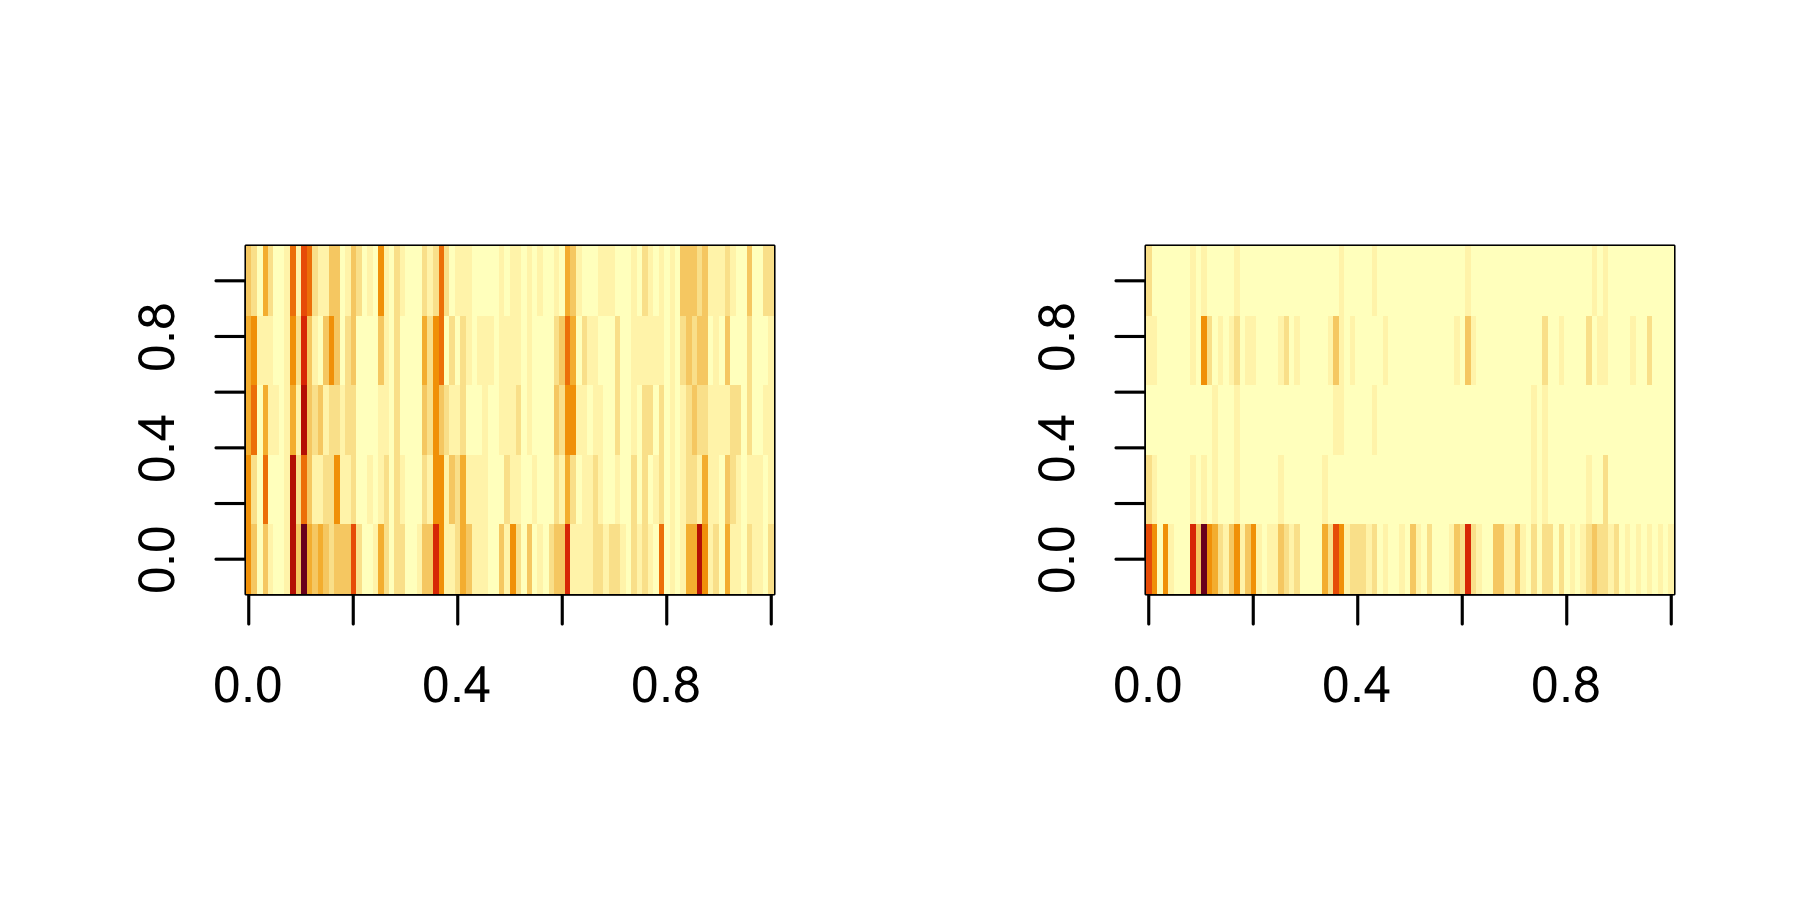
\includegraphics[width=\textwidth]{figure_roo_summary/Bone-Benign_nucleotidesubstitution3_ROOcount_matrices_all.png}\end{minipage}\begin{minipage}{.24\textwidth}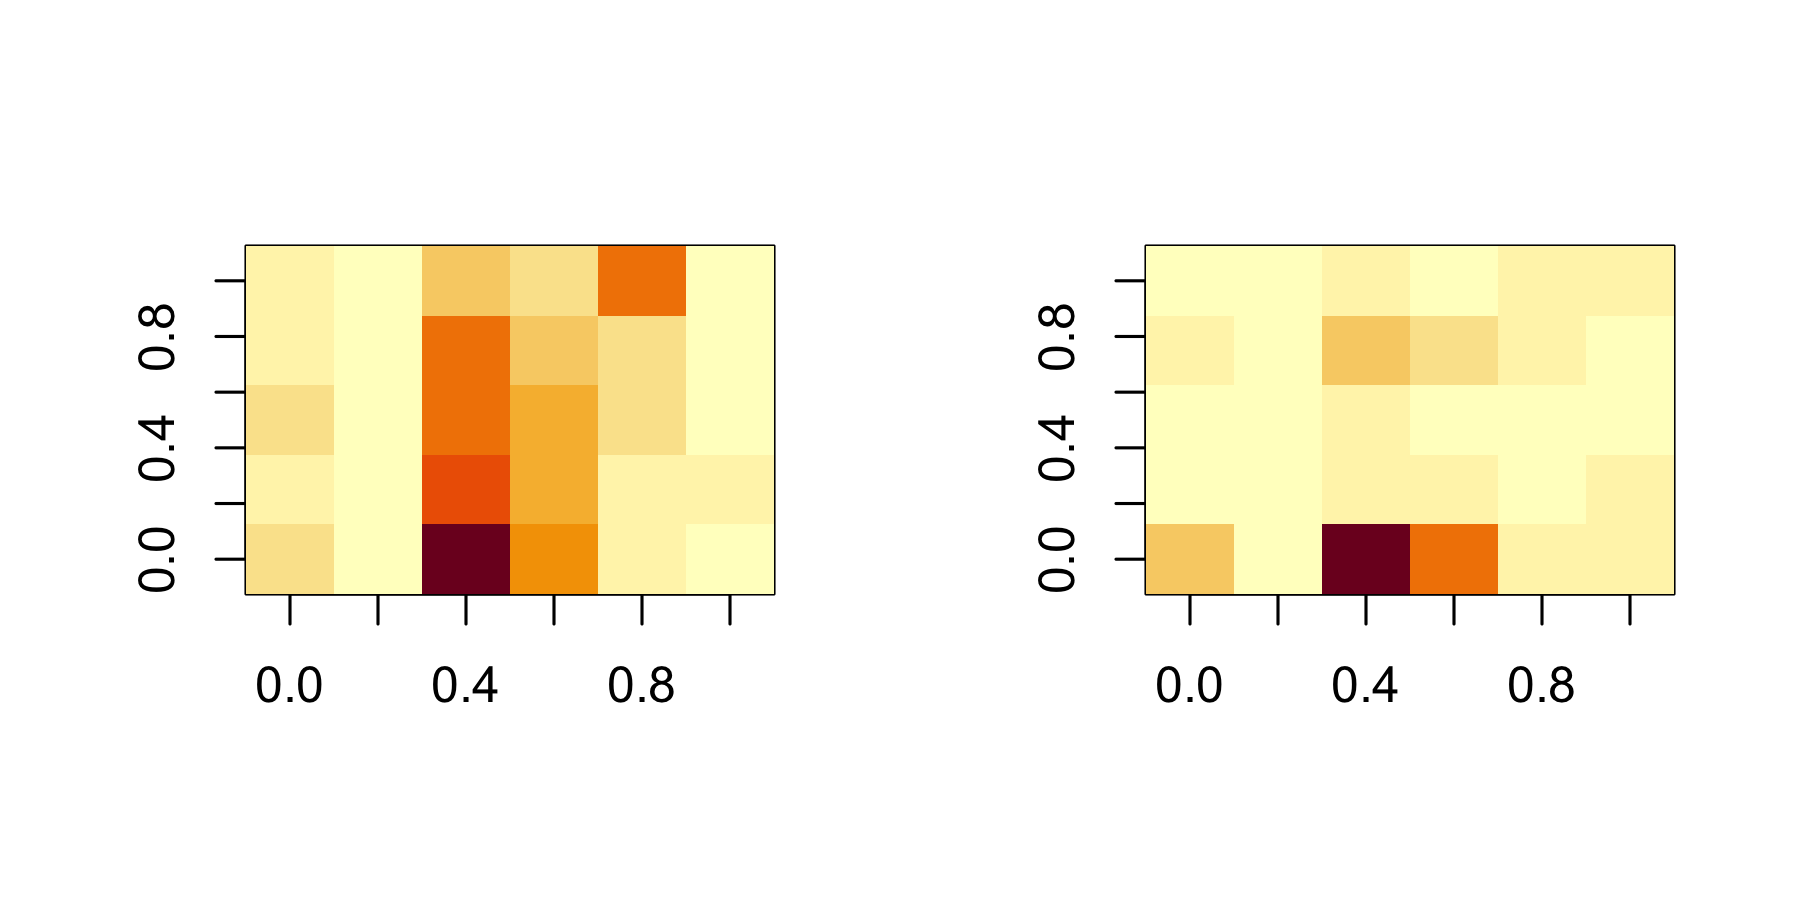
\includegraphics[width=\textwidth]{figure_roo_summary/Bone-Benign_signatures_ROOcount_matrices_active.png}\end{minipage}\begin{minipage}{.24\textwidth}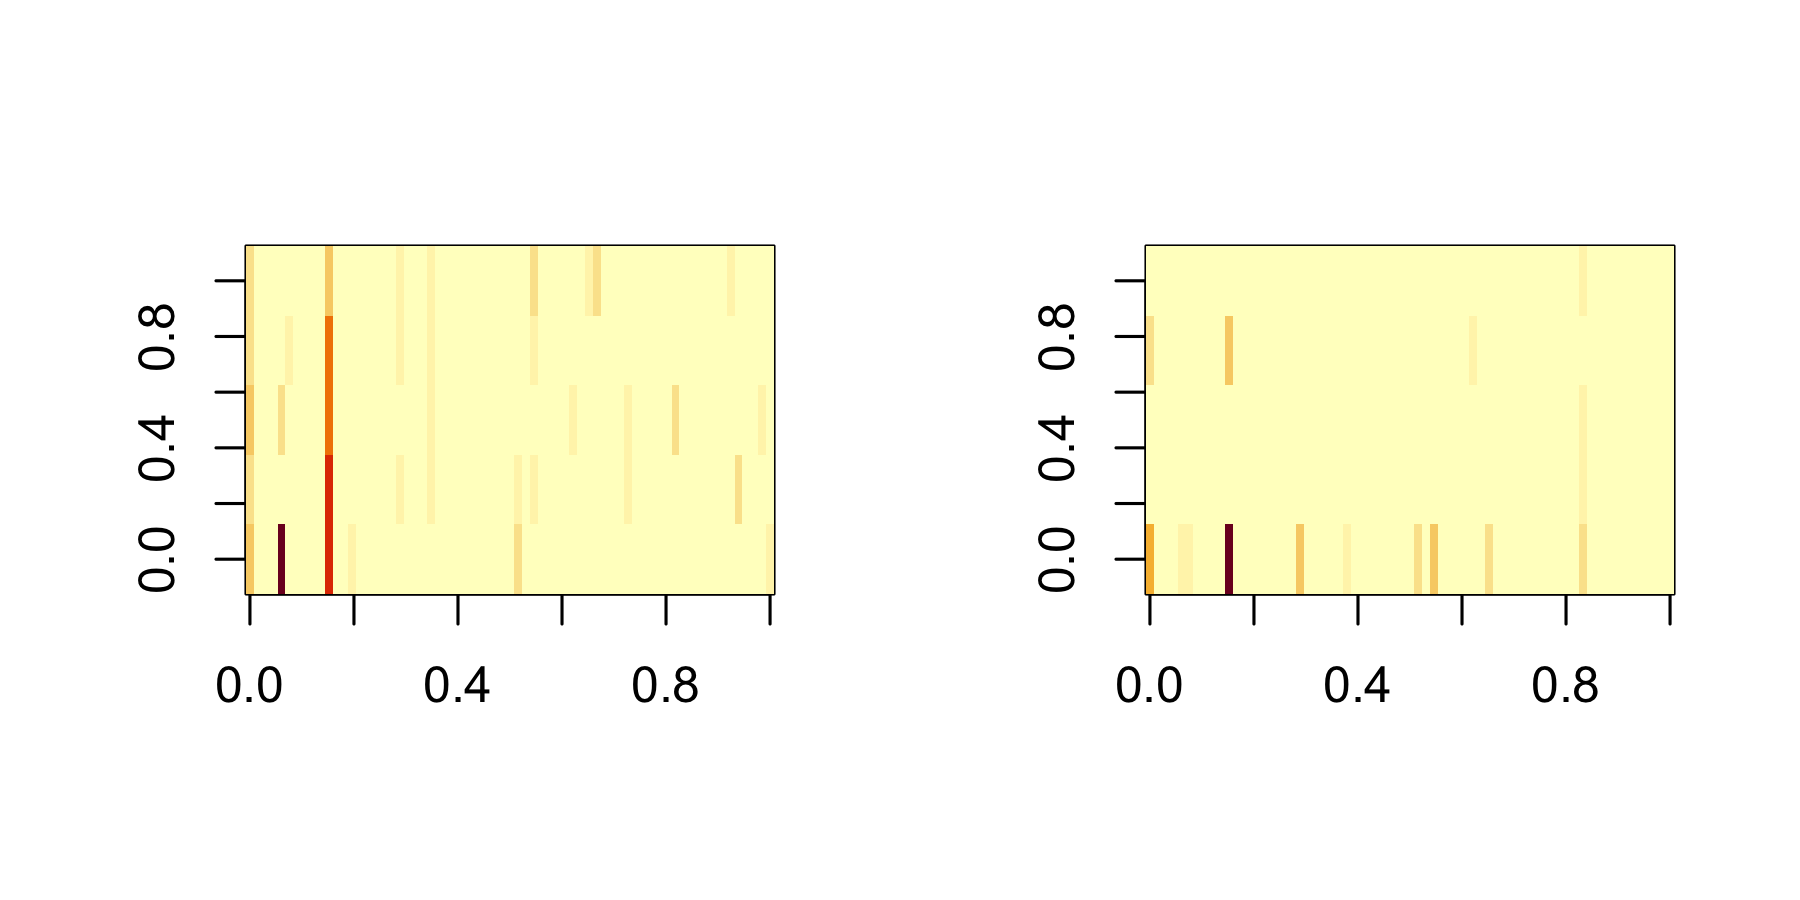
\includegraphics[width=\textwidth]{figure_roo_summary/Bone-Benign_signatures_ROOcount_matrices_all.png}\end{minipage}\caption{Bone-Benign}\end{figure}\begin{figure}\begin{minipage}{.24\textwidth}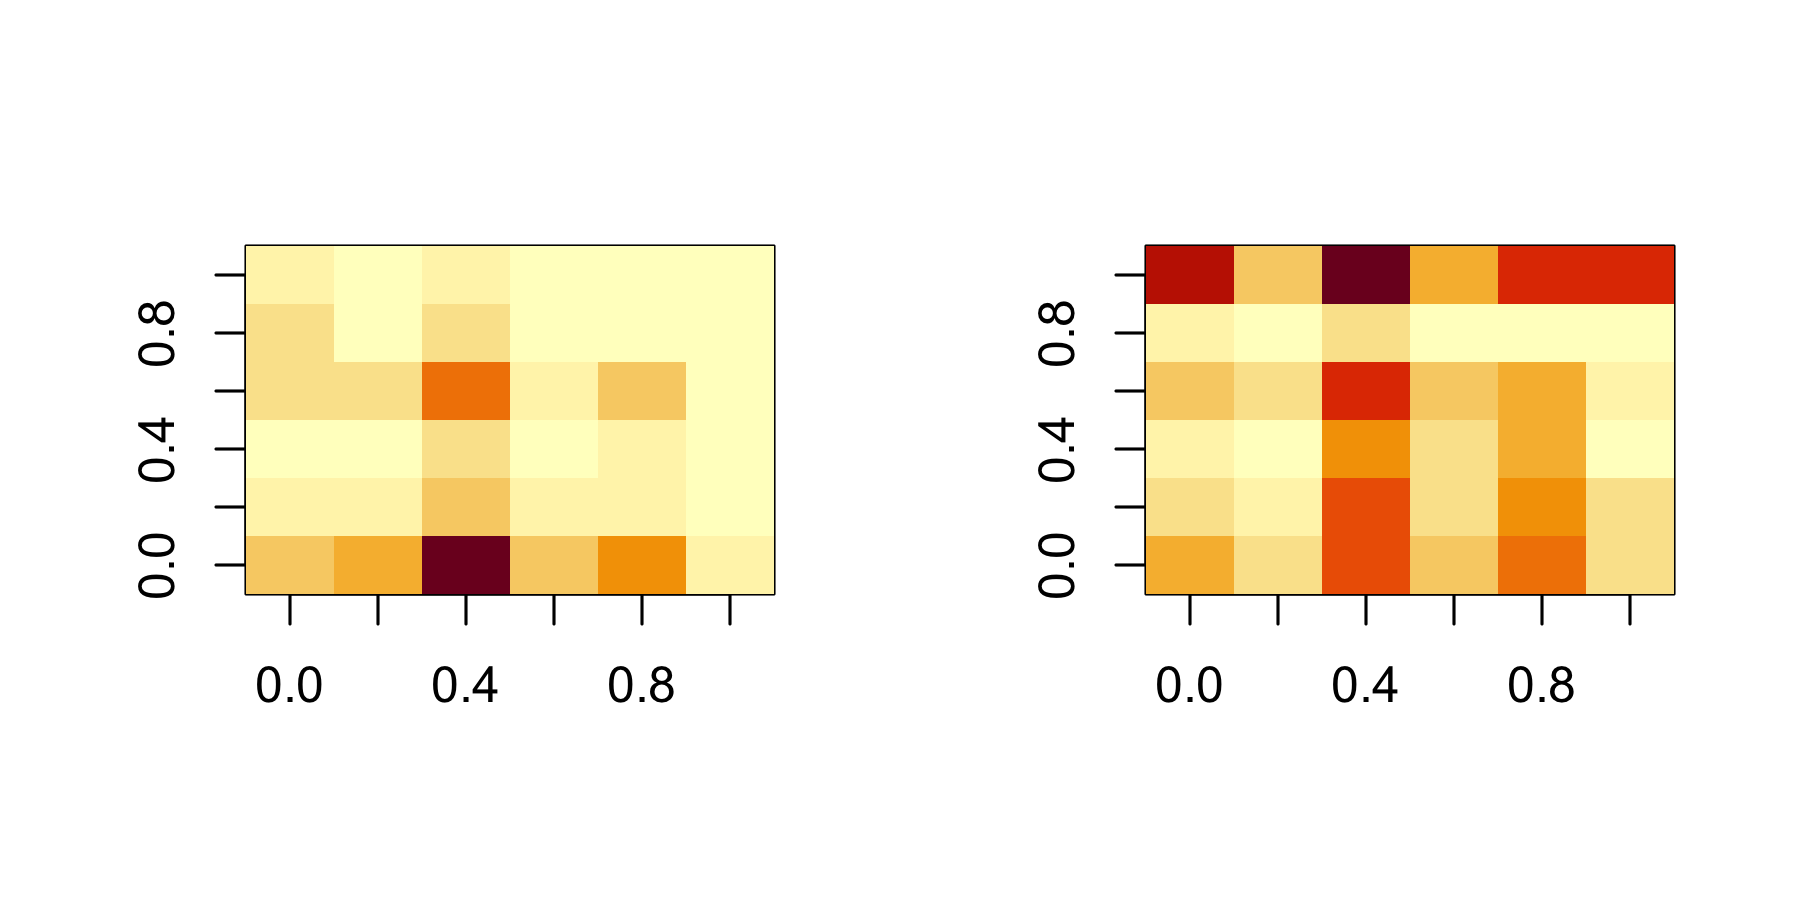
\includegraphics[width=\textwidth]{figure_roo_summary/Bone-Epith_nucleotidesubstitution1_ROOcount_matrices_all.png}\end{minipage}\begin{minipage}{.24\textwidth}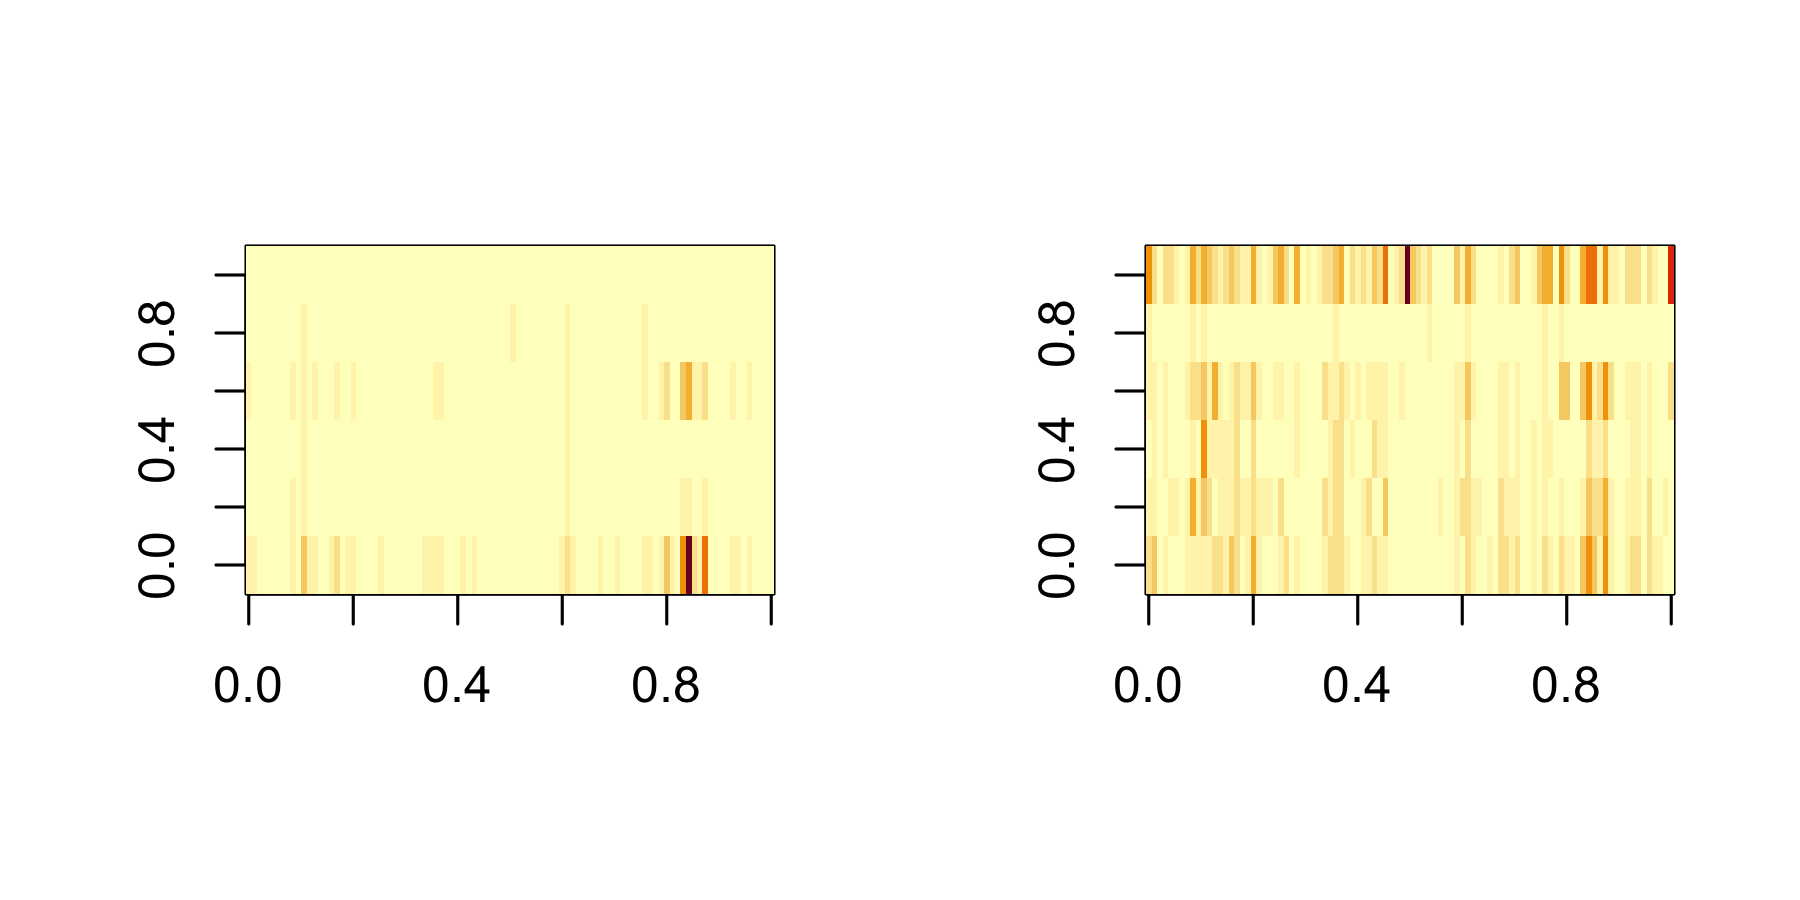
\includegraphics[width=\textwidth]{figure_roo_summary/Bone-Epith_nucleotidesubstitution3_ROOcount_matrices_all.png}\end{minipage}\begin{minipage}{.24\textwidth}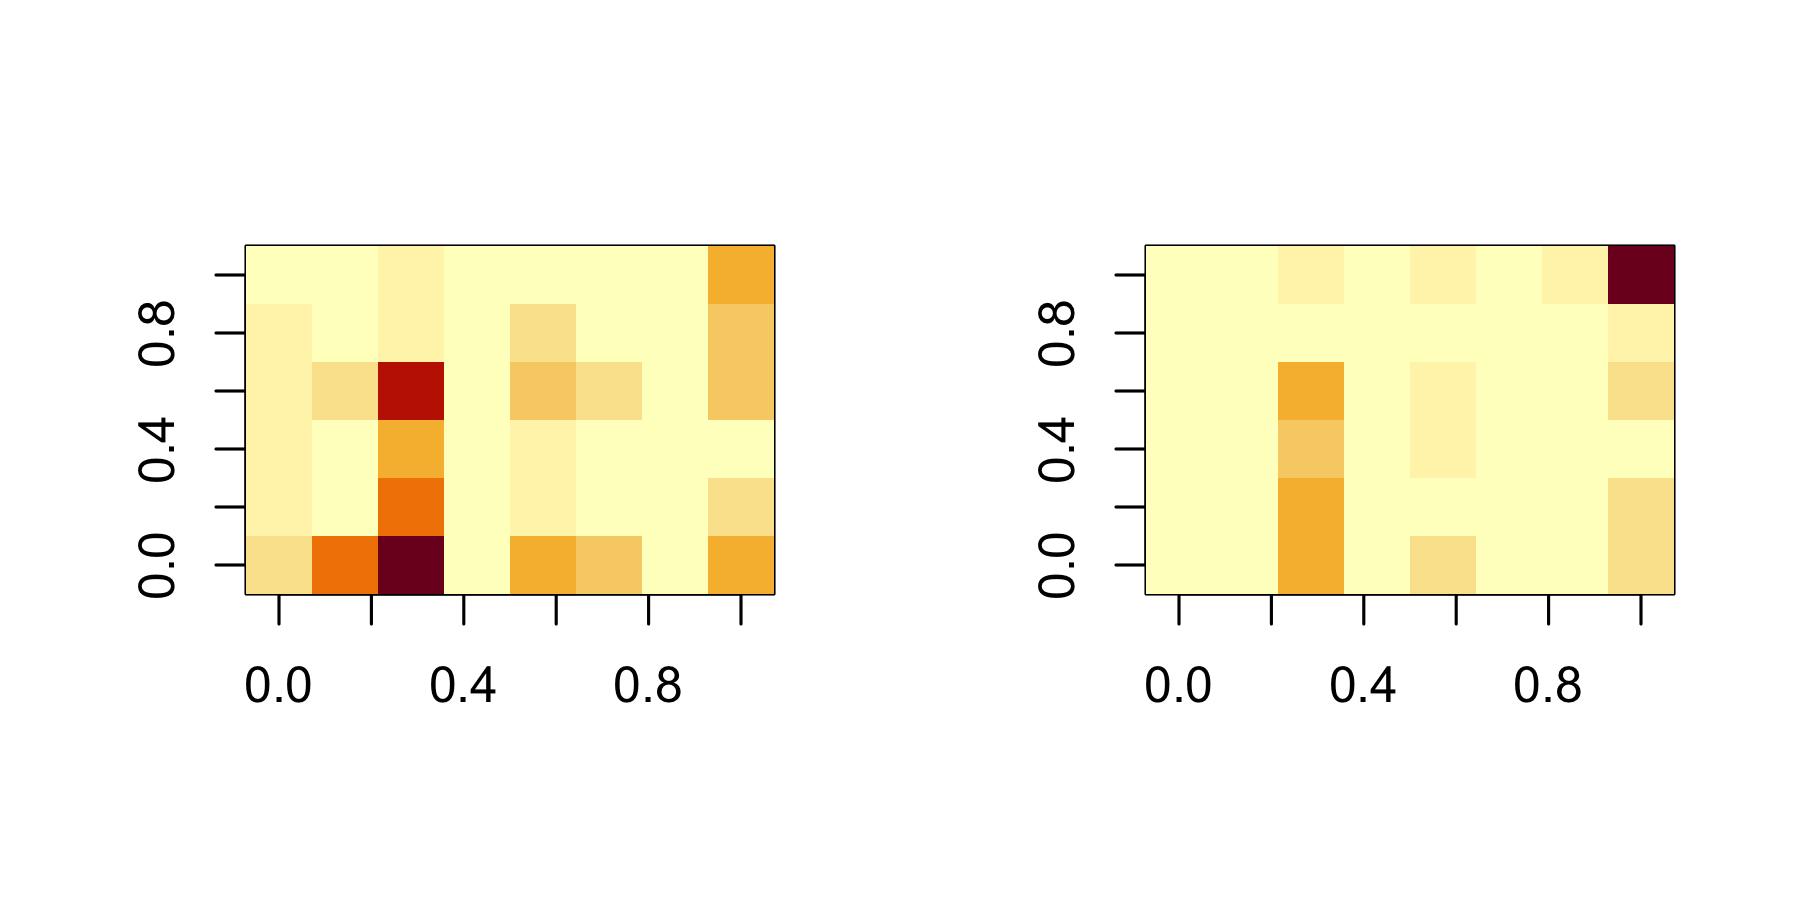
\includegraphics[width=\textwidth]{figure_roo_summary/Bone-Epith_signatures_ROOcount_matrices_active.png}\end{minipage}\begin{minipage}{.24\textwidth}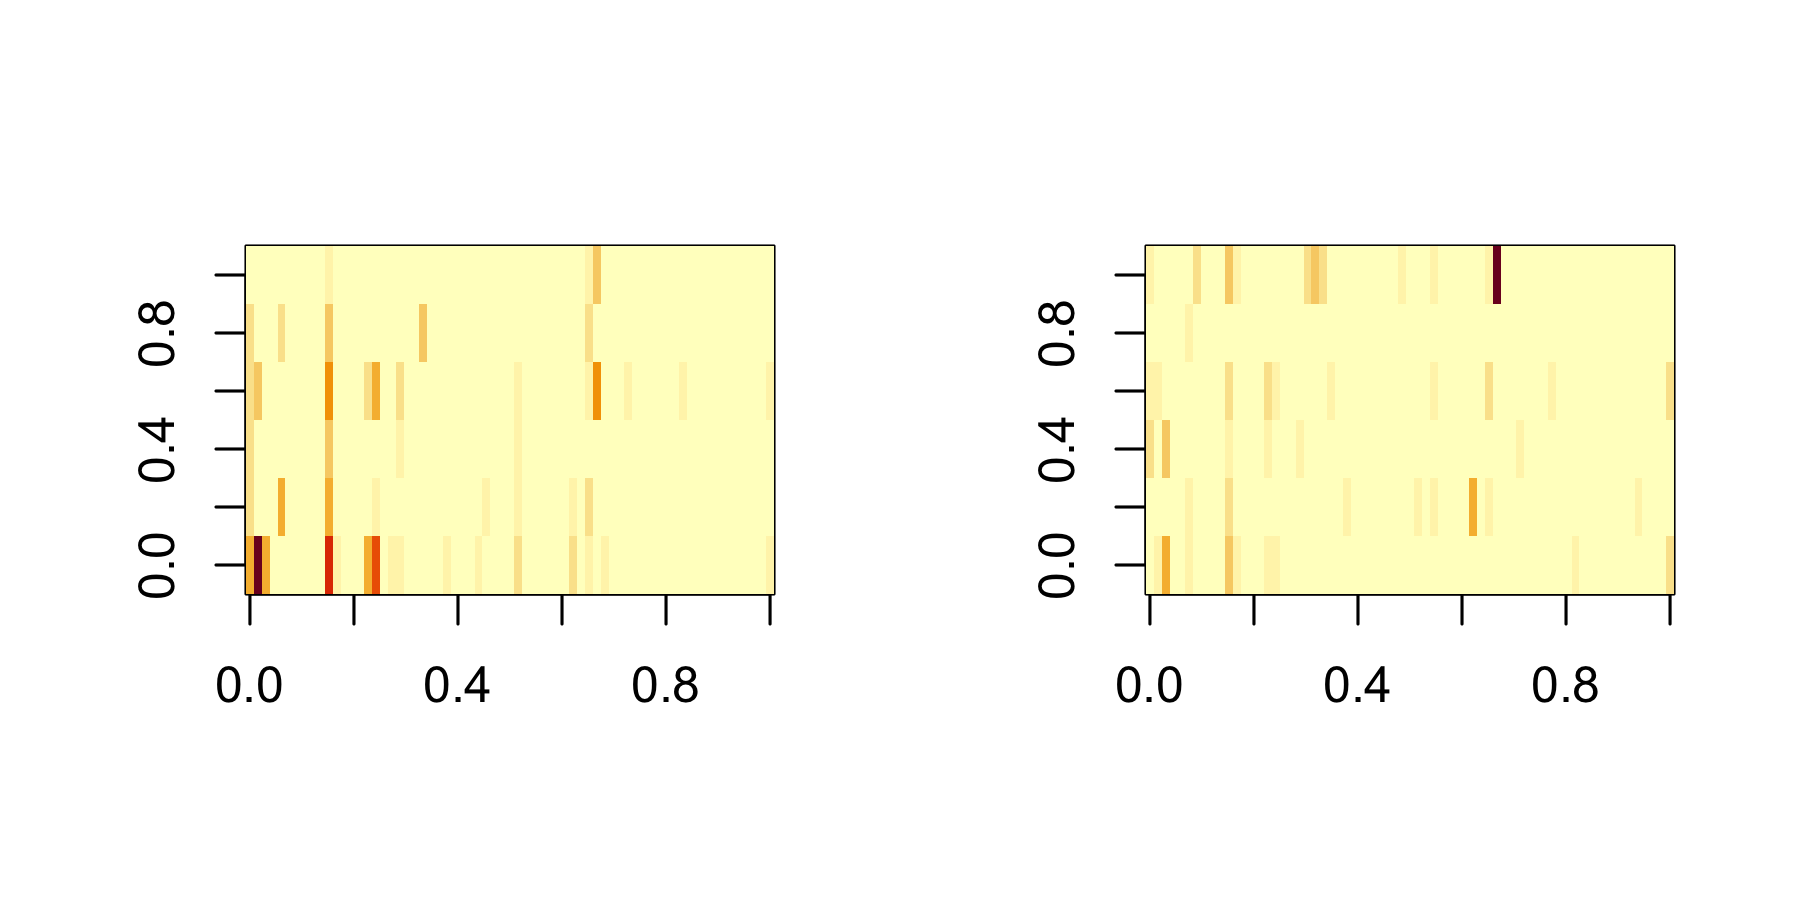
\includegraphics[width=\textwidth]{figure_roo_summary/Bone-Epith_signatures_ROOcount_matrices_all.png}\end{minipage}\caption{Bone-Epith}\end{figure}\begin{figure}\begin{minipage}{.24\textwidth}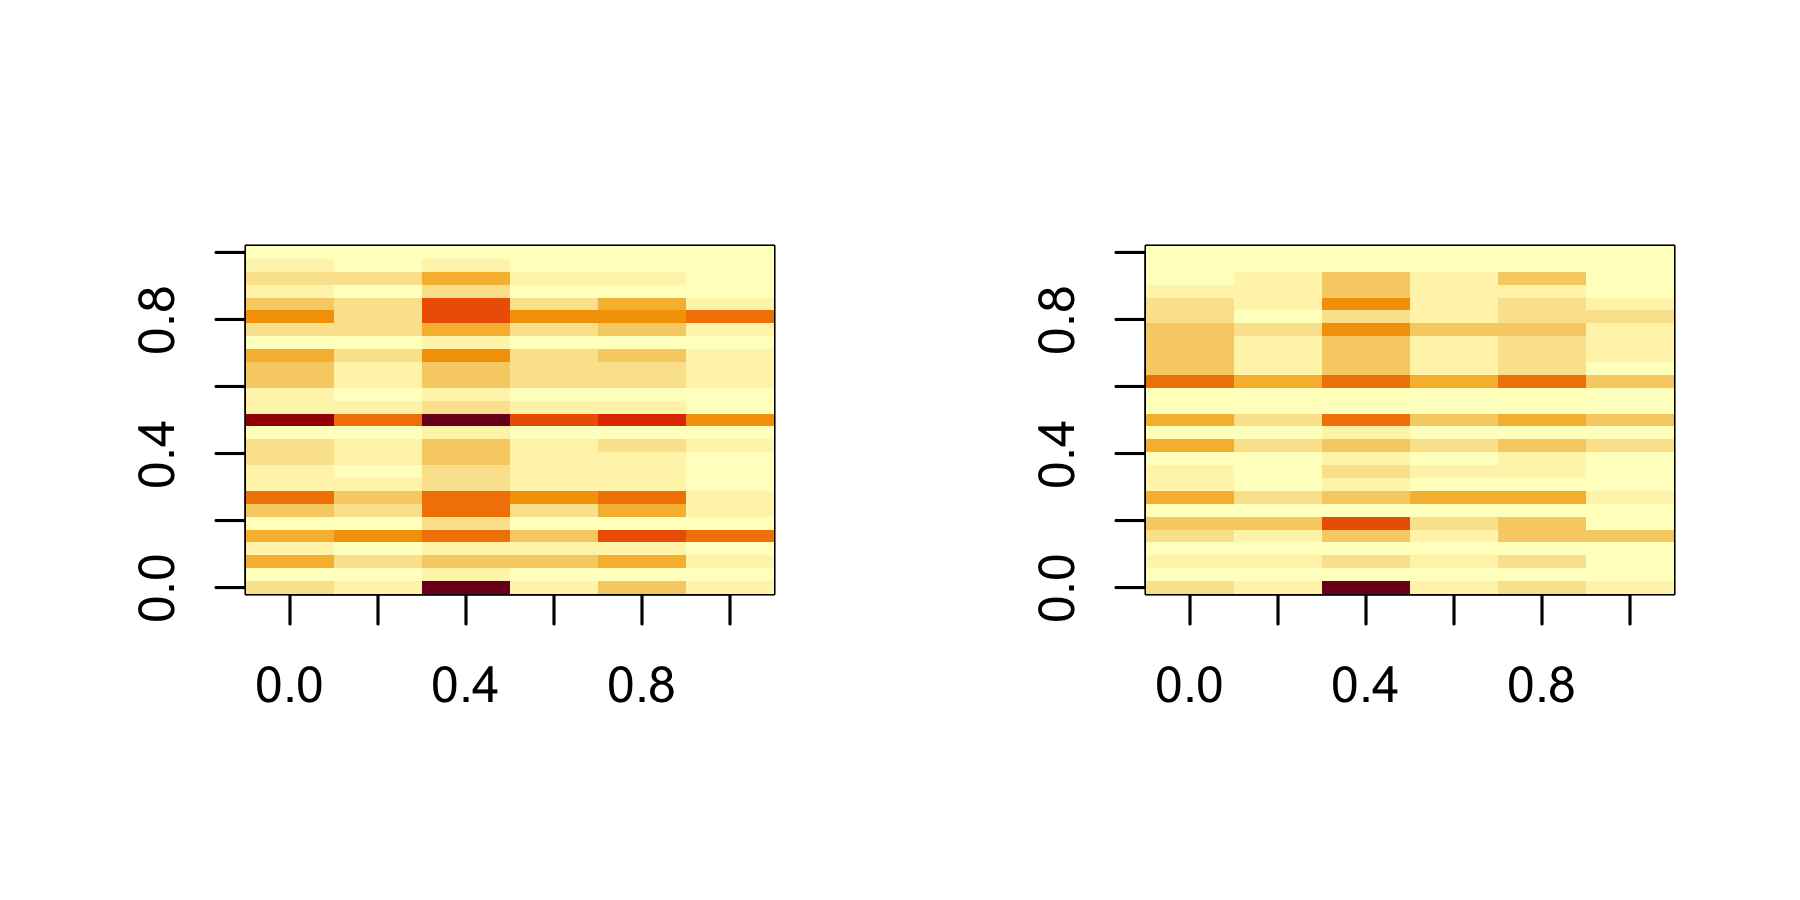
\includegraphics[width=\textwidth]{figure_roo_summary/Bone-Osteosarc_nucleotidesubstitution1_ROOcount_matrices_all.png}\end{minipage}\begin{minipage}{.24\textwidth}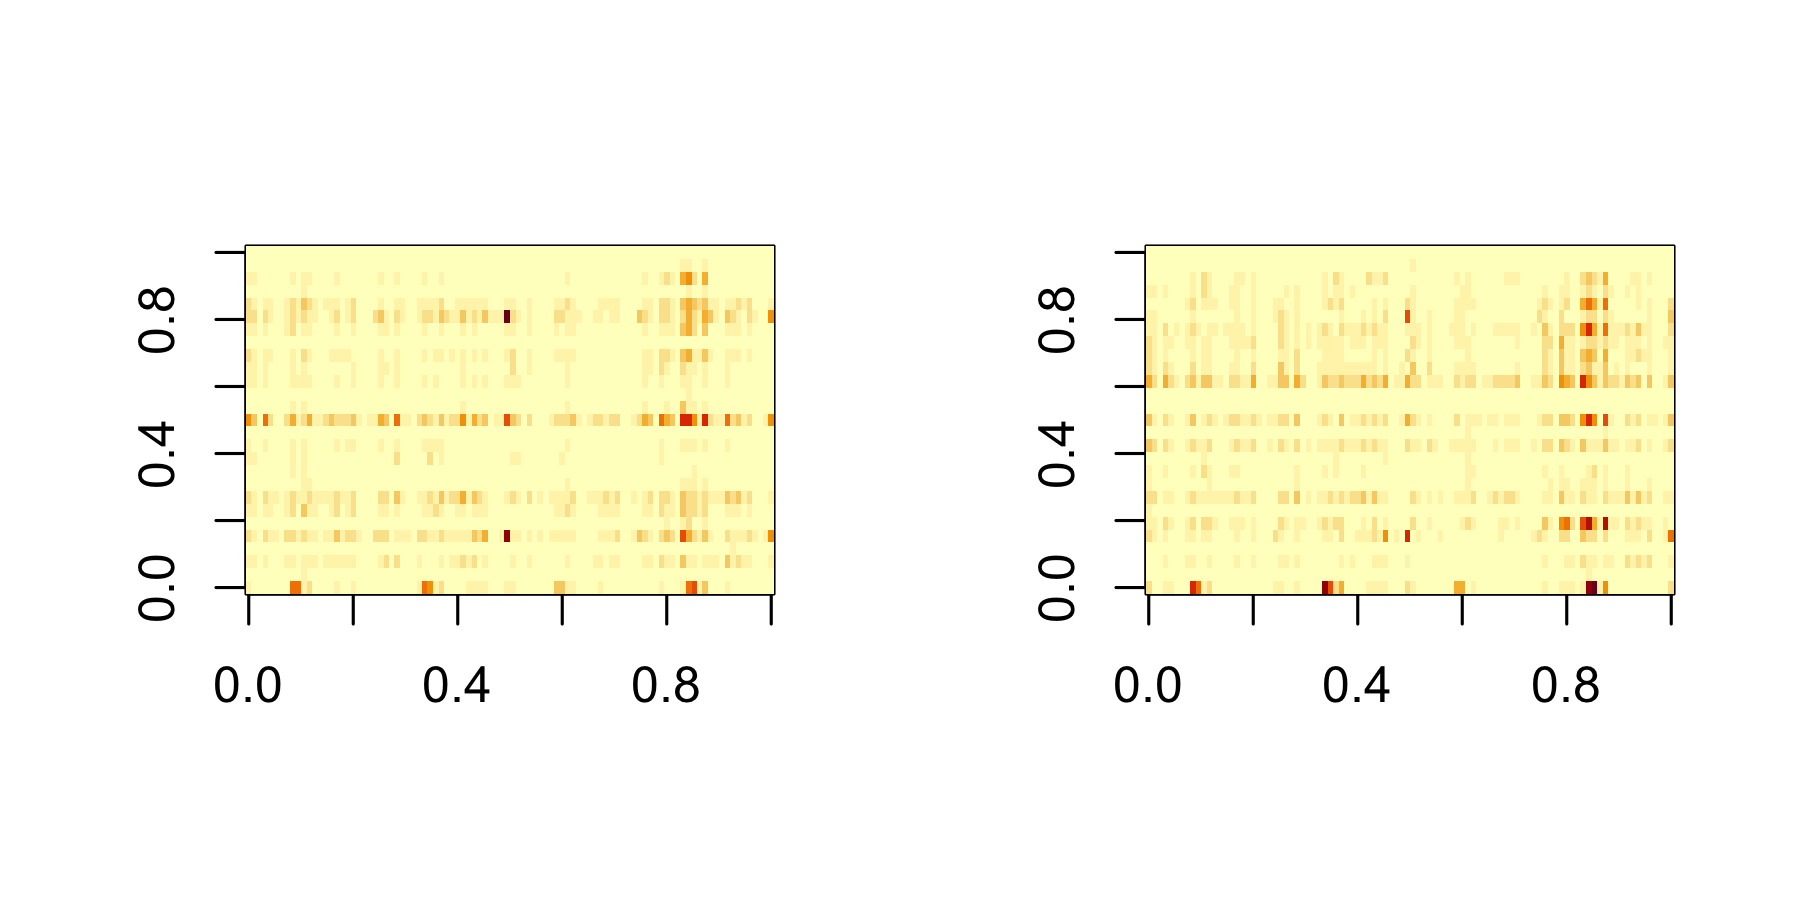
\includegraphics[width=\textwidth]{figure_roo_summary/Bone-Osteosarc_nucleotidesubstitution3_ROOcount_matrices_all.png}\end{minipage}\begin{minipage}{.24\textwidth}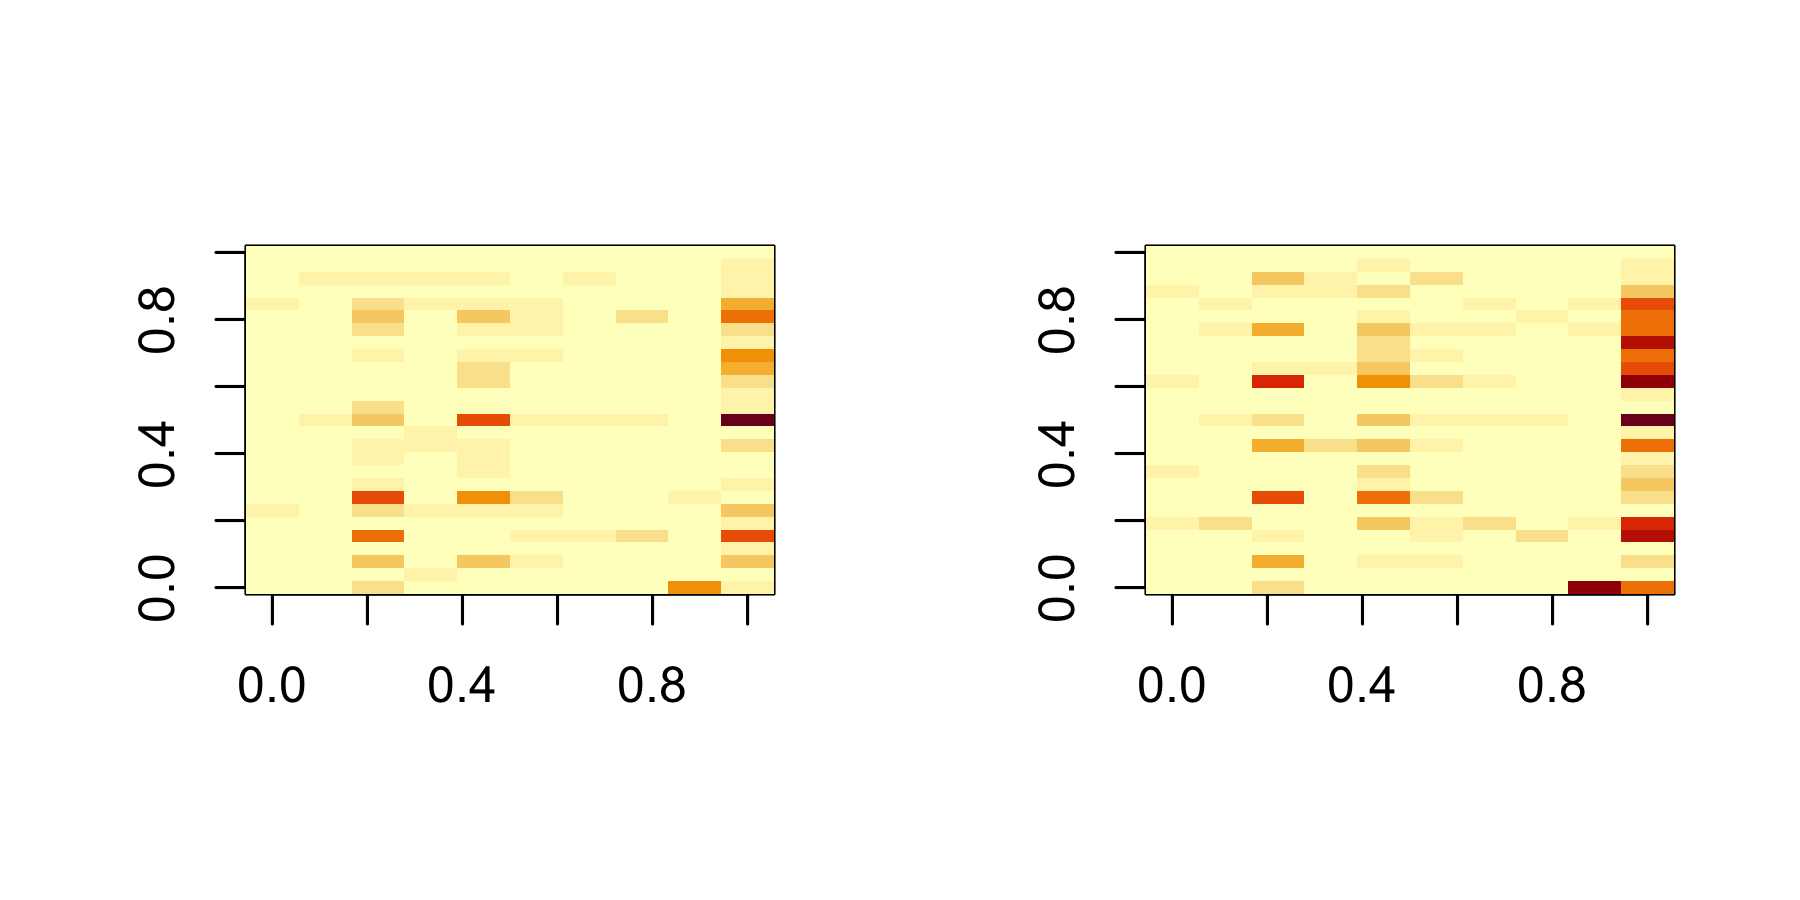
\includegraphics[width=\textwidth]{figure_roo_summary/Bone-Osteosarc_signatures_ROOcount_matrices_active.png}\end{minipage}\begin{minipage}{.24\textwidth}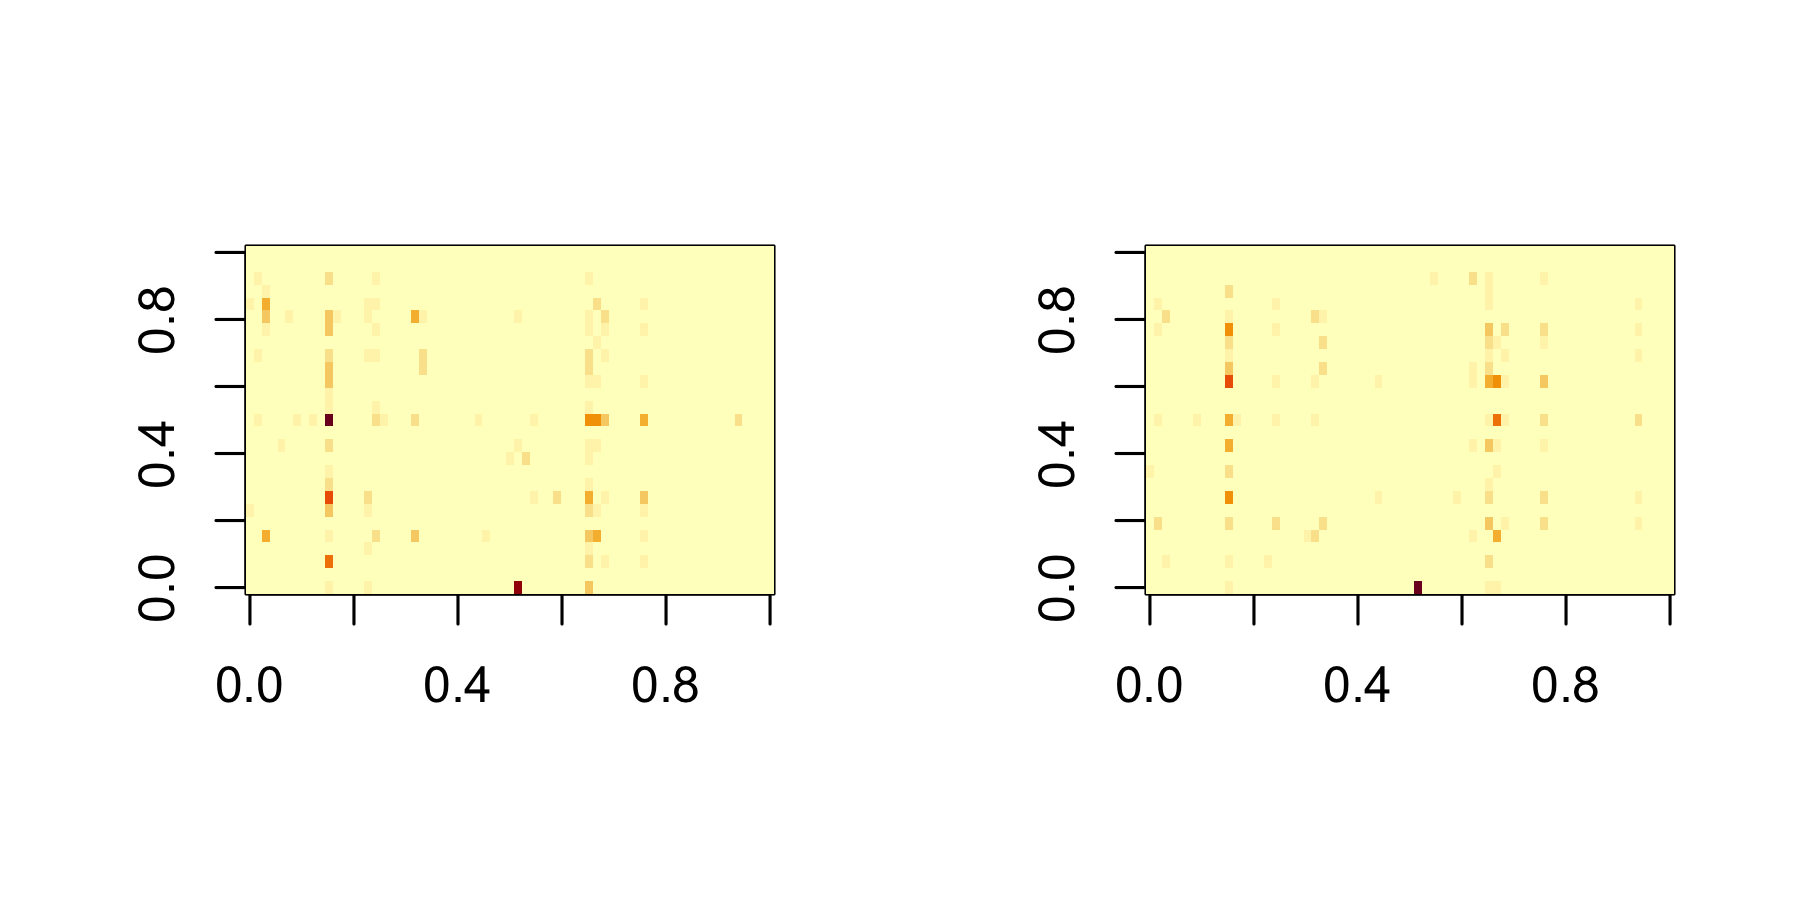
\includegraphics[width=\textwidth]{figure_roo_summary/Bone-Osteosarc_signatures_ROOcount_matrices_all.png}\end{minipage}\caption{Bone-Osteosarc}\end{figure}\begin{figure}\begin{minipage}{.24\textwidth}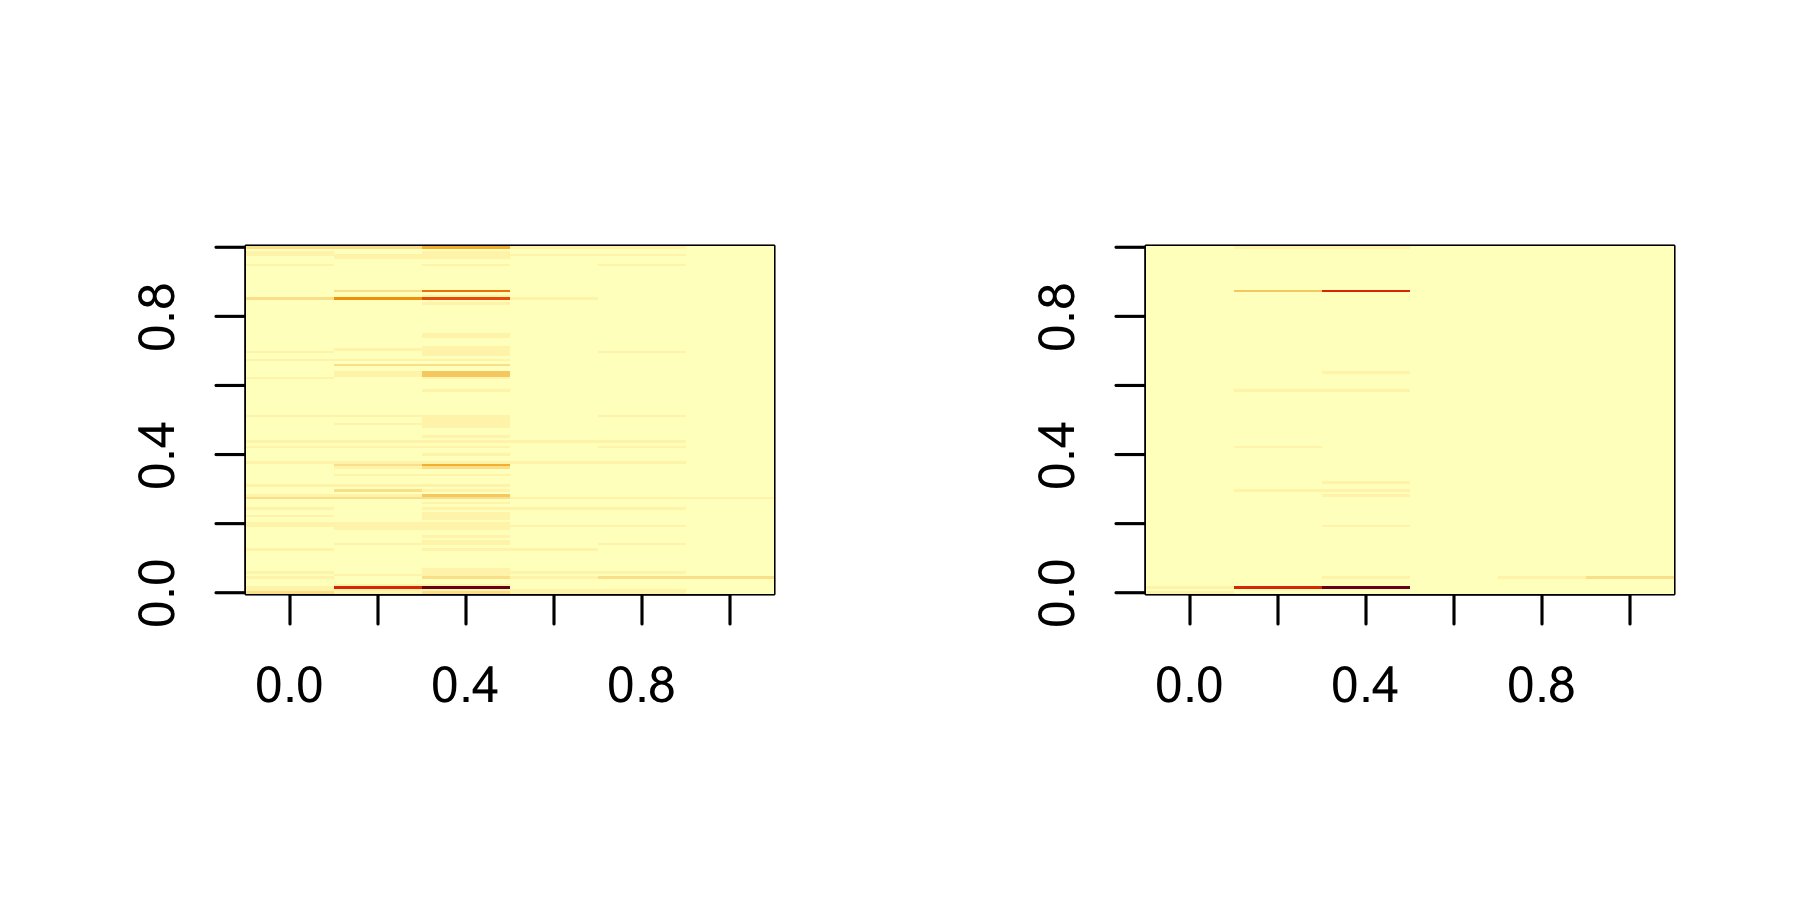
\includegraphics[width=\textwidth]{figure_roo_summary/Breast-AdenoCA_nucleotidesubstitution1_ROOcount_matrices_all.png}\end{minipage}\begin{minipage}{.24\textwidth}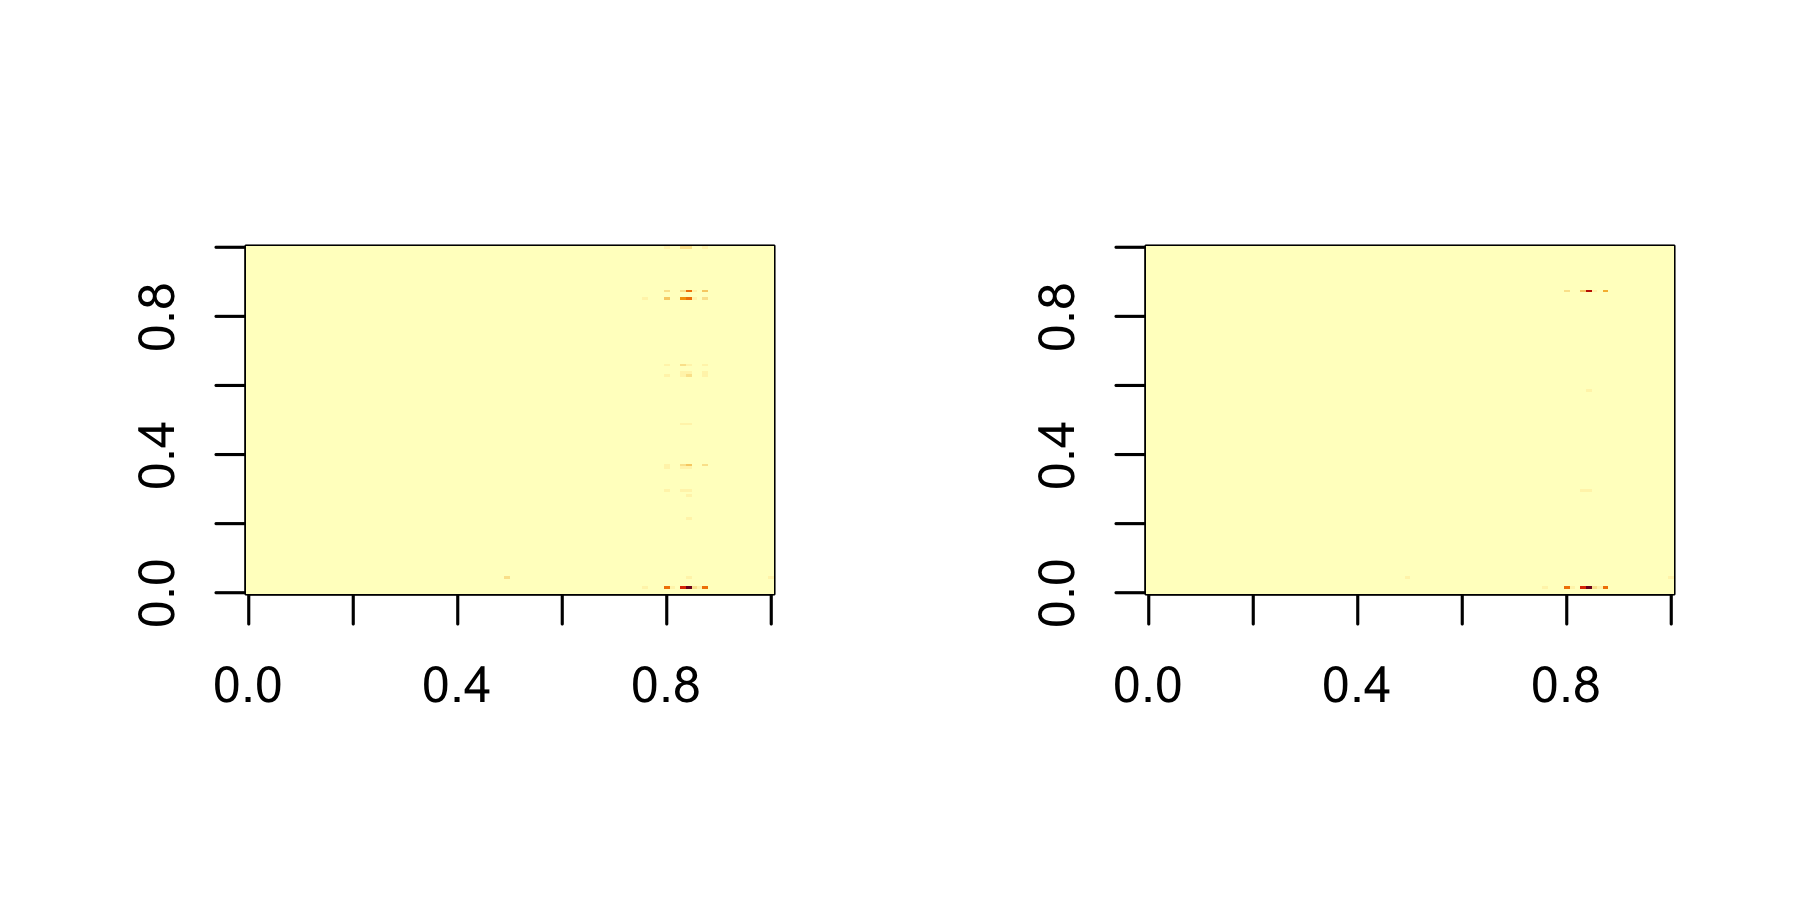
\includegraphics[width=\textwidth]{figure_roo_summary/Breast-AdenoCA_nucleotidesubstitution3_ROOcount_matrices_all.png}\end{minipage}\begin{minipage}{.24\textwidth}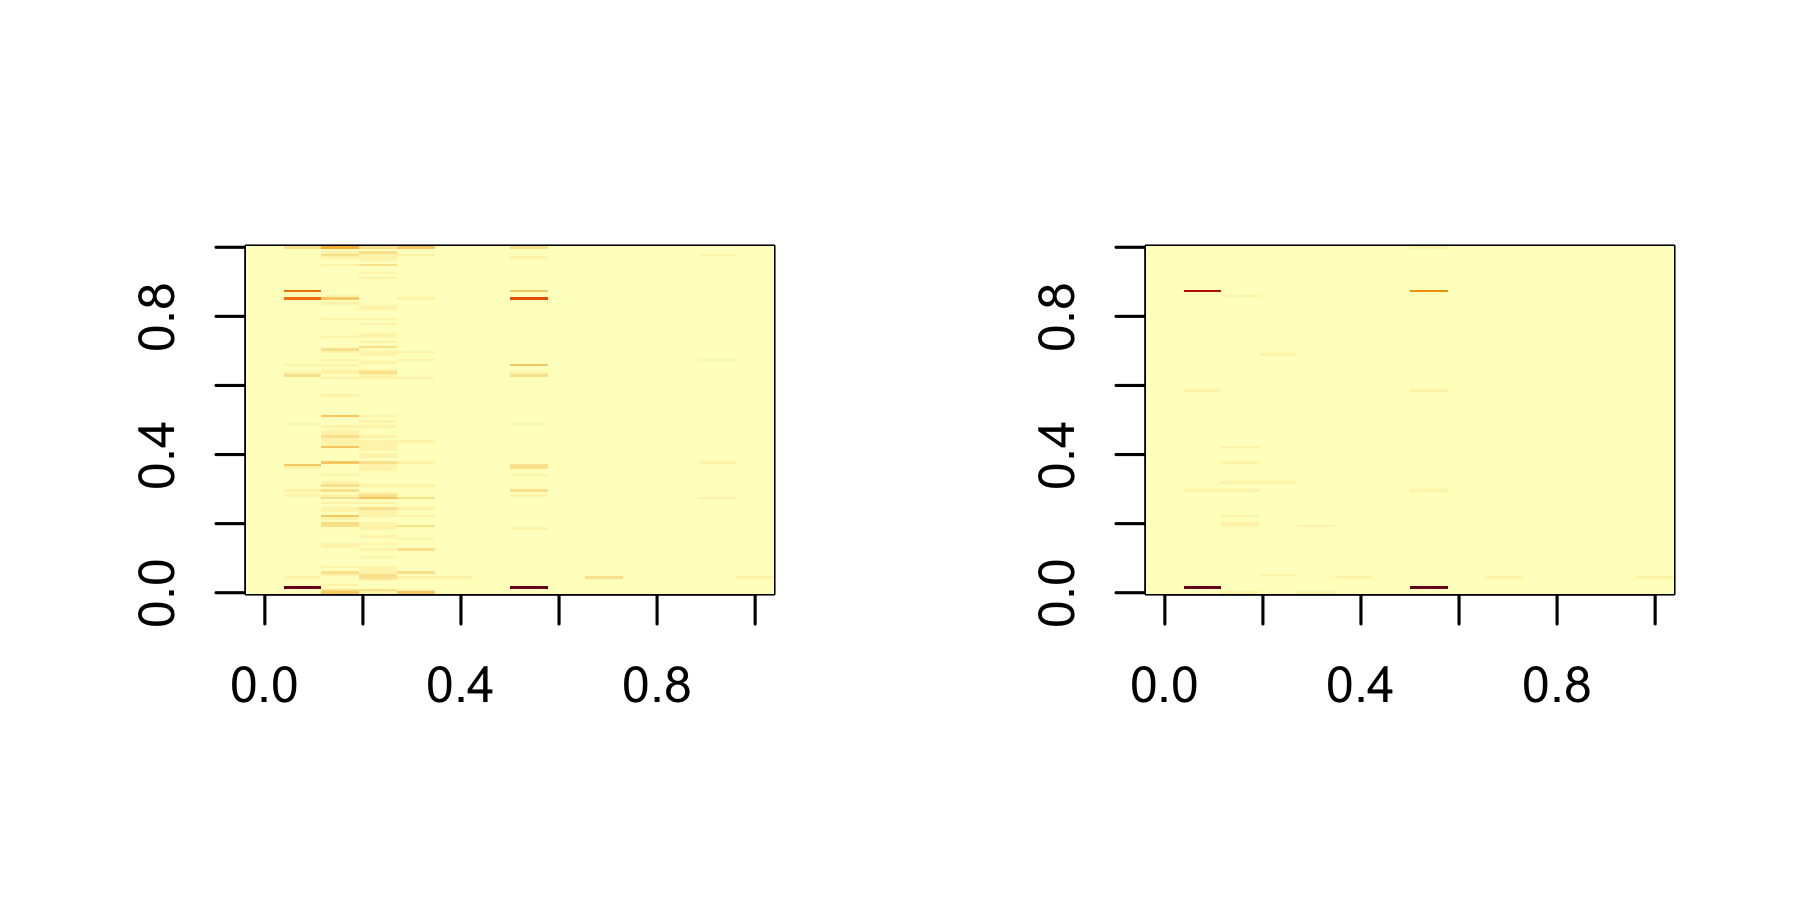
\includegraphics[width=\textwidth]{figure_roo_summary/Breast-AdenoCA_signatures_ROOcount_matrices_active.png}\end{minipage}\begin{minipage}{.24\textwidth}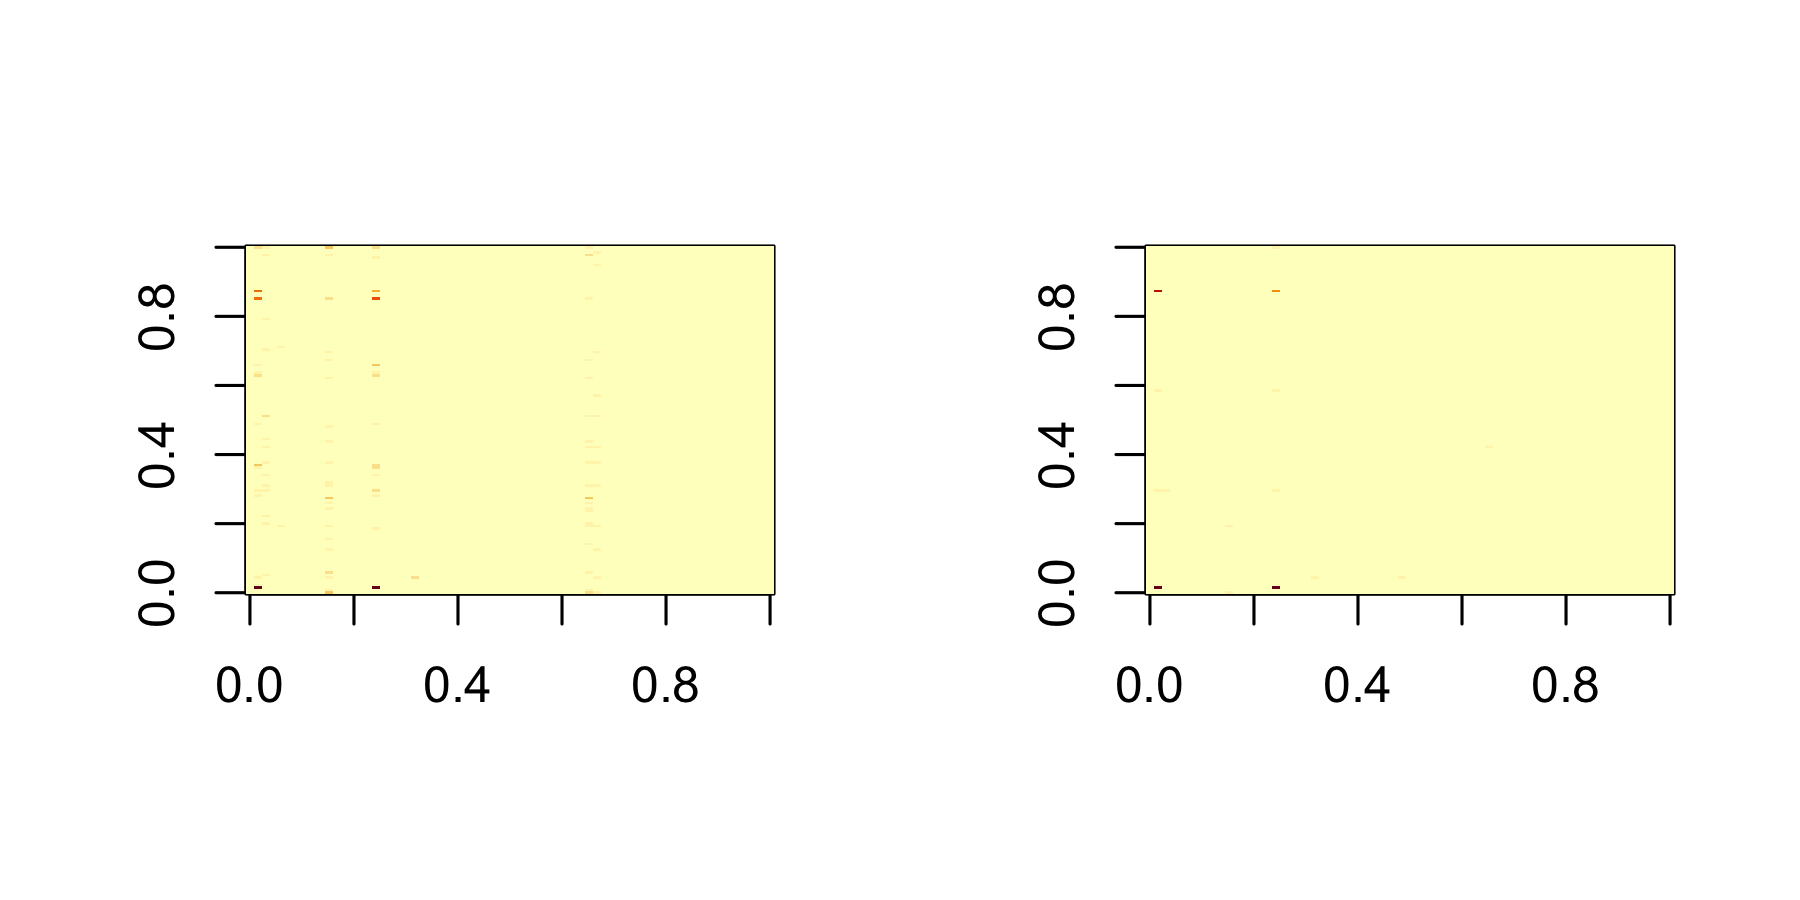
\includegraphics[width=\textwidth]{figure_roo_summary/Breast-AdenoCA_signatures_ROOcount_matrices_all.png}\end{minipage}\caption{Breast-AdenoCA}\end{figure}\begin{figure}\begin{minipage}{.24\textwidth}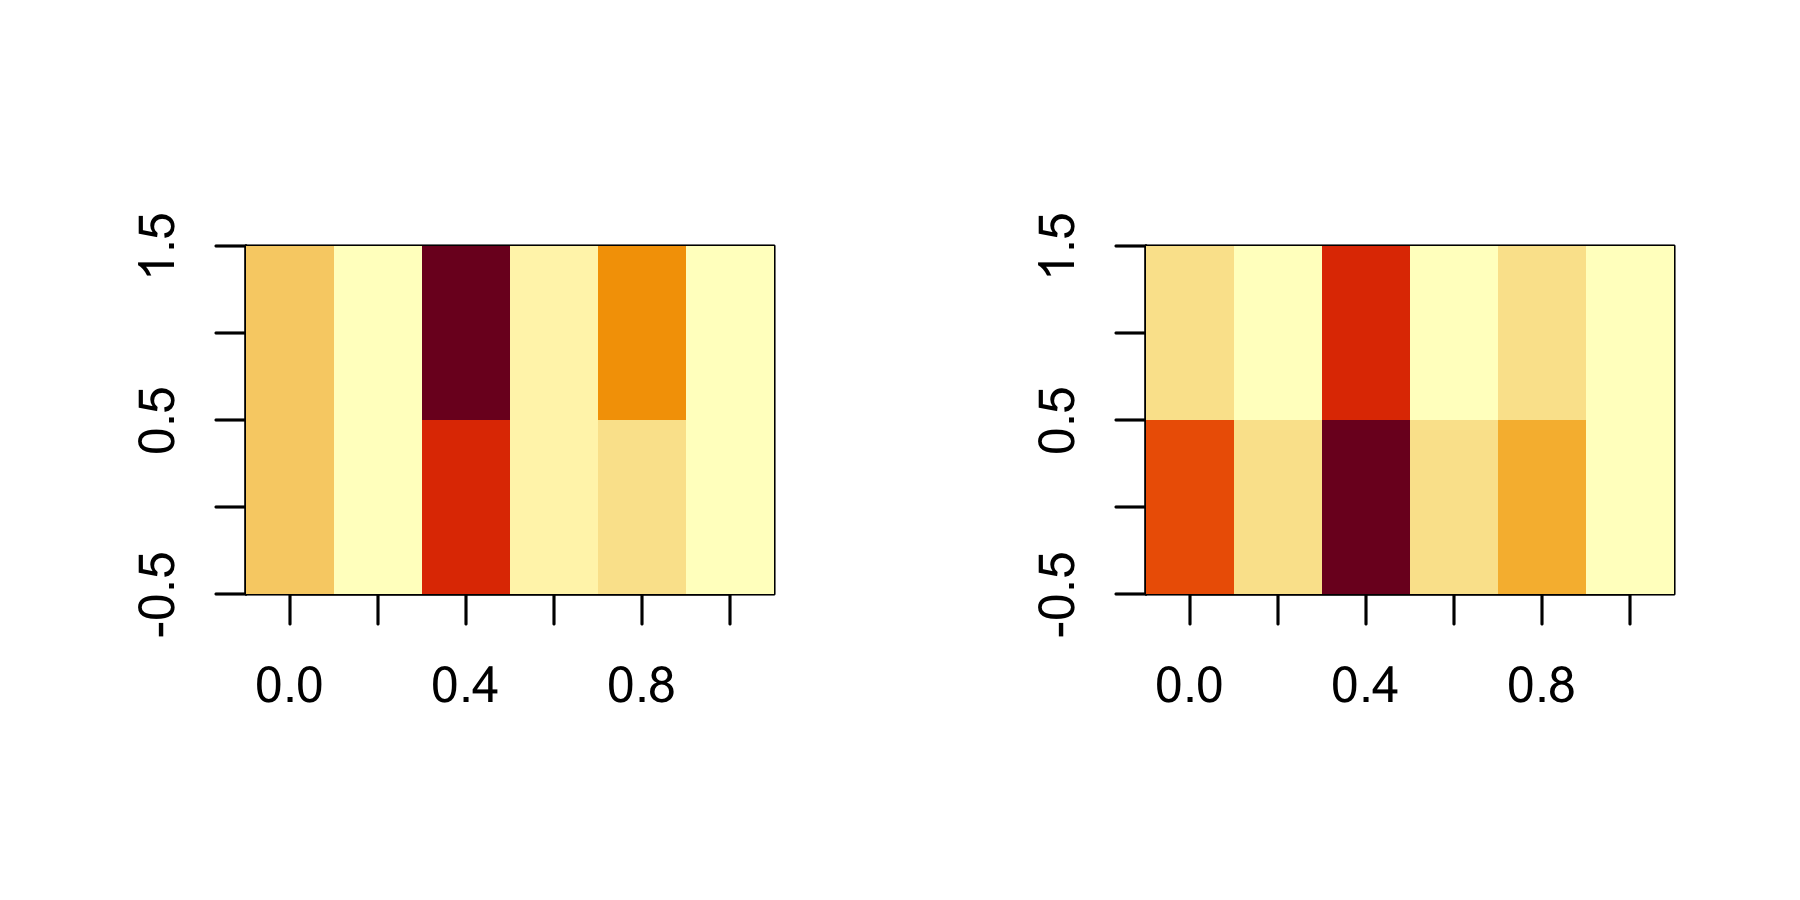
\includegraphics[width=\textwidth]{figure_roo_summary/Breast-DCIS_nucleotidesubstitution1_ROOcount_matrices_all.png}\end{minipage}\begin{minipage}{.24\textwidth}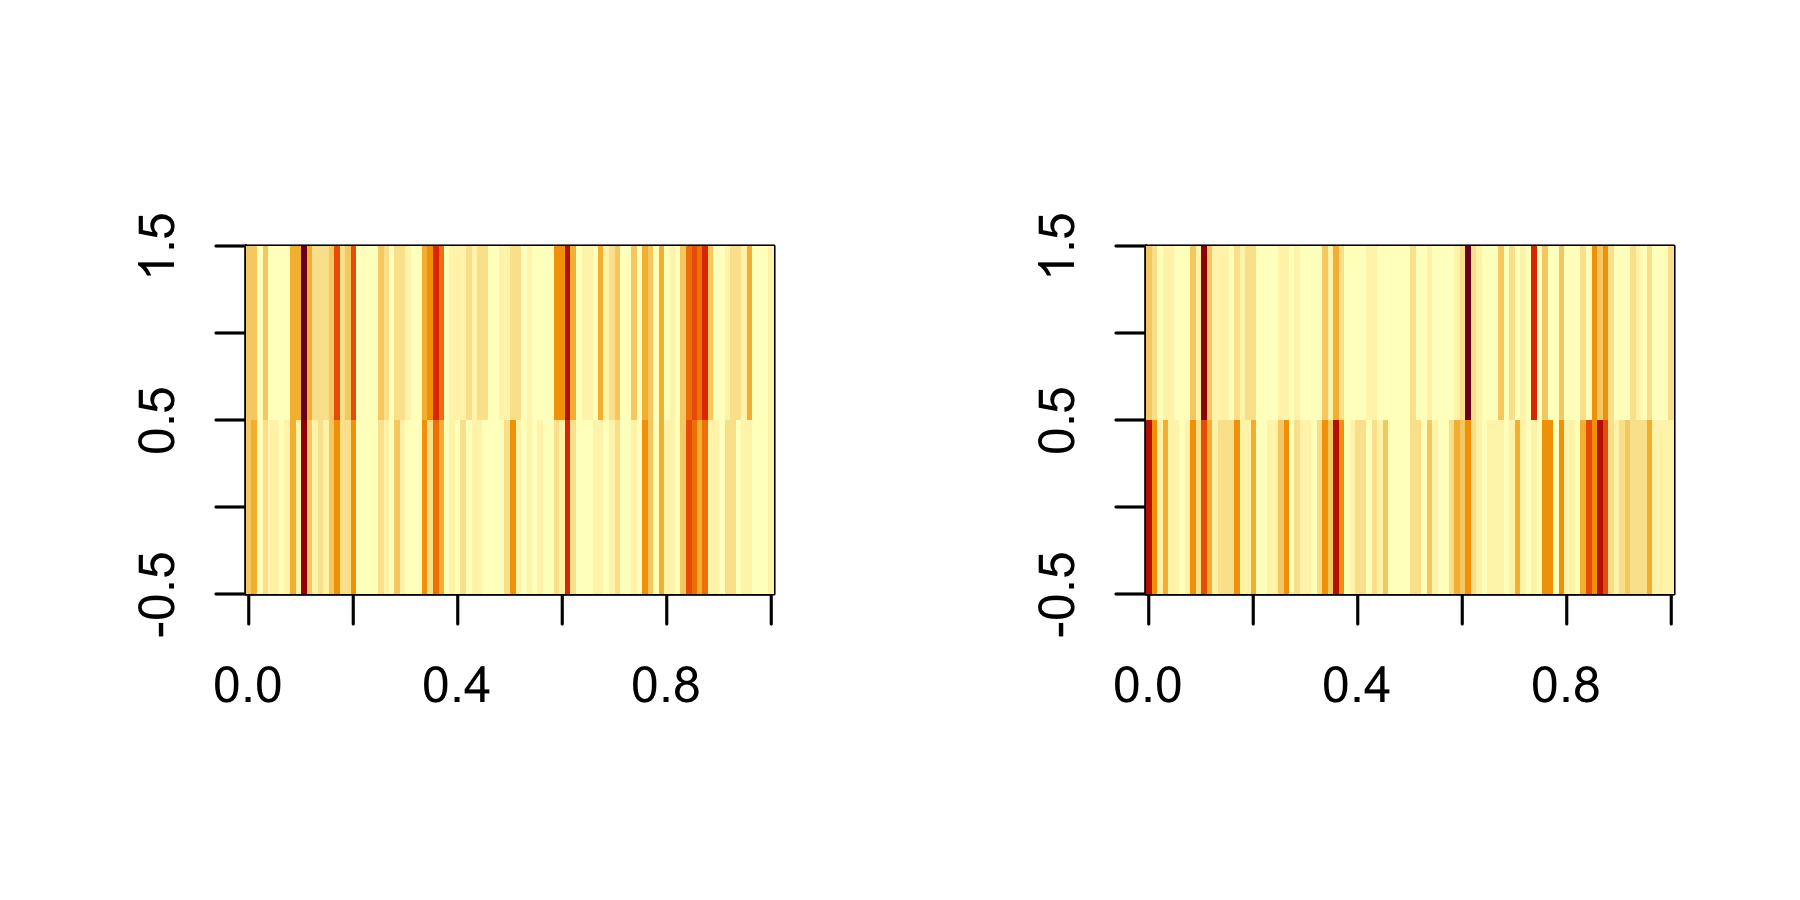
\includegraphics[width=\textwidth]{figure_roo_summary/Breast-DCIS_nucleotidesubstitution3_ROOcount_matrices_all.png}\end{minipage}\begin{minipage}{.24\textwidth}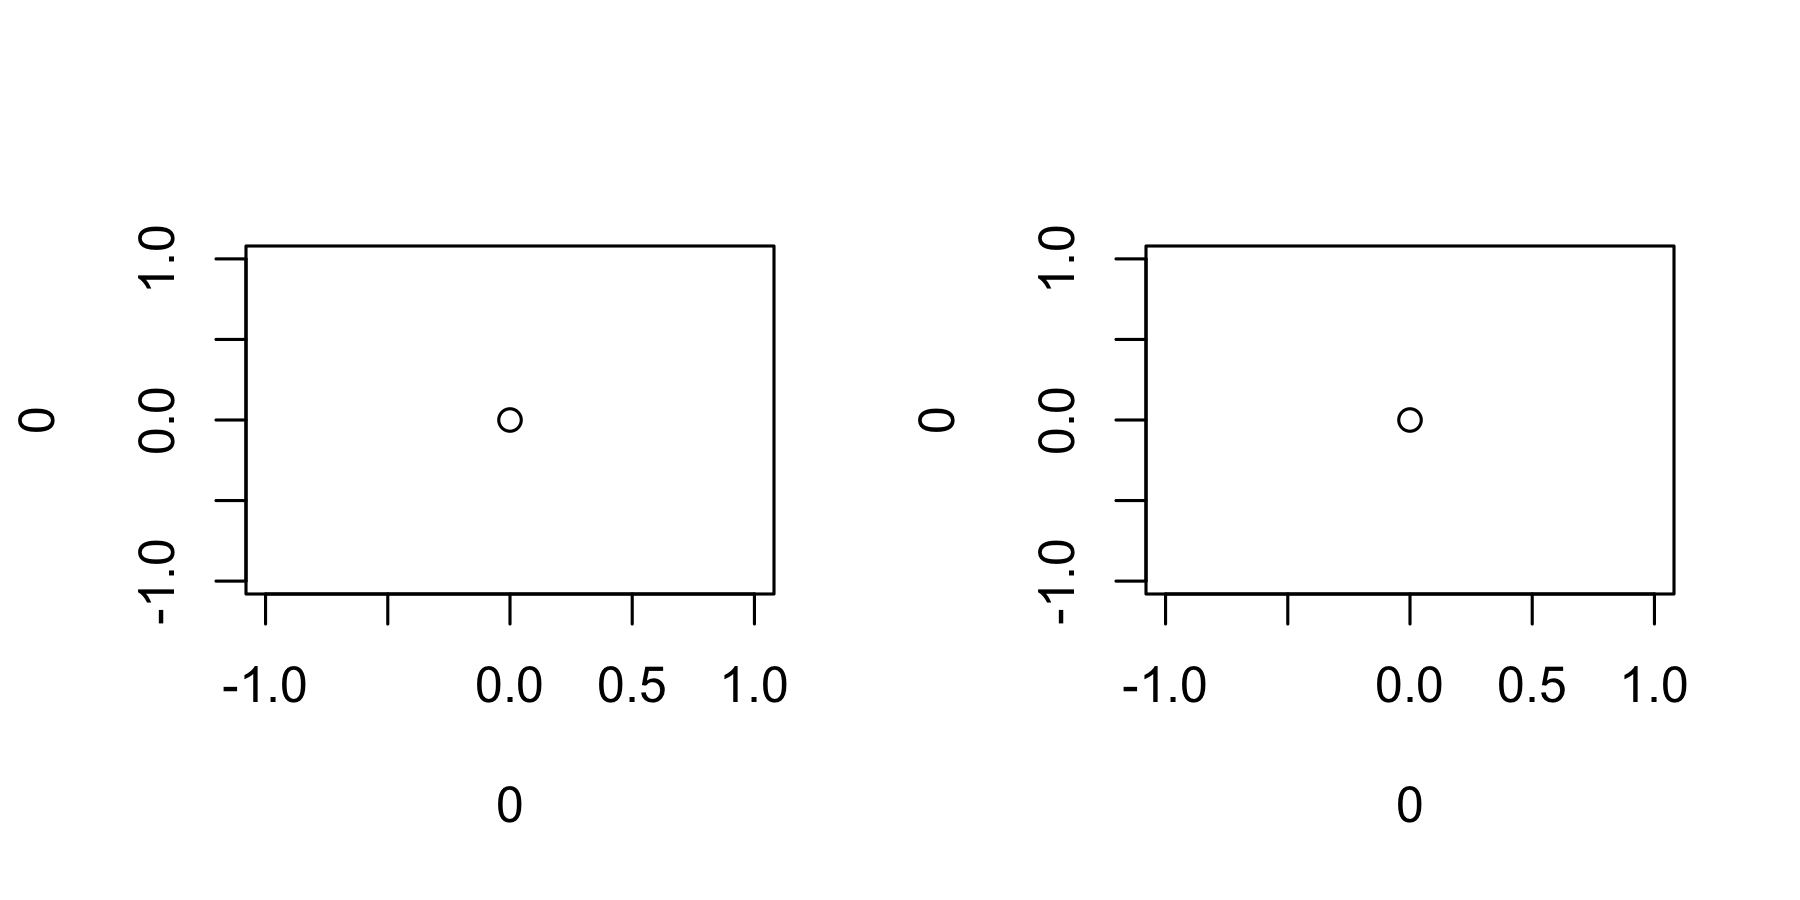
\includegraphics[width=\textwidth]{figure_roo_summary/Breast-DCIS_signatures_ROOcount_matrices_active.png}\end{minipage}\begin{minipage}{.24\textwidth}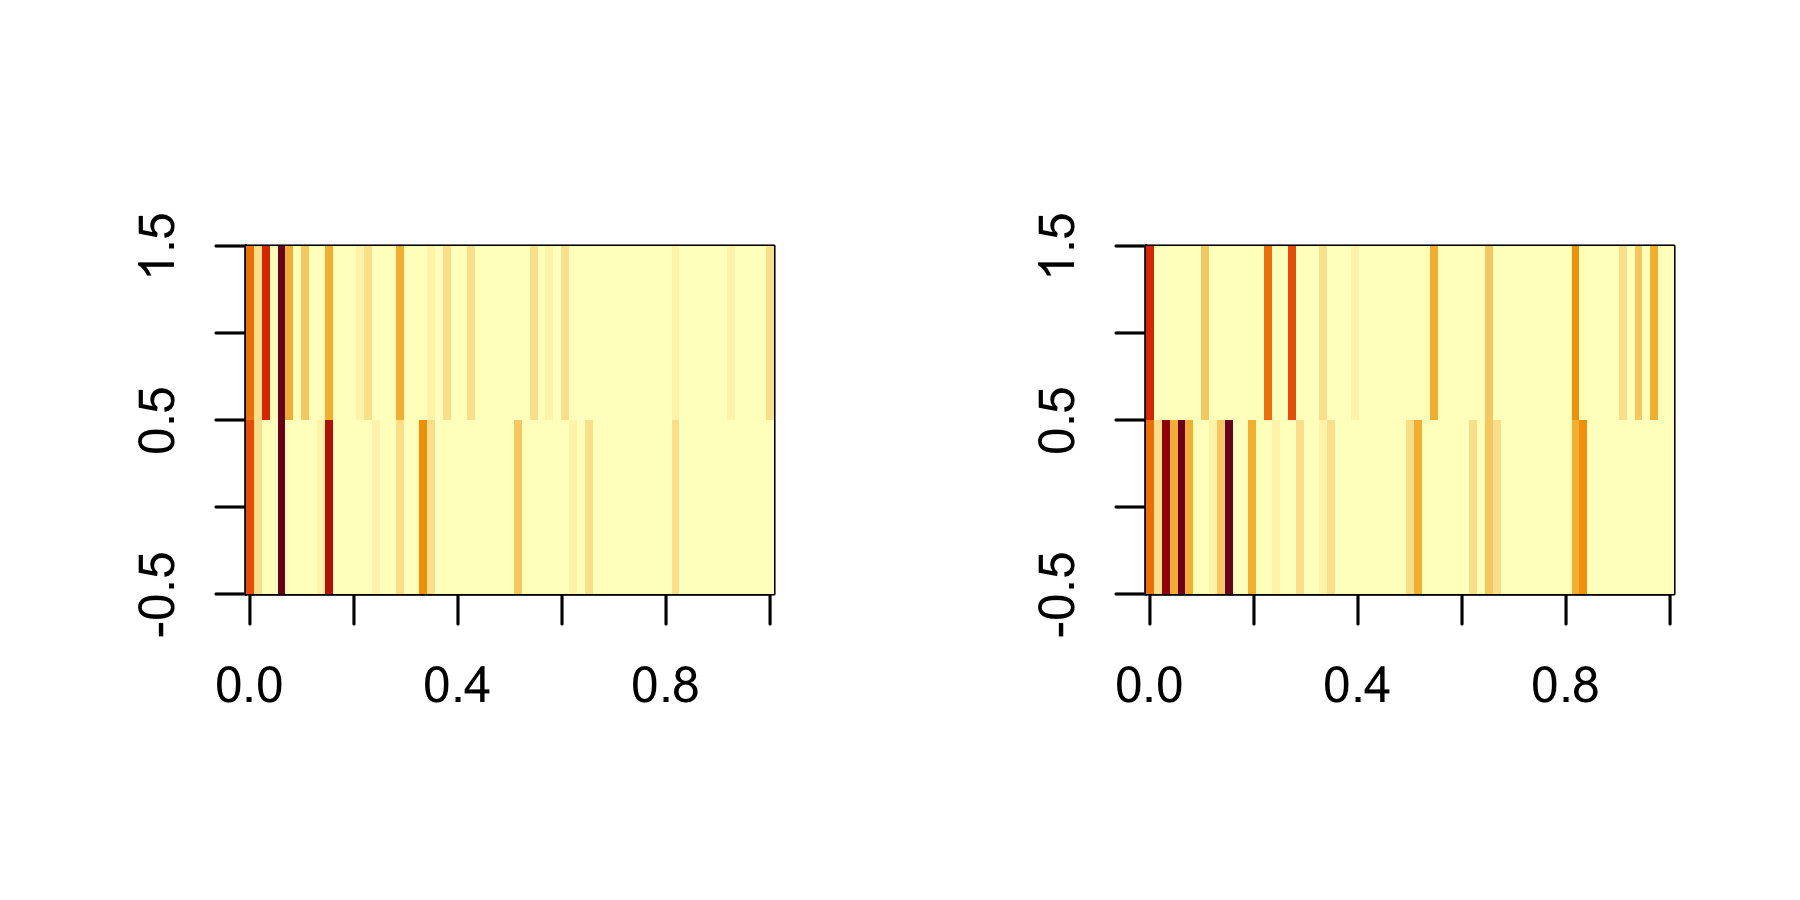
\includegraphics[width=\textwidth]{figure_roo_summary/Breast-DCIS_signatures_ROOcount_matrices_all.png}\end{minipage}\caption{Breast-DCIS}\end{figure}\begin{figure}\begin{minipage}{.24\textwidth}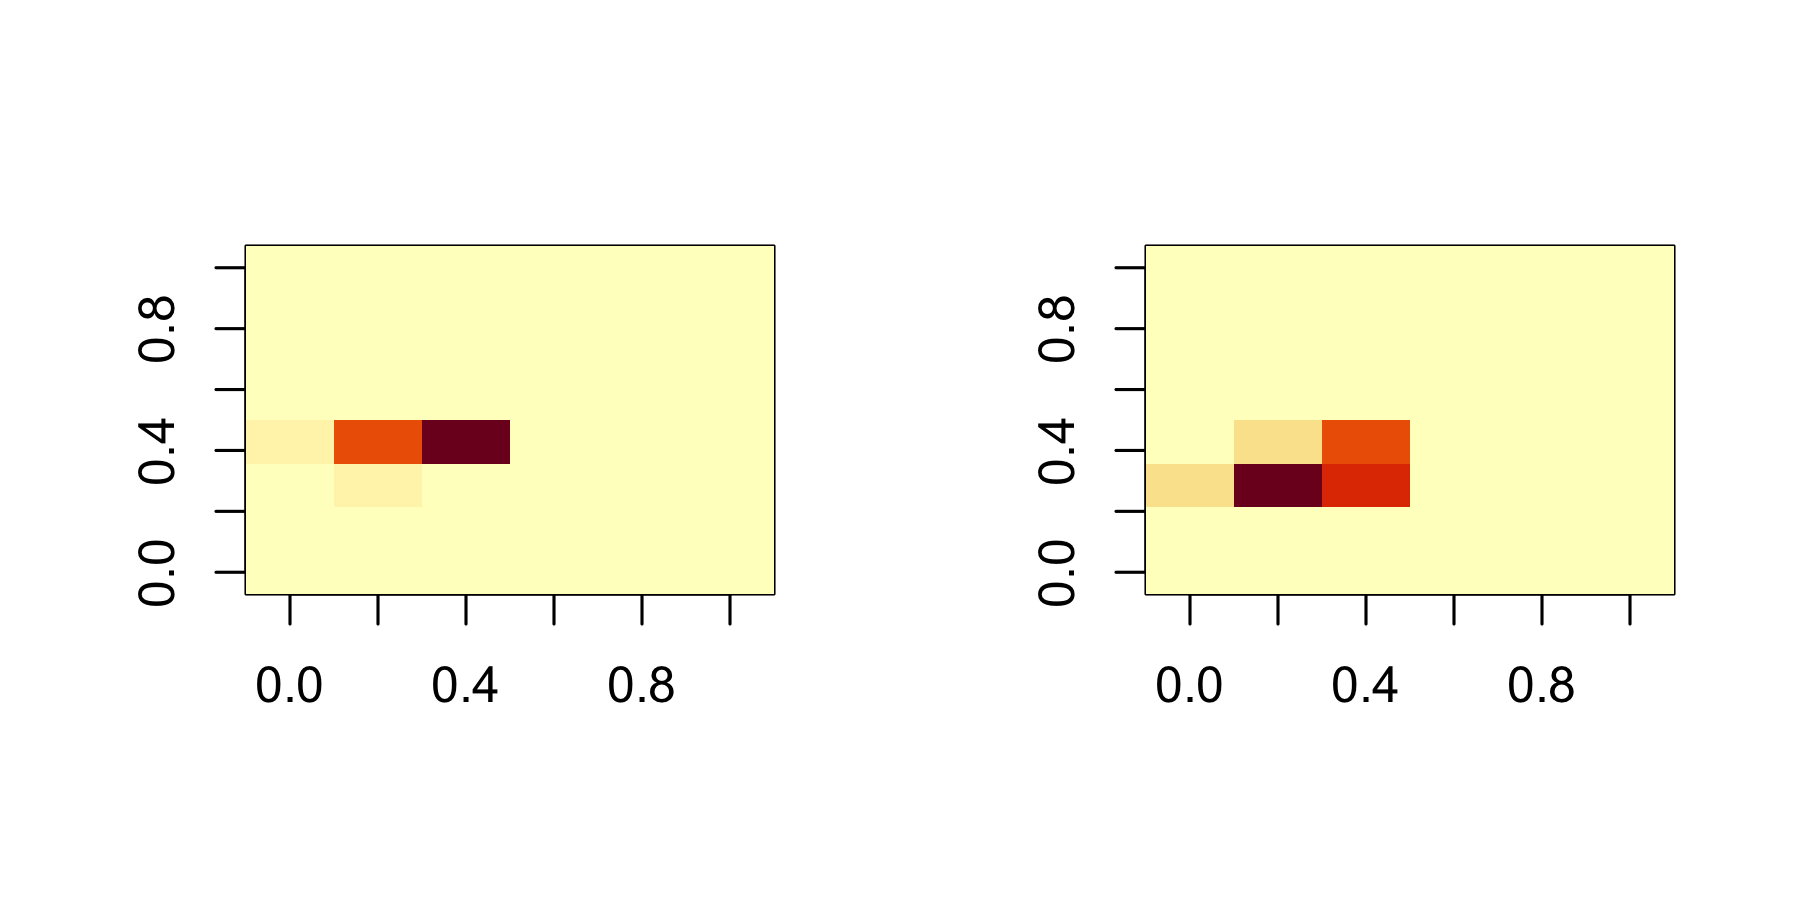
\includegraphics[width=\textwidth]{figure_roo_summary/Breast-LobularCA_nucleotidesubstitution1_ROOcount_matrices_all.png}\end{minipage}\begin{minipage}{.24\textwidth}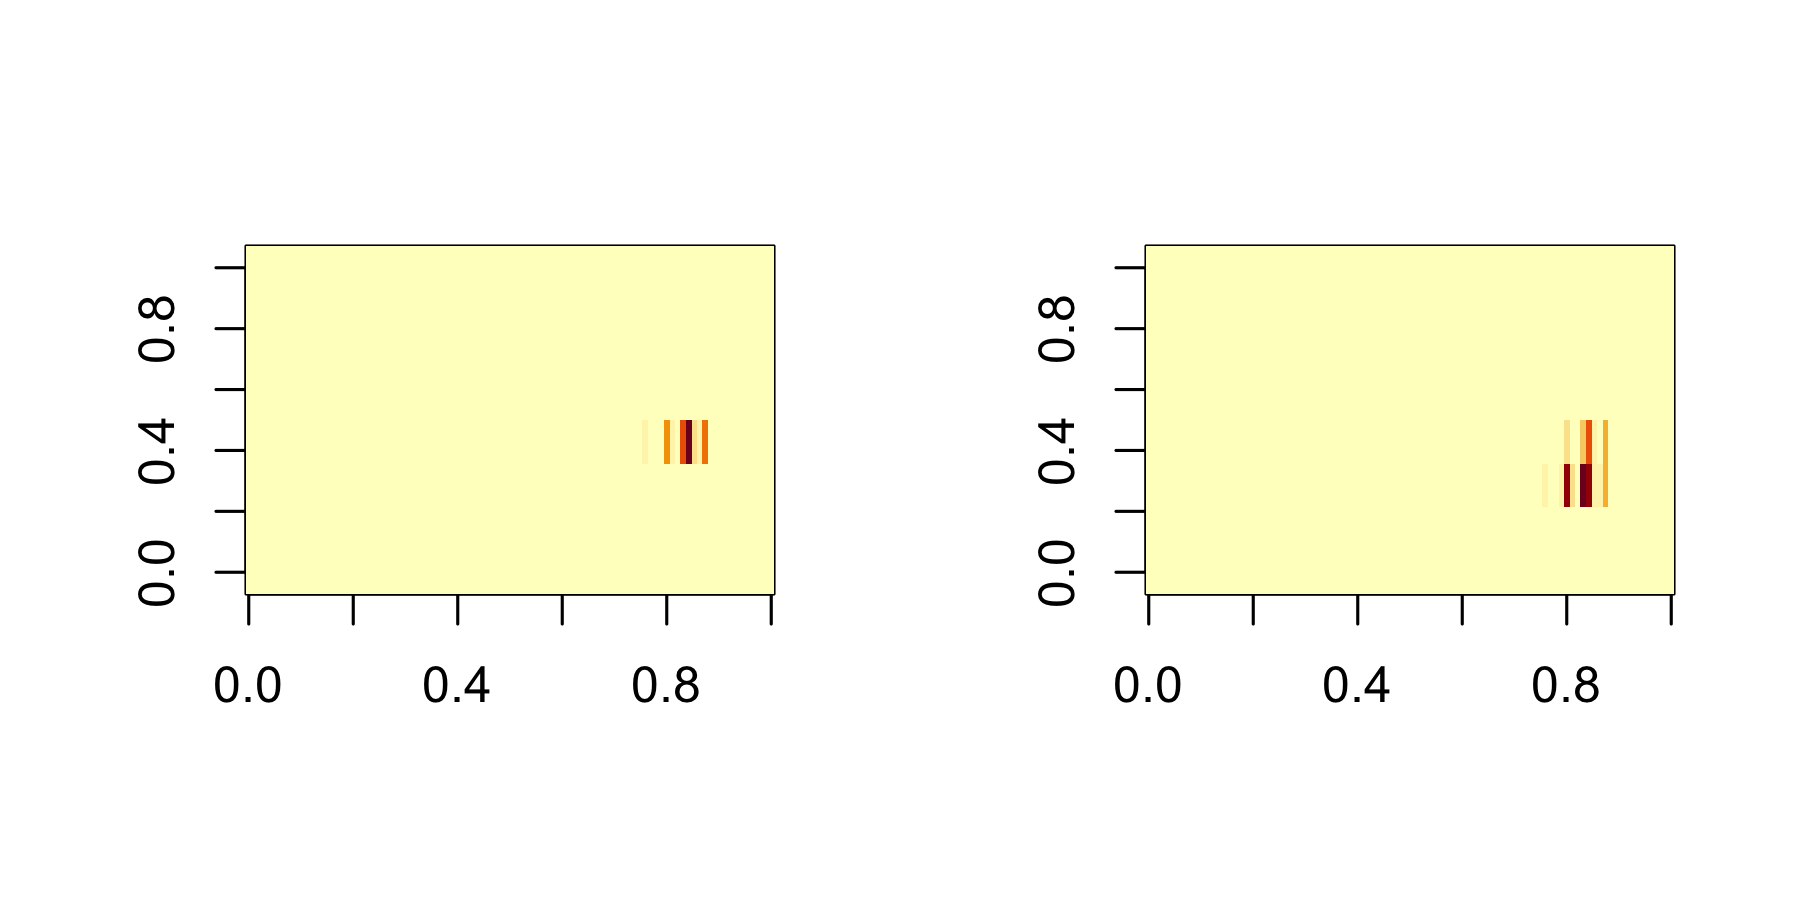
\includegraphics[width=\textwidth]{figure_roo_summary/Breast-LobularCA_nucleotidesubstitution3_ROOcount_matrices_all.png}\end{minipage}\begin{minipage}{.24\textwidth}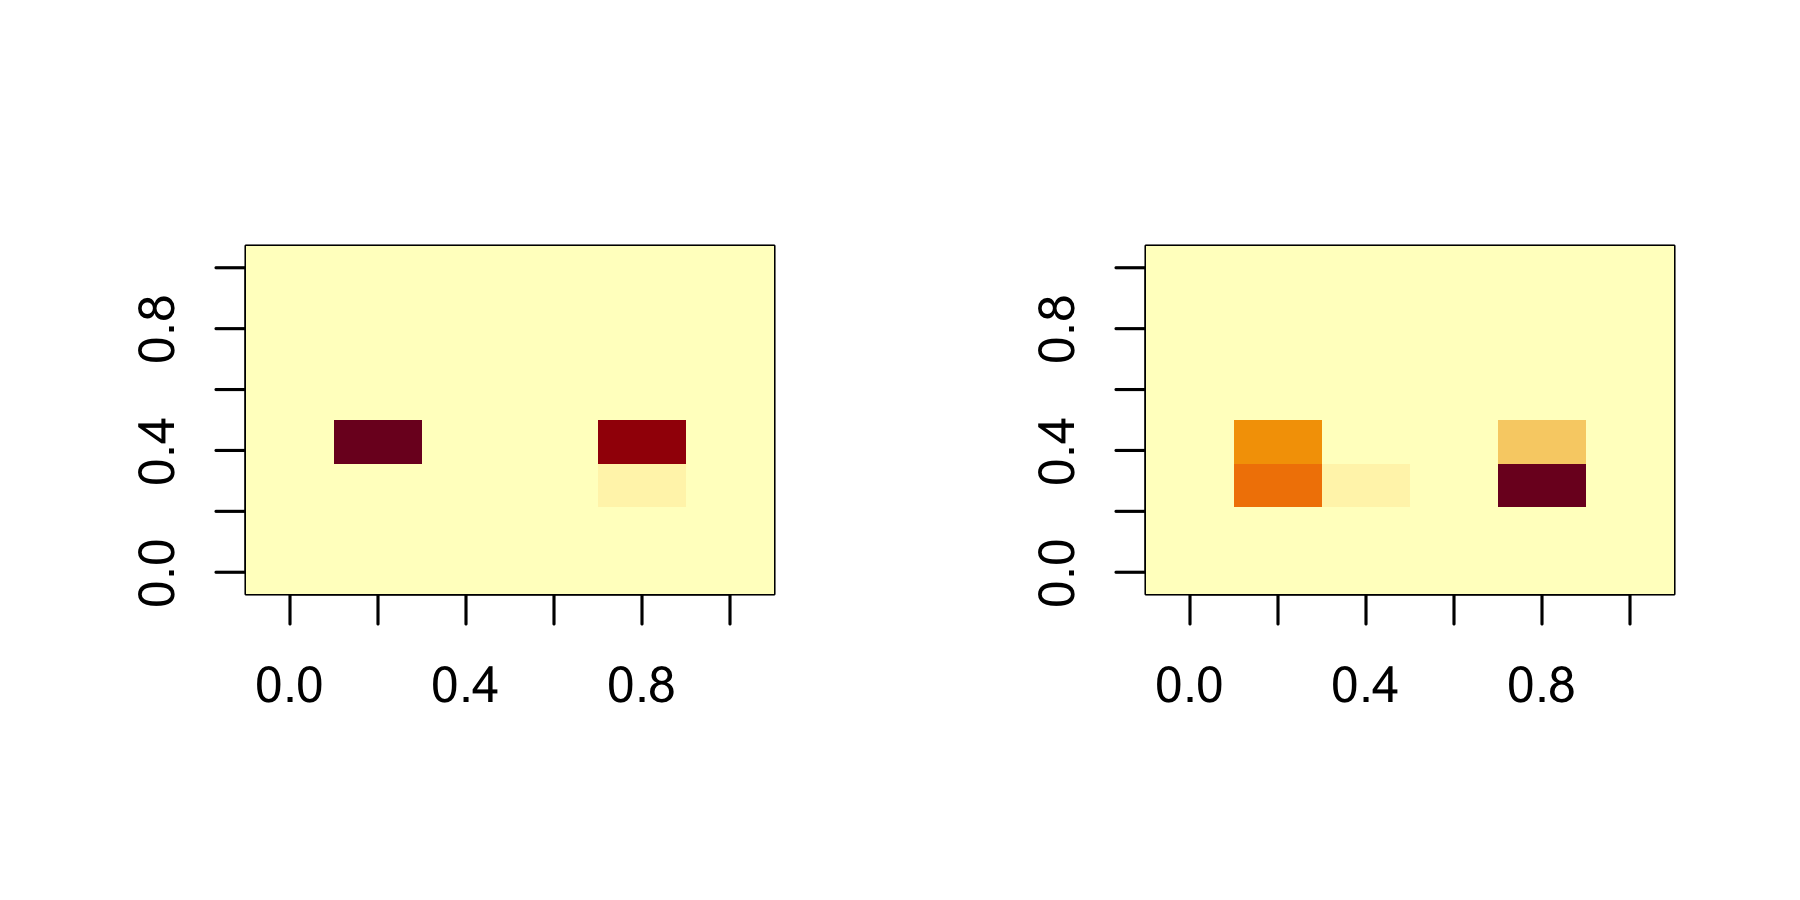
\includegraphics[width=\textwidth]{figure_roo_summary/Breast-LobularCA_signatures_ROOcount_matrices_active.png}\end{minipage}\begin{minipage}{.24\textwidth}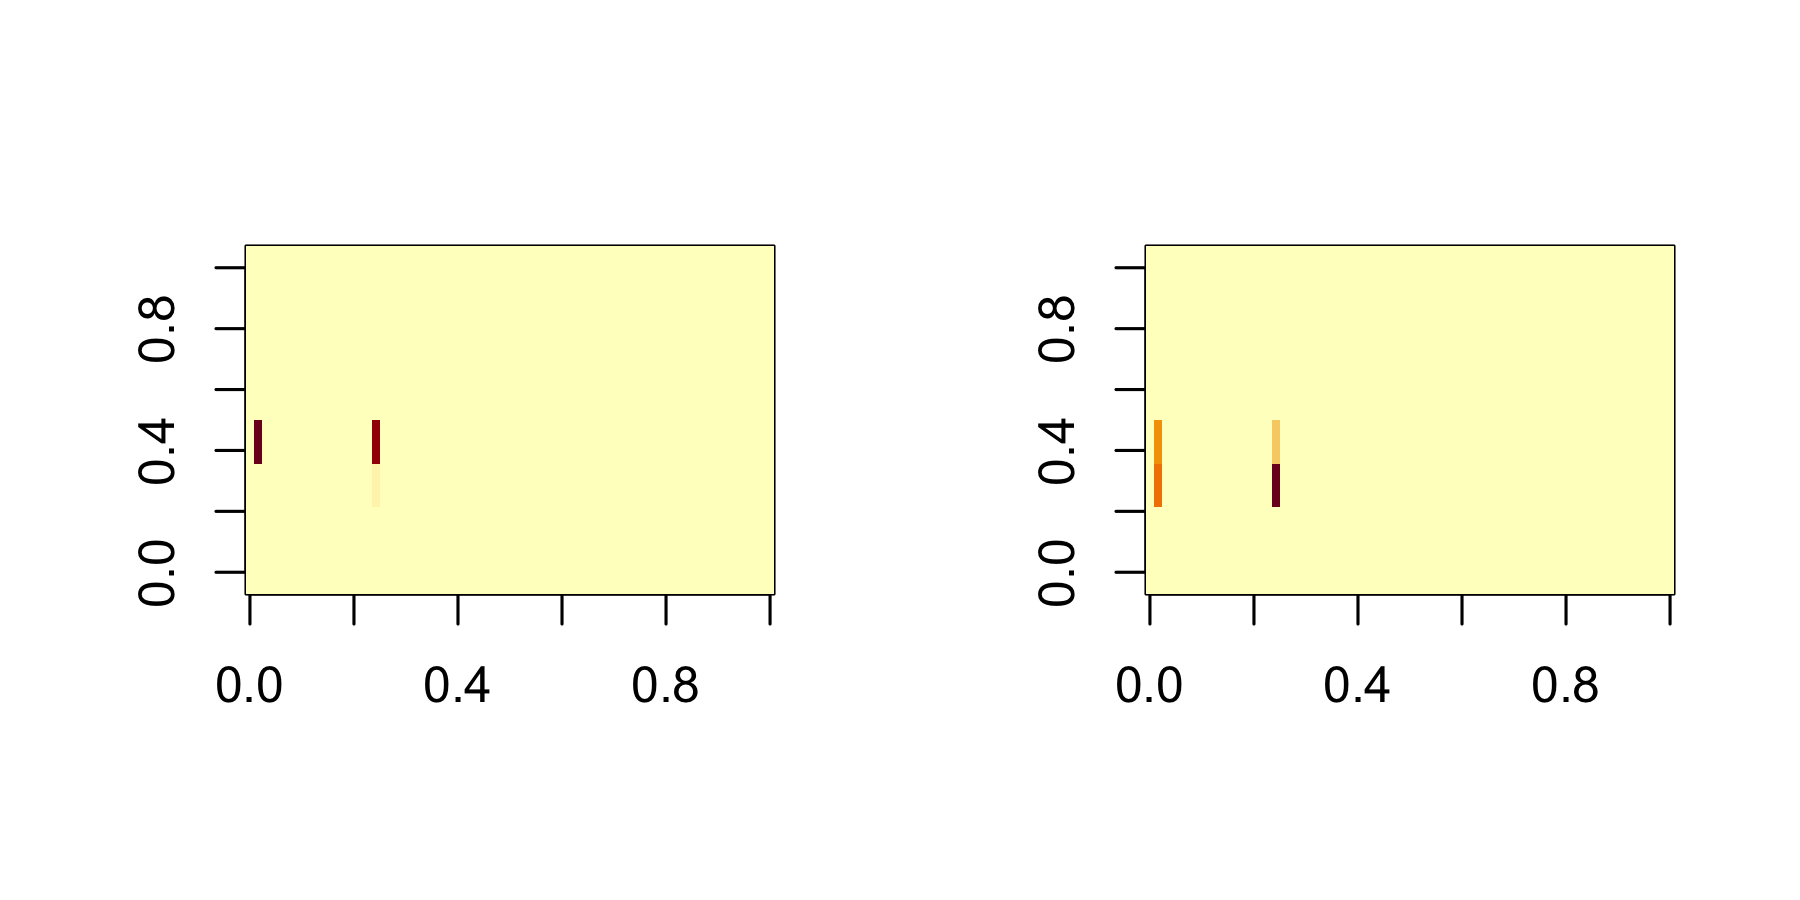
\includegraphics[width=\textwidth]{figure_roo_summary/Breast-LobularCA_signatures_ROOcount_matrices_all.png}\end{minipage}\caption{Breast-LobularCA}\end{figure}\begin{figure}\begin{minipage}{.24\textwidth}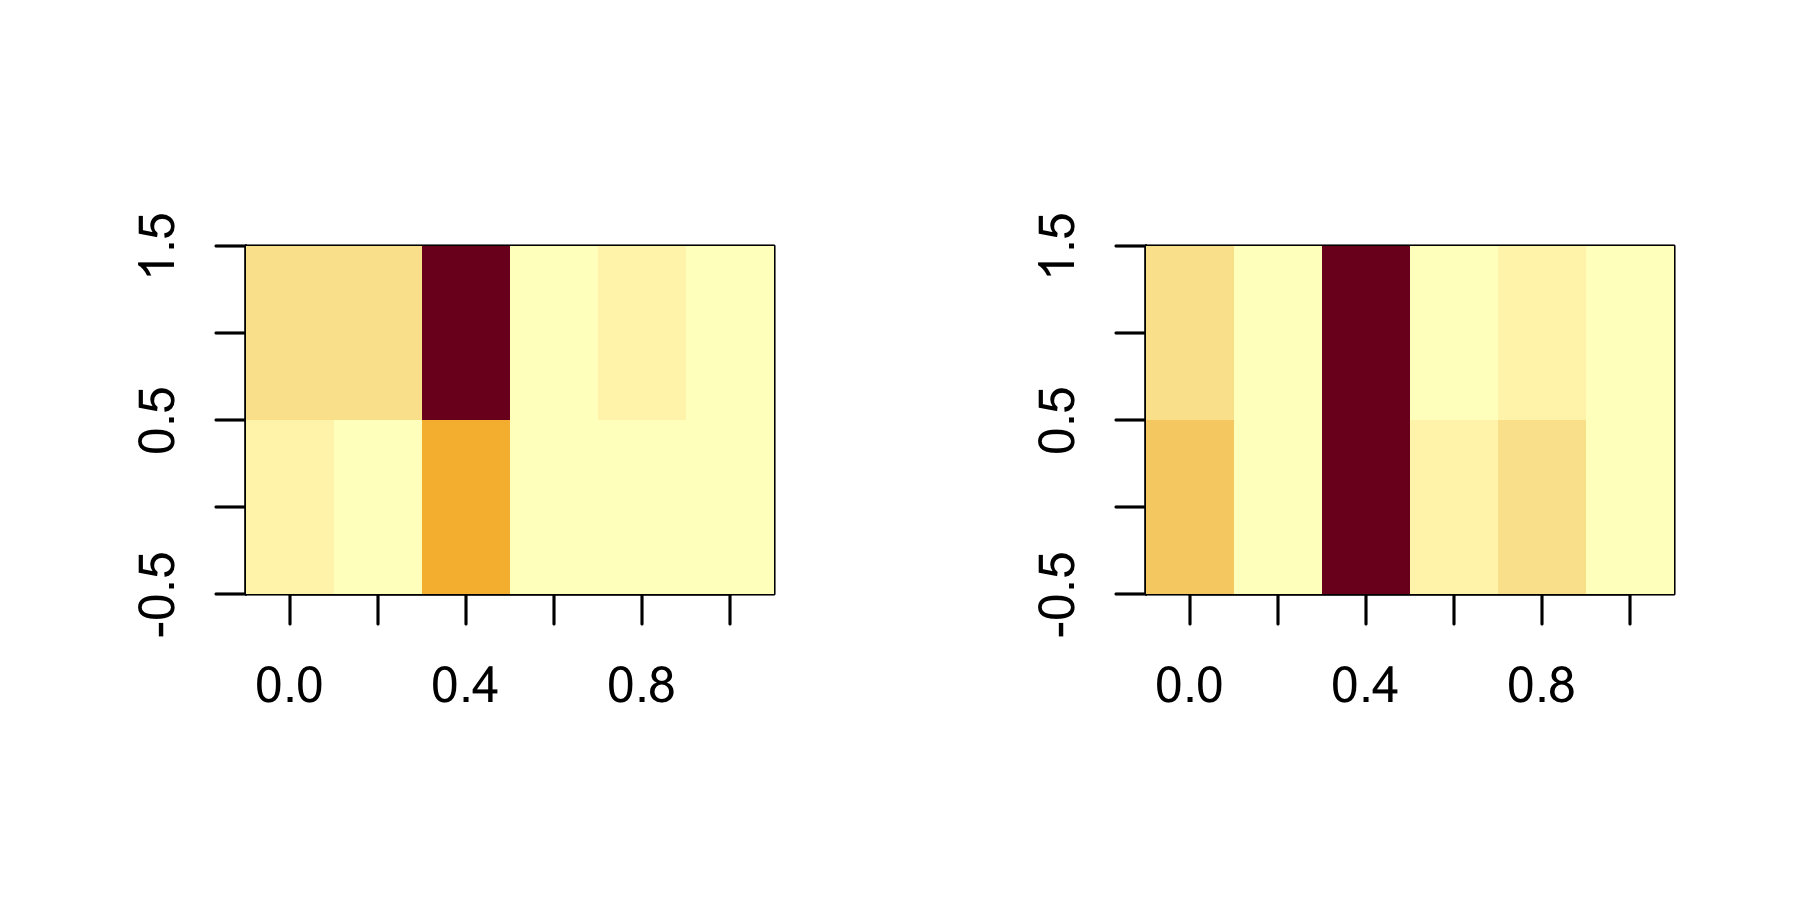
\includegraphics[width=\textwidth]{figure_roo_summary/Cervix-AdenoCA_nucleotidesubstitution1_ROOcount_matrices_all.png}\end{minipage}\begin{minipage}{.24\textwidth}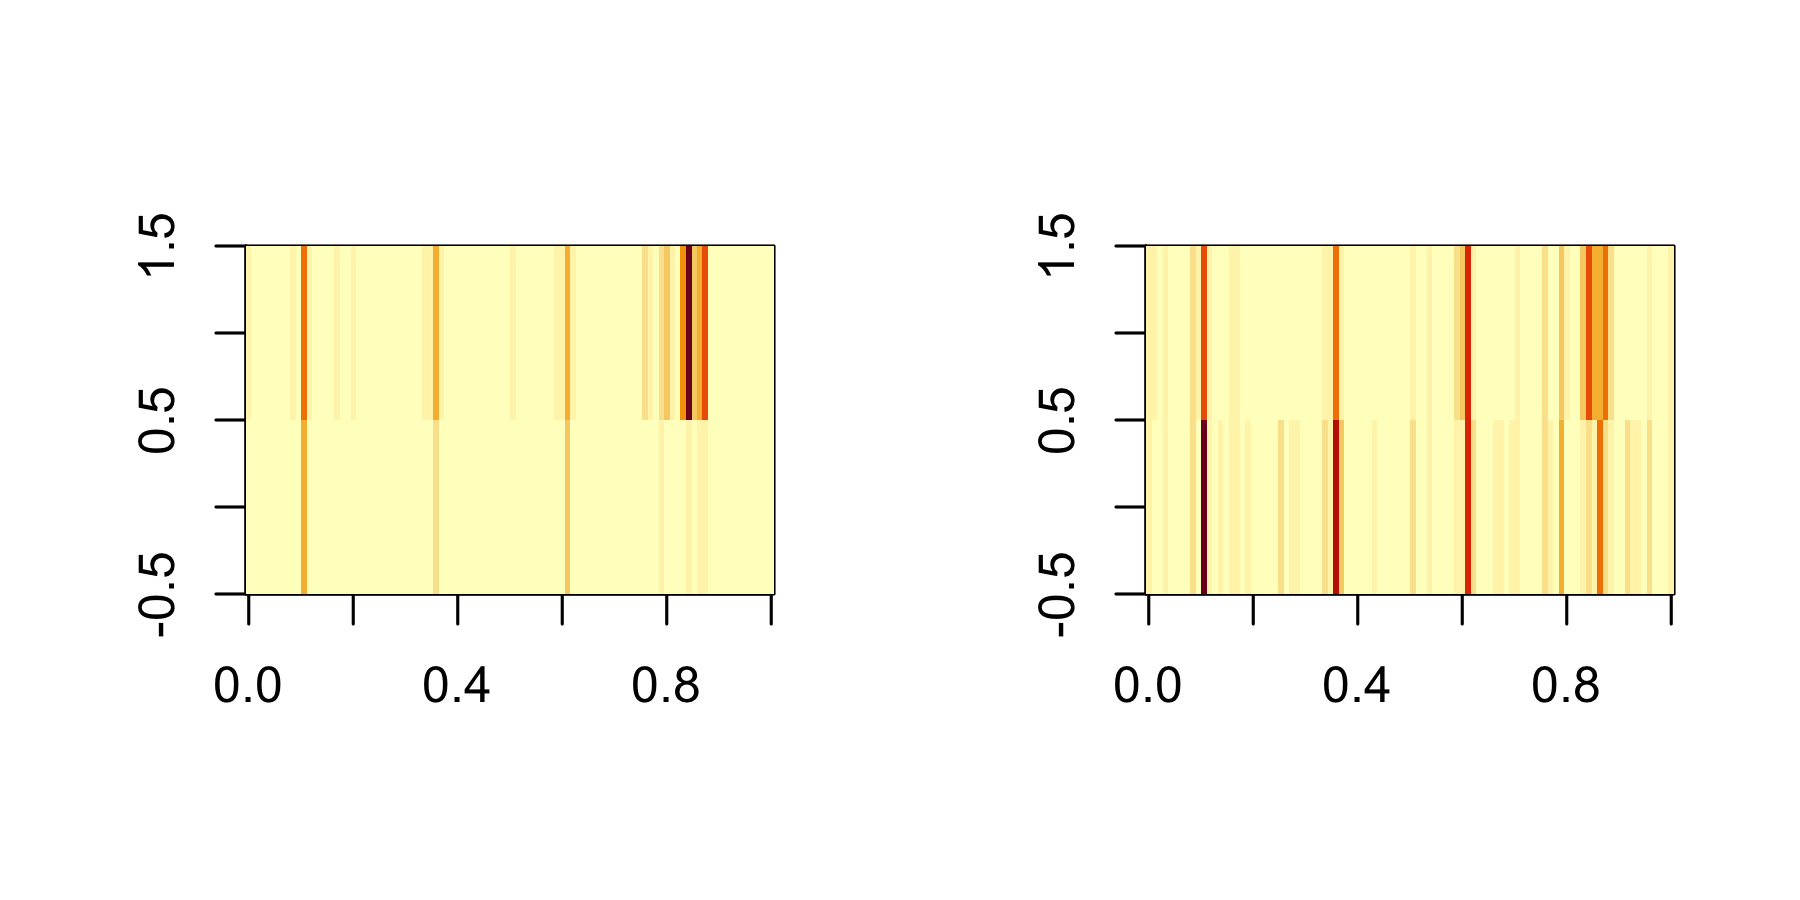
\includegraphics[width=\textwidth]{figure_roo_summary/Cervix-AdenoCA_nucleotidesubstitution3_ROOcount_matrices_all.png}\end{minipage}\begin{minipage}{.24\textwidth}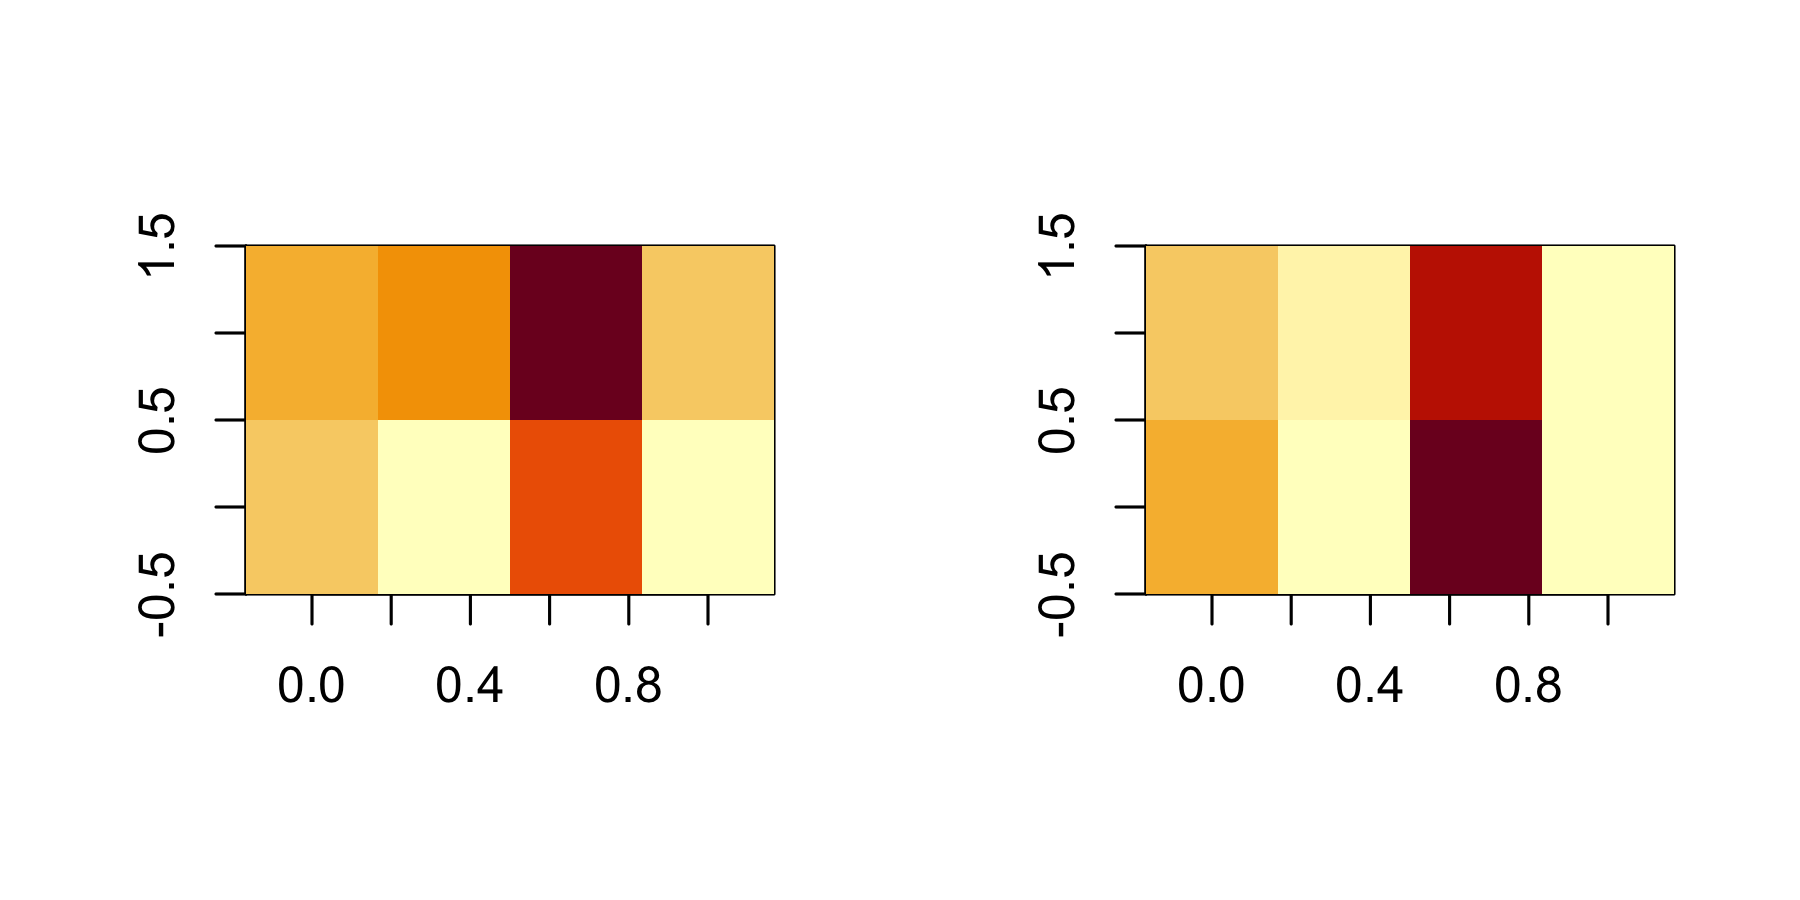
\includegraphics[width=\textwidth]{figure_roo_summary/Cervix-AdenoCA_signatures_ROOcount_matrices_active.png}\end{minipage}\begin{minipage}{.24\textwidth}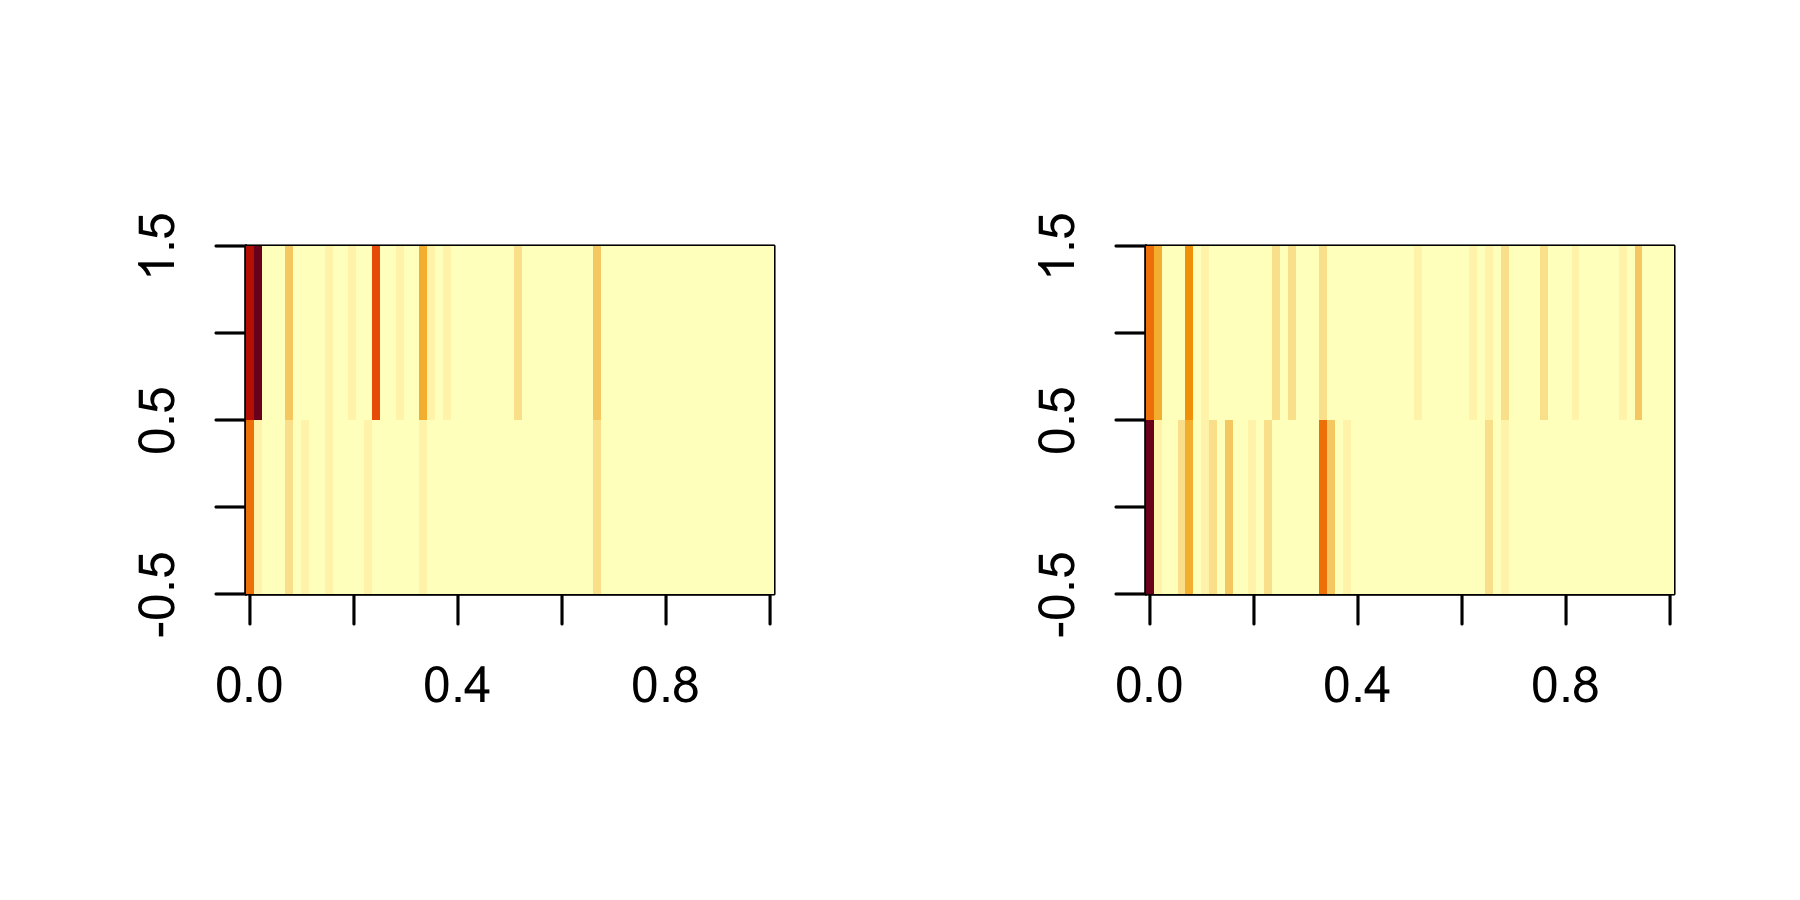
\includegraphics[width=\textwidth]{figure_roo_summary/Cervix-AdenoCA_signatures_ROOcount_matrices_all.png}\end{minipage}\caption{Cervix-AdenoCA}\end{figure}\begin{figure}\begin{minipage}{.24\textwidth}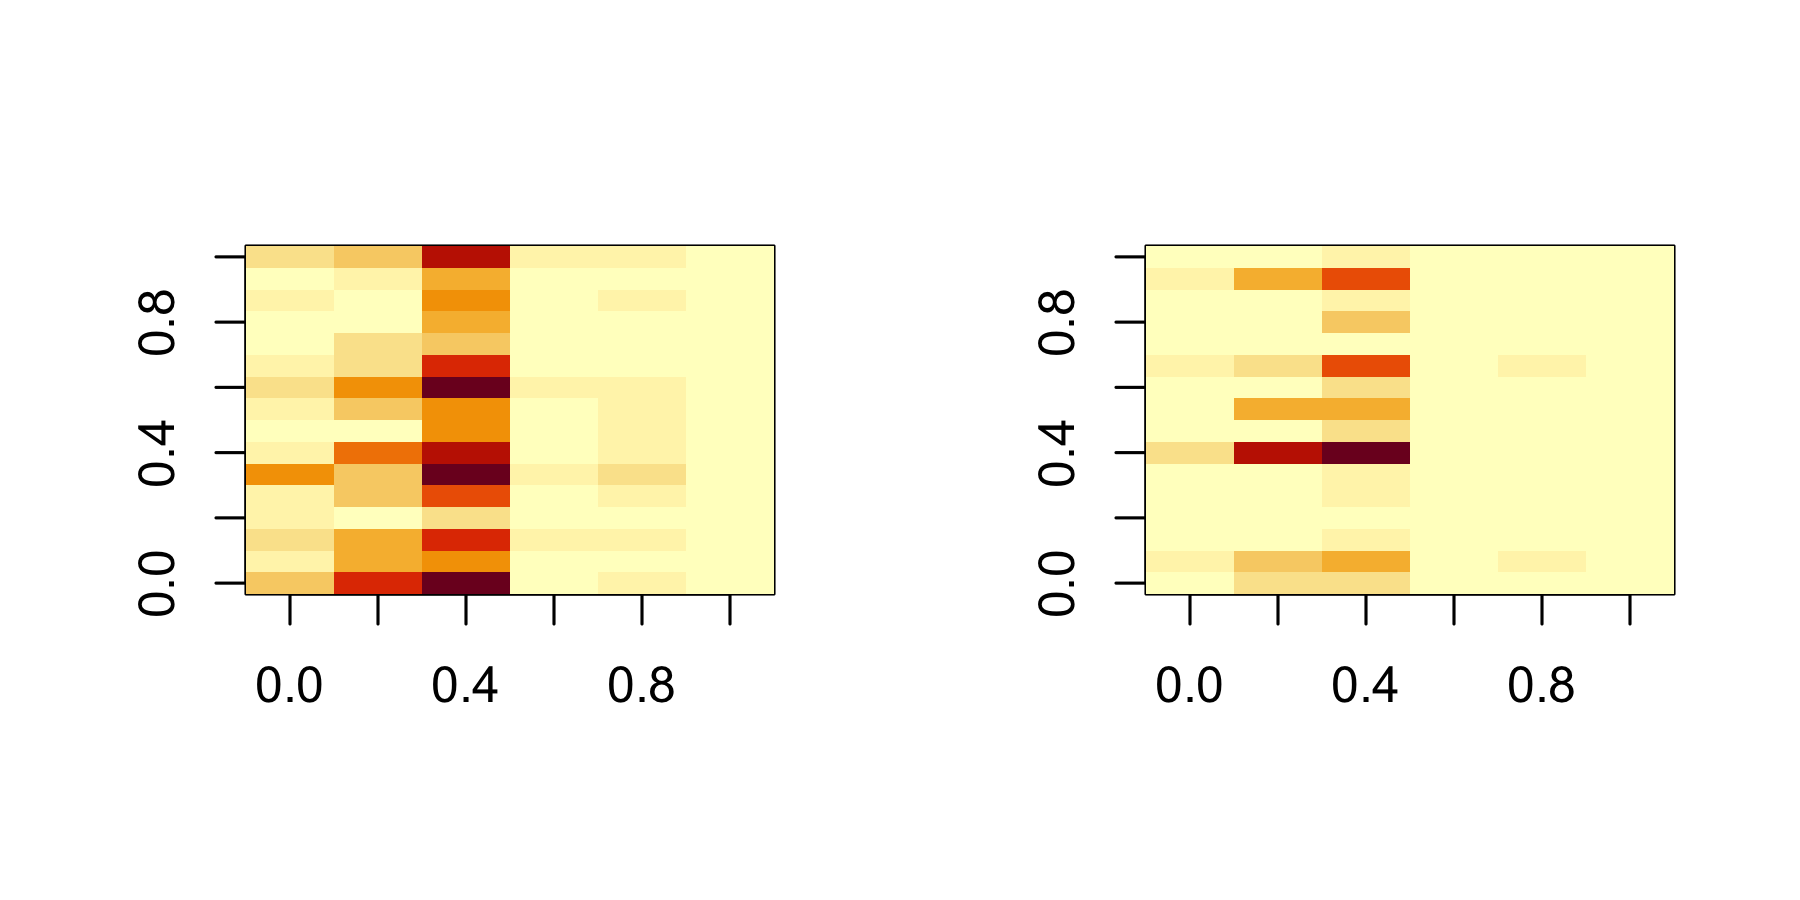
\includegraphics[width=\textwidth]{figure_roo_summary/Cervix-SCC_nucleotidesubstitution1_ROOcount_matrices_all.png}\end{minipage}\begin{minipage}{.24\textwidth}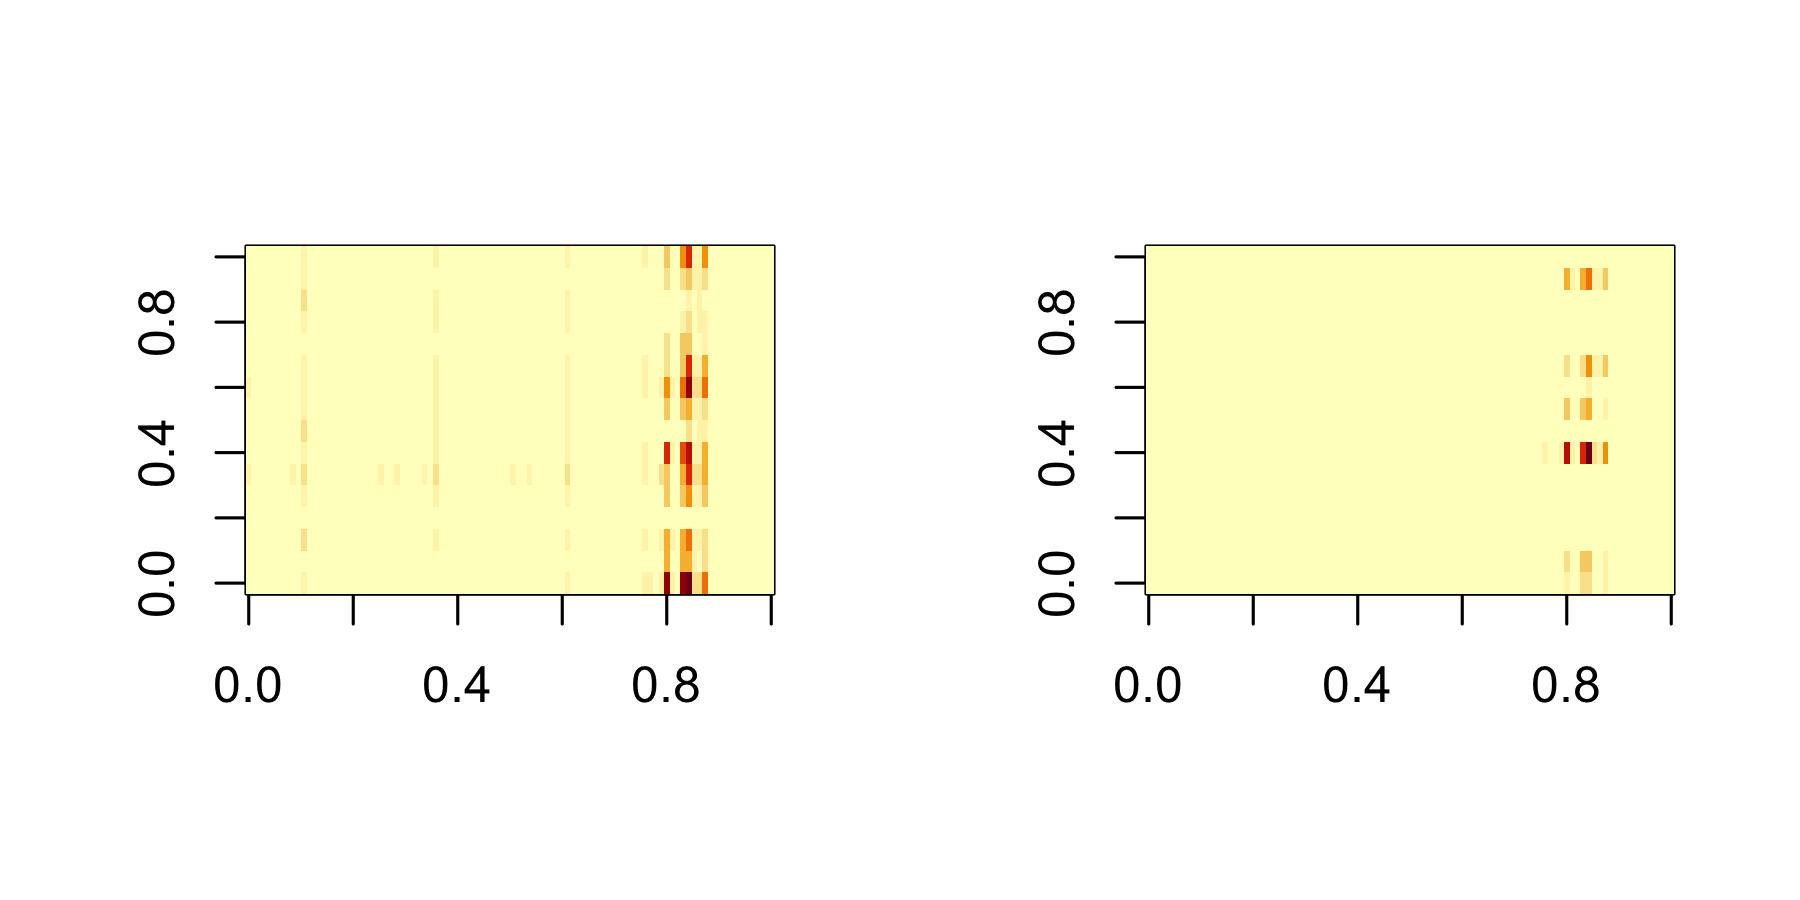
\includegraphics[width=\textwidth]{figure_roo_summary/Cervix-SCC_nucleotidesubstitution3_ROOcount_matrices_all.png}\end{minipage}\begin{minipage}{.24\textwidth}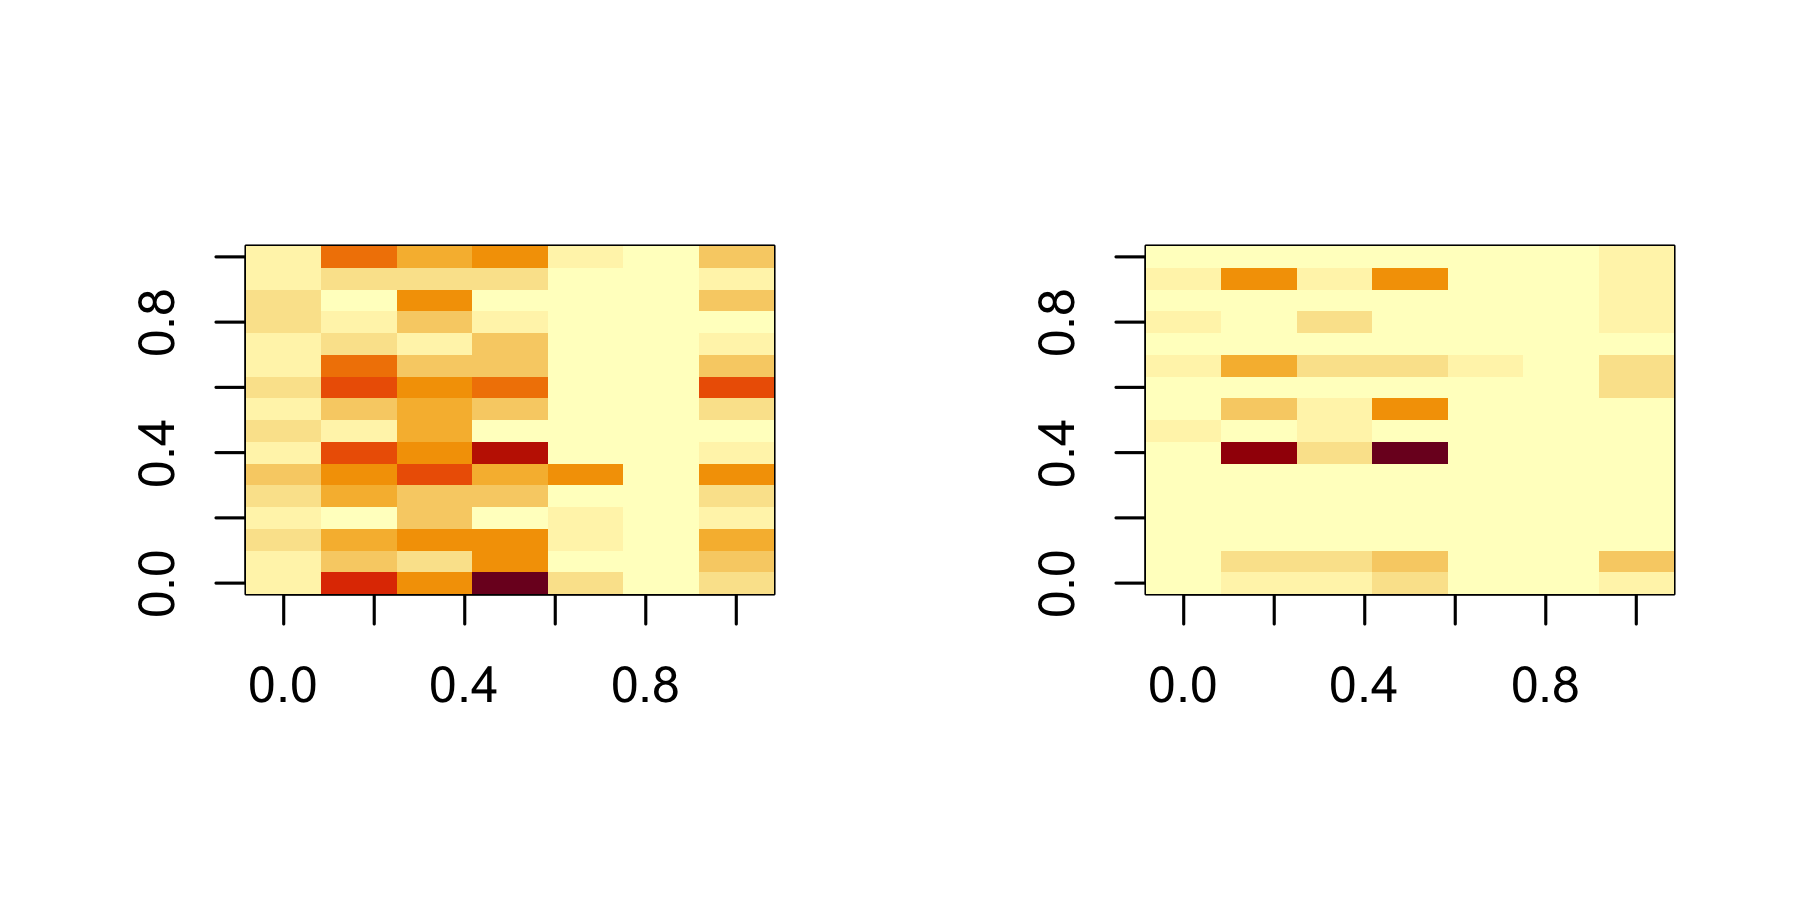
\includegraphics[width=\textwidth]{figure_roo_summary/Cervix-SCC_signatures_ROOcount_matrices_active.png}\end{minipage}\begin{minipage}{.24\textwidth}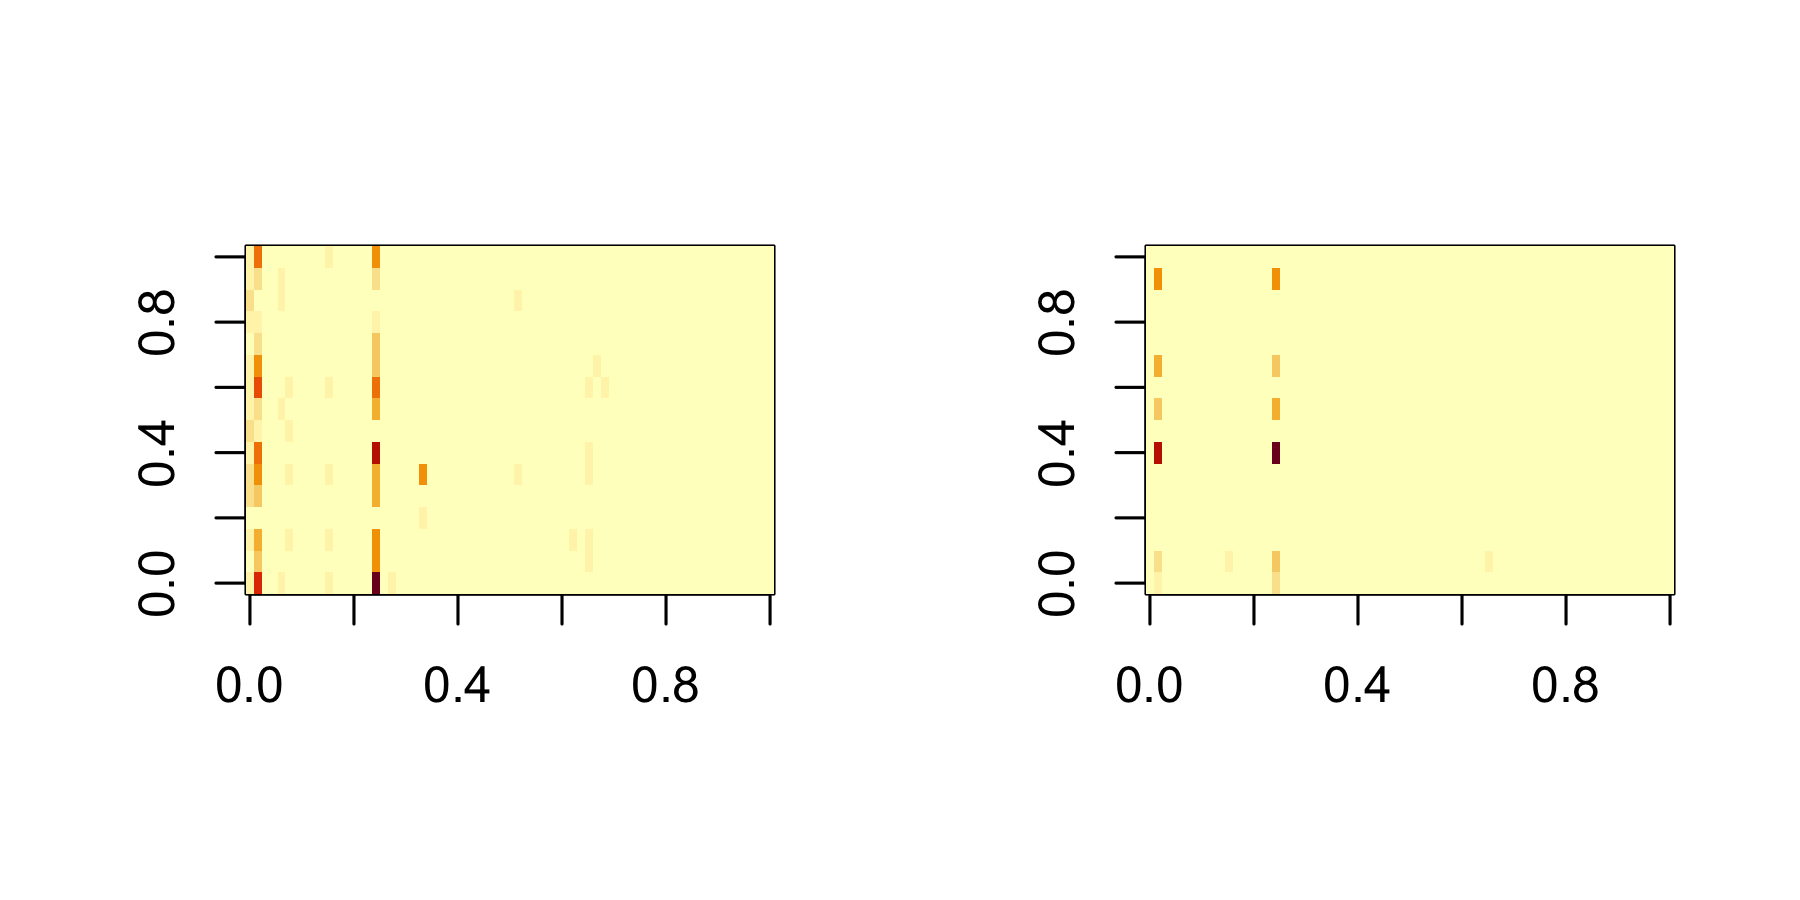
\includegraphics[width=\textwidth]{figure_roo_summary/Cervix-SCC_signatures_ROOcount_matrices_all.png}\end{minipage}\caption{Cervix-SCC}\end{figure}\begin{figure}\begin{minipage}{.24\textwidth}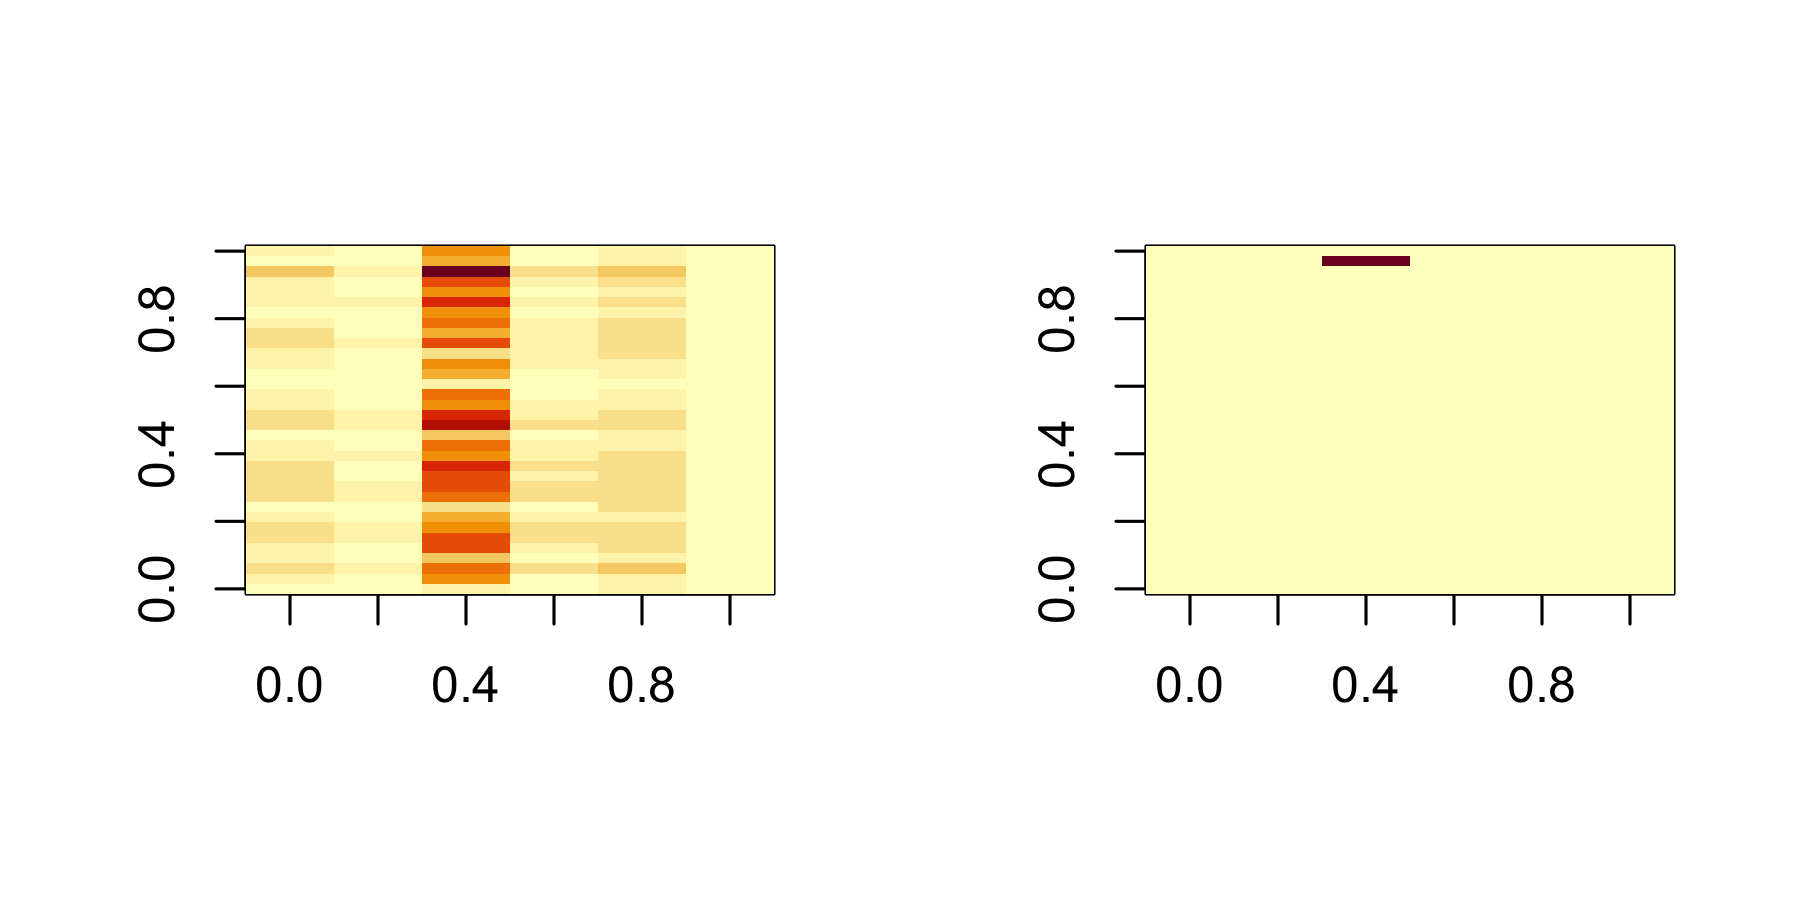
\includegraphics[width=\textwidth]{figure_roo_summary/CNS-GBM_nucleotidesubstitution1_ROOcount_matrices_all.png}\end{minipage}\begin{minipage}{.24\textwidth}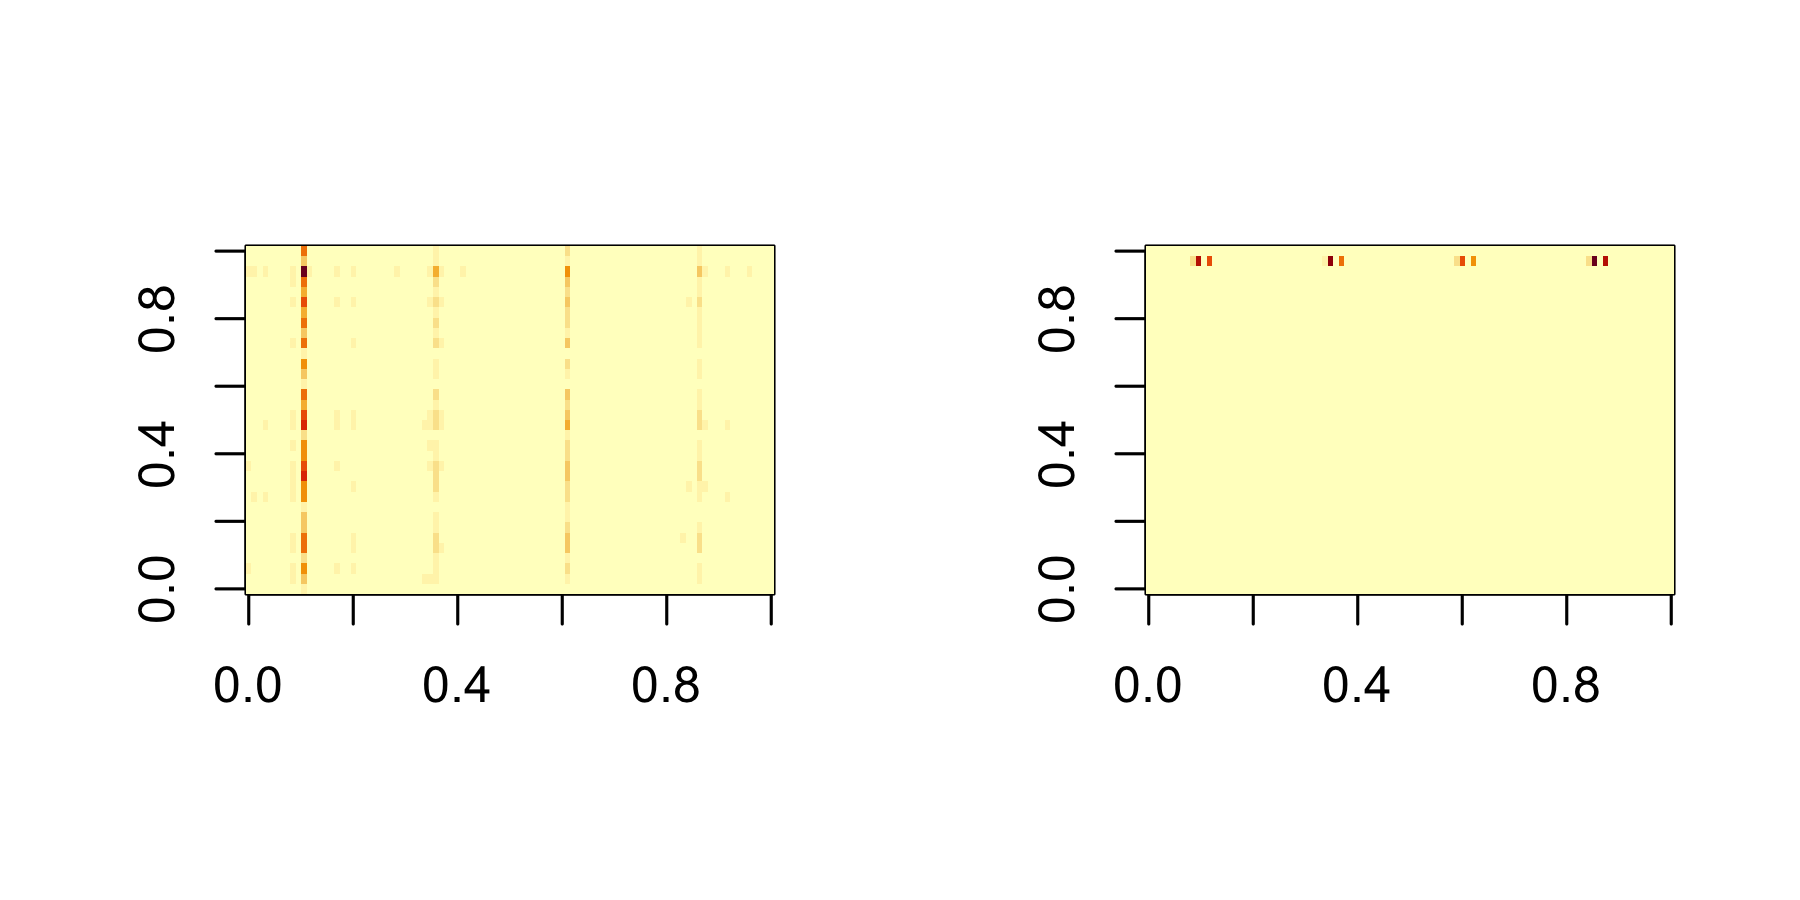
\includegraphics[width=\textwidth]{figure_roo_summary/CNS-GBM_nucleotidesubstitution3_ROOcount_matrices_all.png}\end{minipage}\begin{minipage}{.24\textwidth}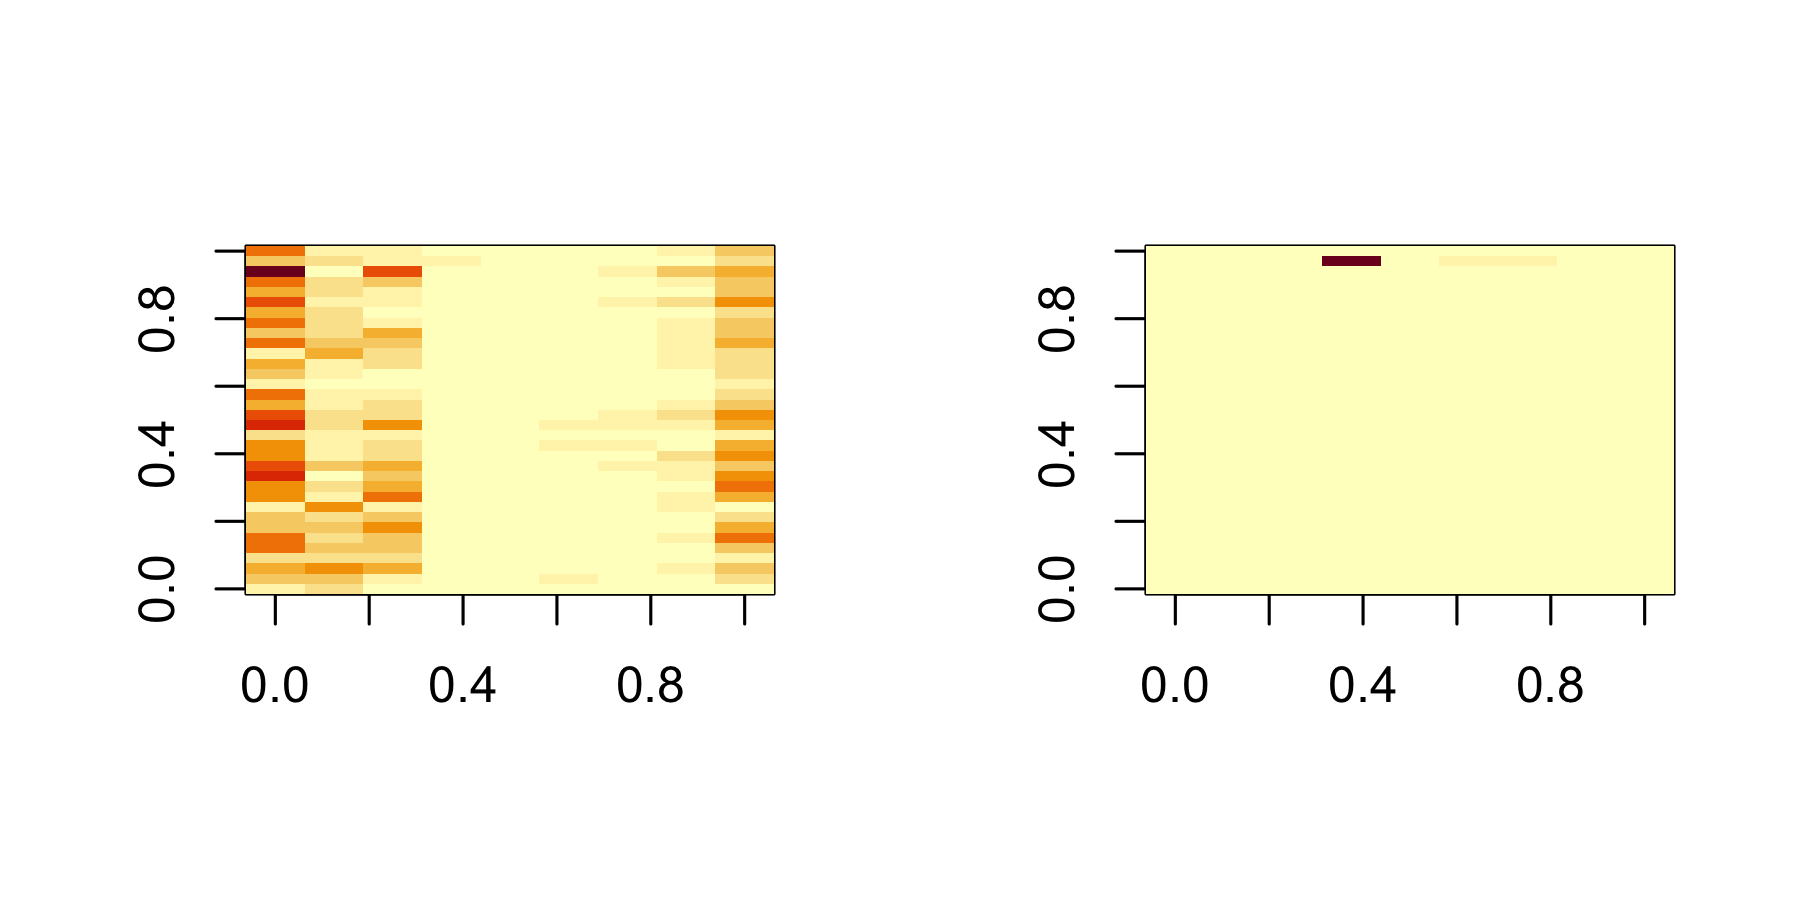
\includegraphics[width=\textwidth]{figure_roo_summary/CNS-GBM_signatures_ROOcount_matrices_active.png}\end{minipage}\begin{minipage}{.24\textwidth}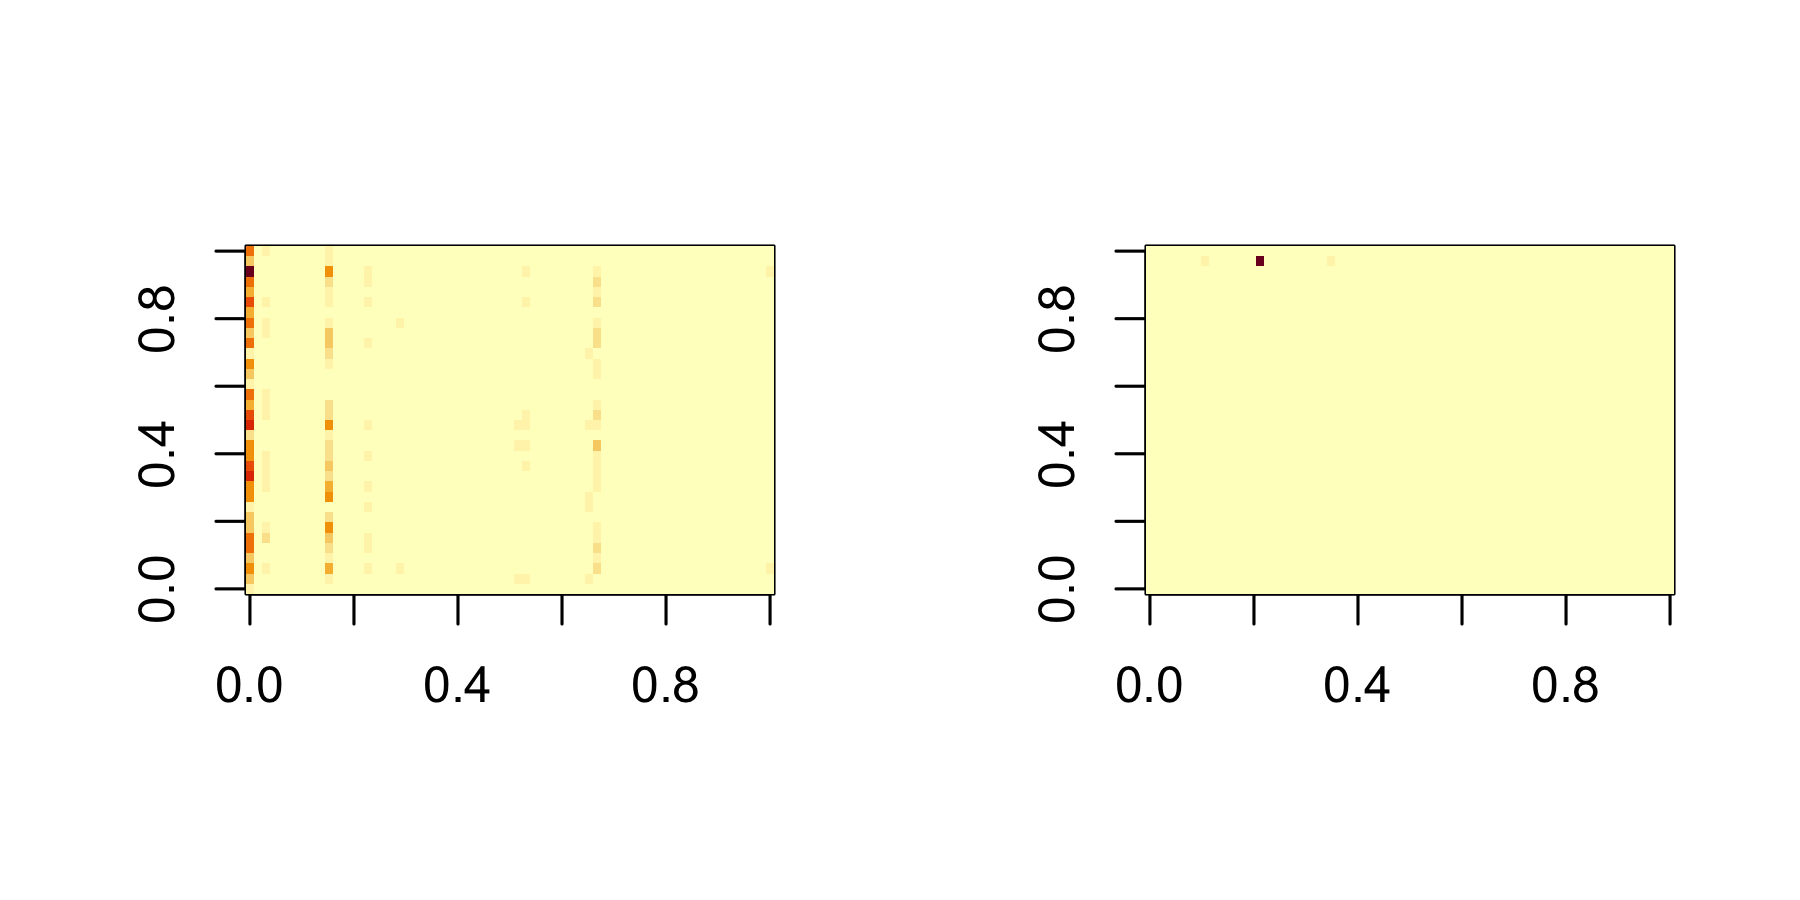
\includegraphics[width=\textwidth]{figure_roo_summary/CNS-GBM_signatures_ROOcount_matrices_all.png}\end{minipage}\caption{CNS-GBM}\end{figure}\begin{figure}\begin{minipage}{.24\textwidth}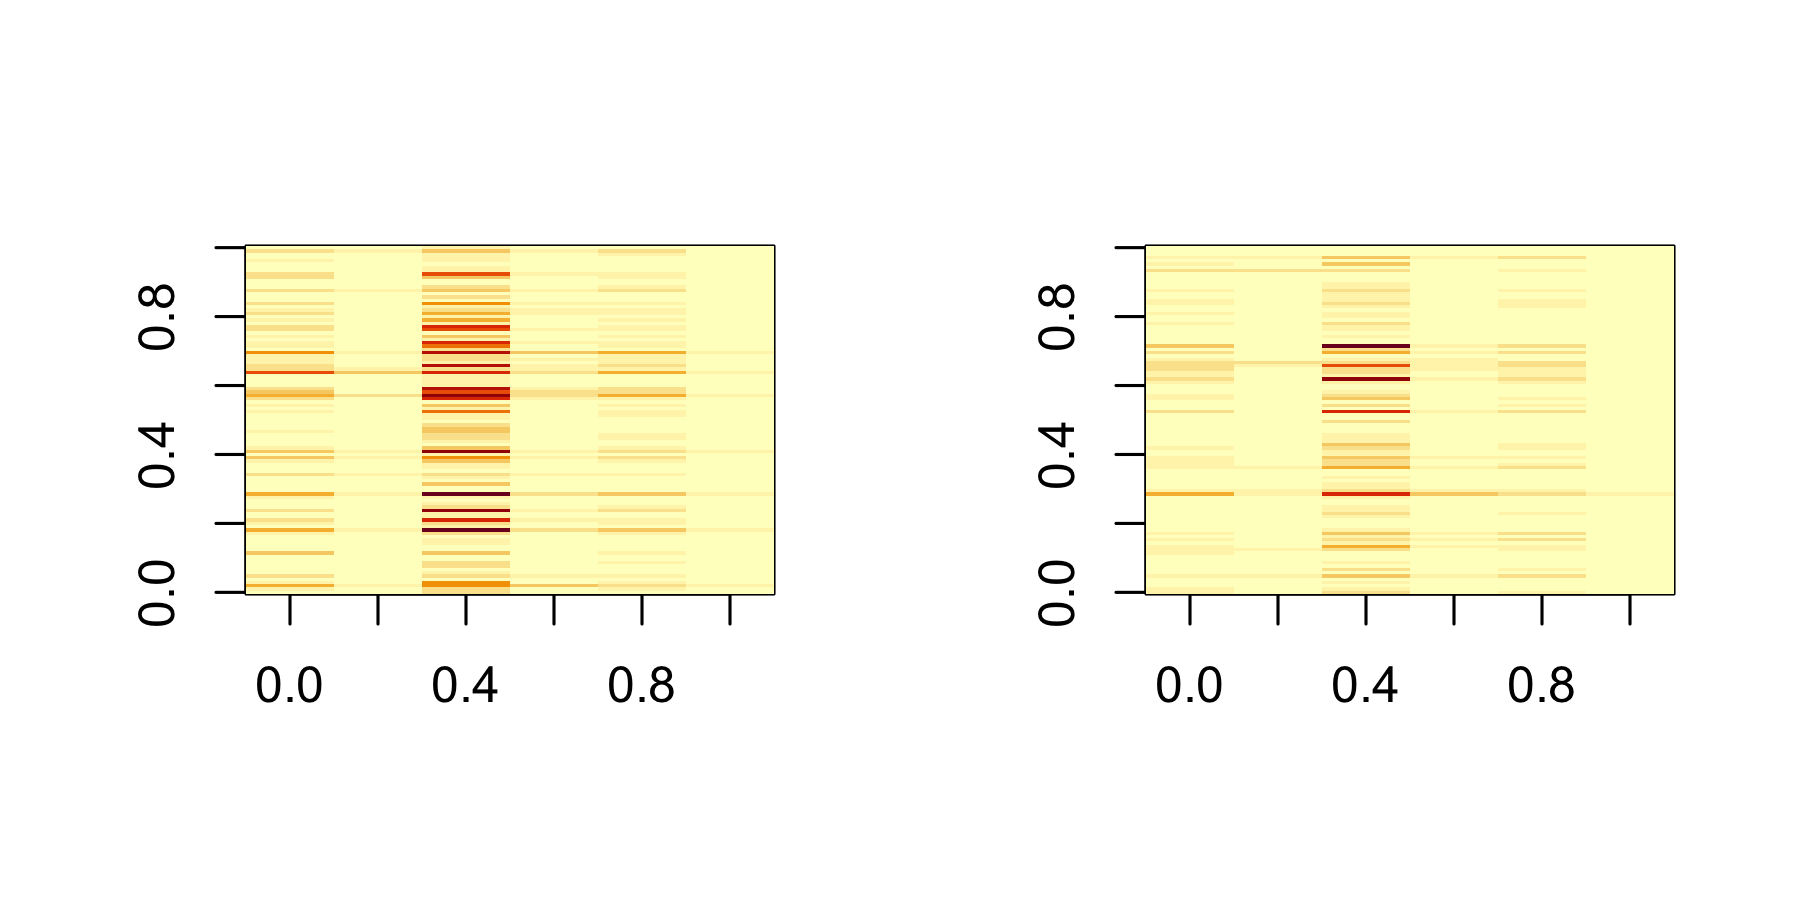
\includegraphics[width=\textwidth]{figure_roo_summary/CNS-Medullo_nucleotidesubstitution1_ROOcount_matrices_all.png}\end{minipage}\begin{minipage}{.24\textwidth}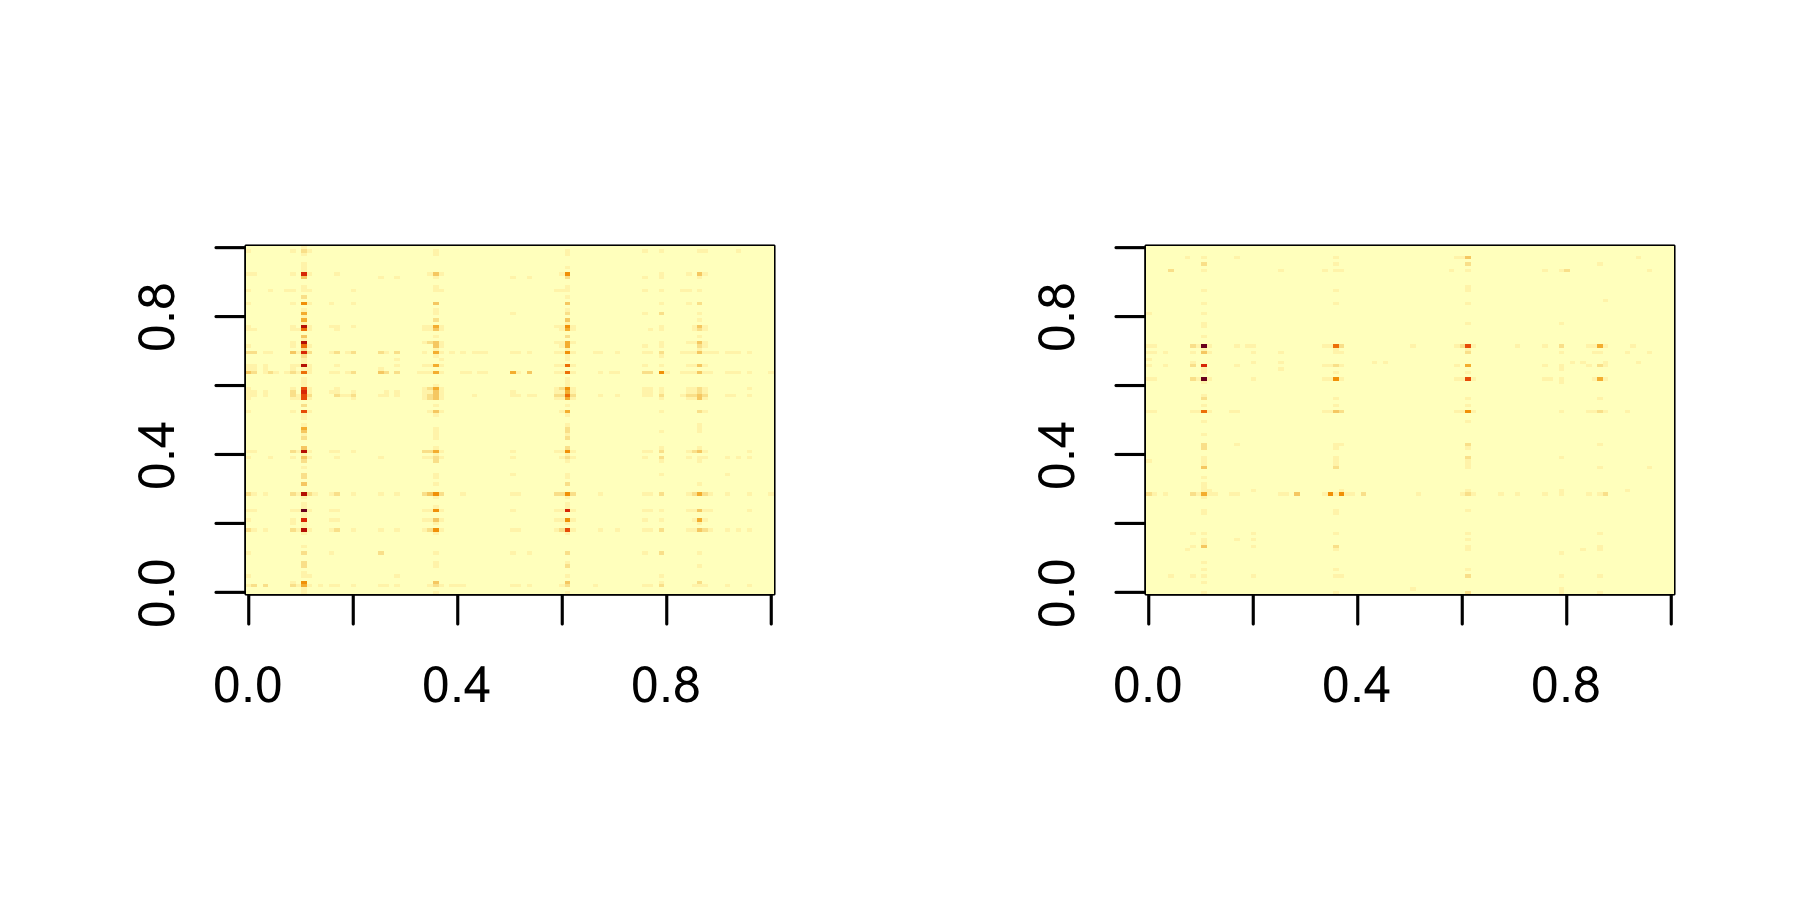
\includegraphics[width=\textwidth]{figure_roo_summary/CNS-Medullo_nucleotidesubstitution3_ROOcount_matrices_all.png}\end{minipage}\begin{minipage}{.24\textwidth}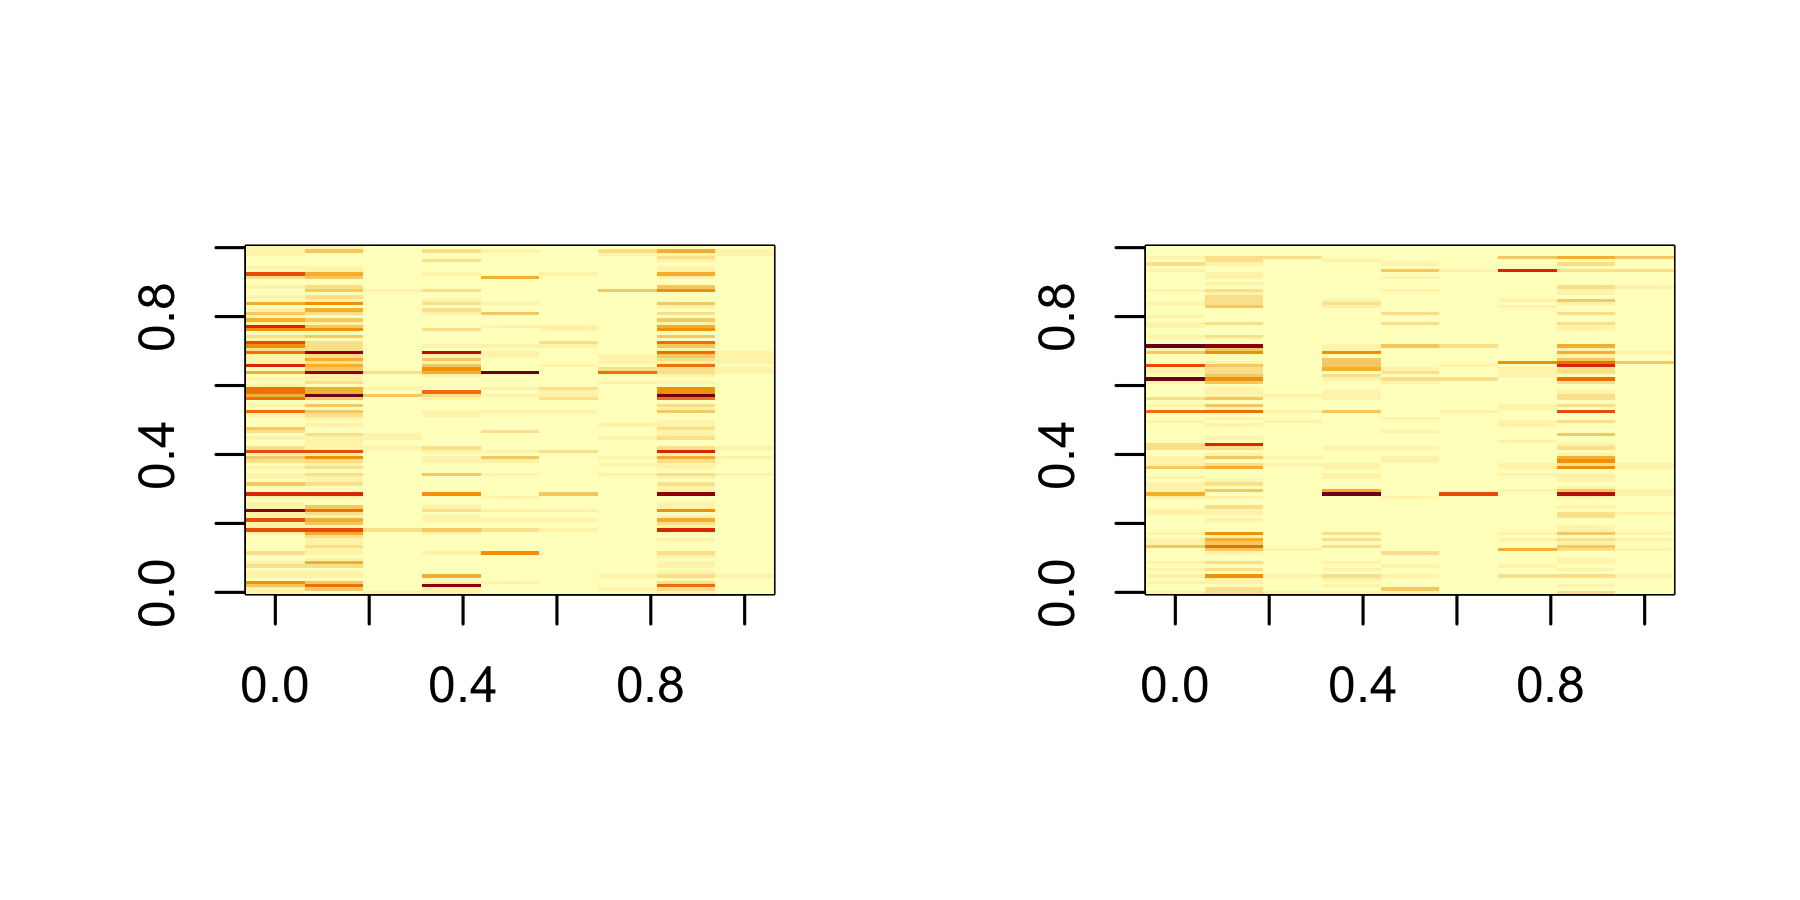
\includegraphics[width=\textwidth]{figure_roo_summary/CNS-Medullo_signatures_ROOcount_matrices_active.png}\end{minipage}\begin{minipage}{.24\textwidth}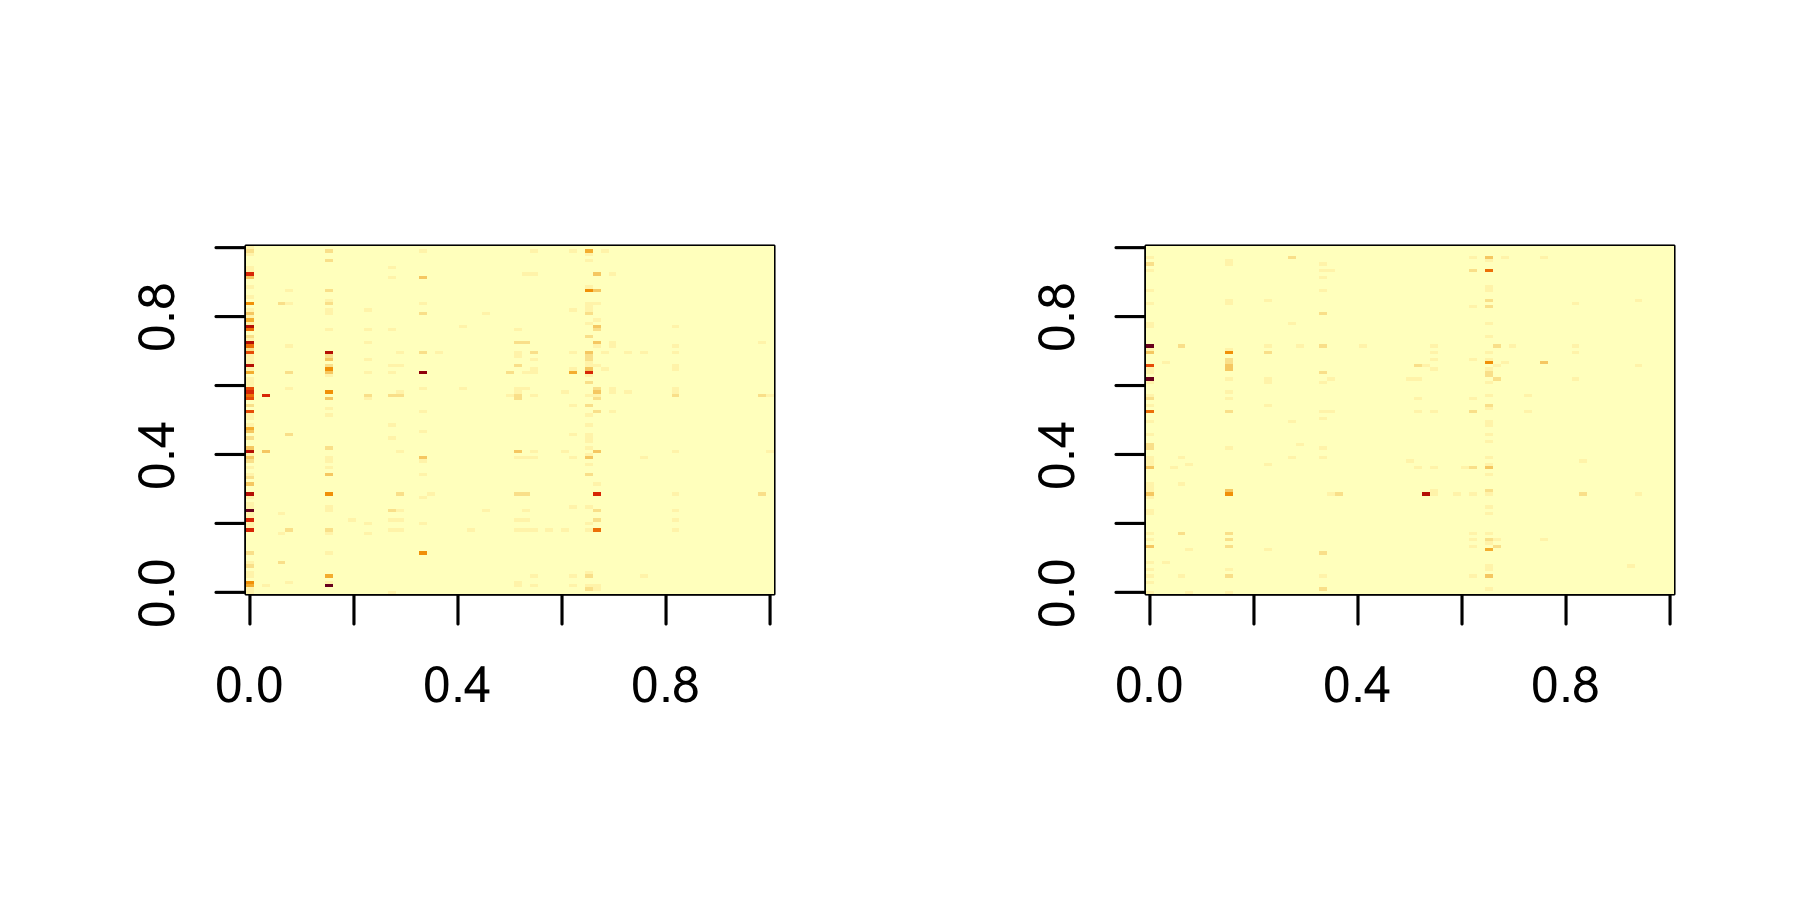
\includegraphics[width=\textwidth]{figure_roo_summary/CNS-Medullo_signatures_ROOcount_matrices_all.png}\end{minipage}\caption{CNS-Medullo}\end{figure}\begin{figure}\begin{minipage}{.24\textwidth}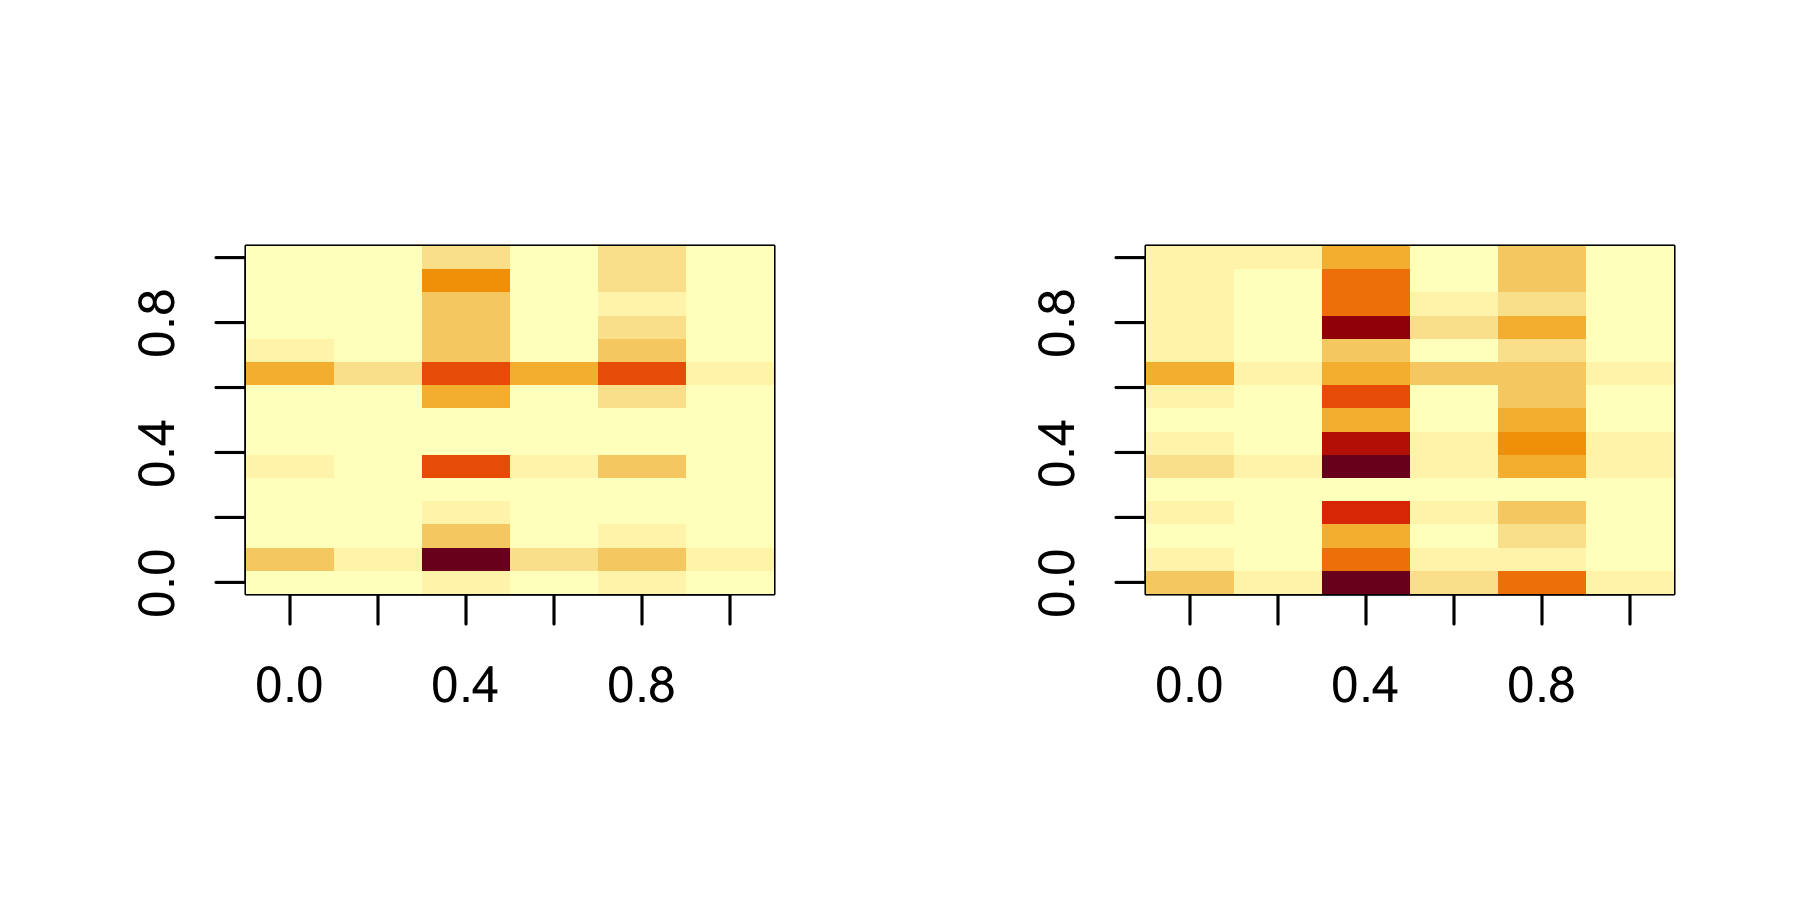
\includegraphics[width=\textwidth]{figure_roo_summary/CNS-Oligo_nucleotidesubstitution1_ROOcount_matrices_all.png}\end{minipage}\begin{minipage}{.24\textwidth}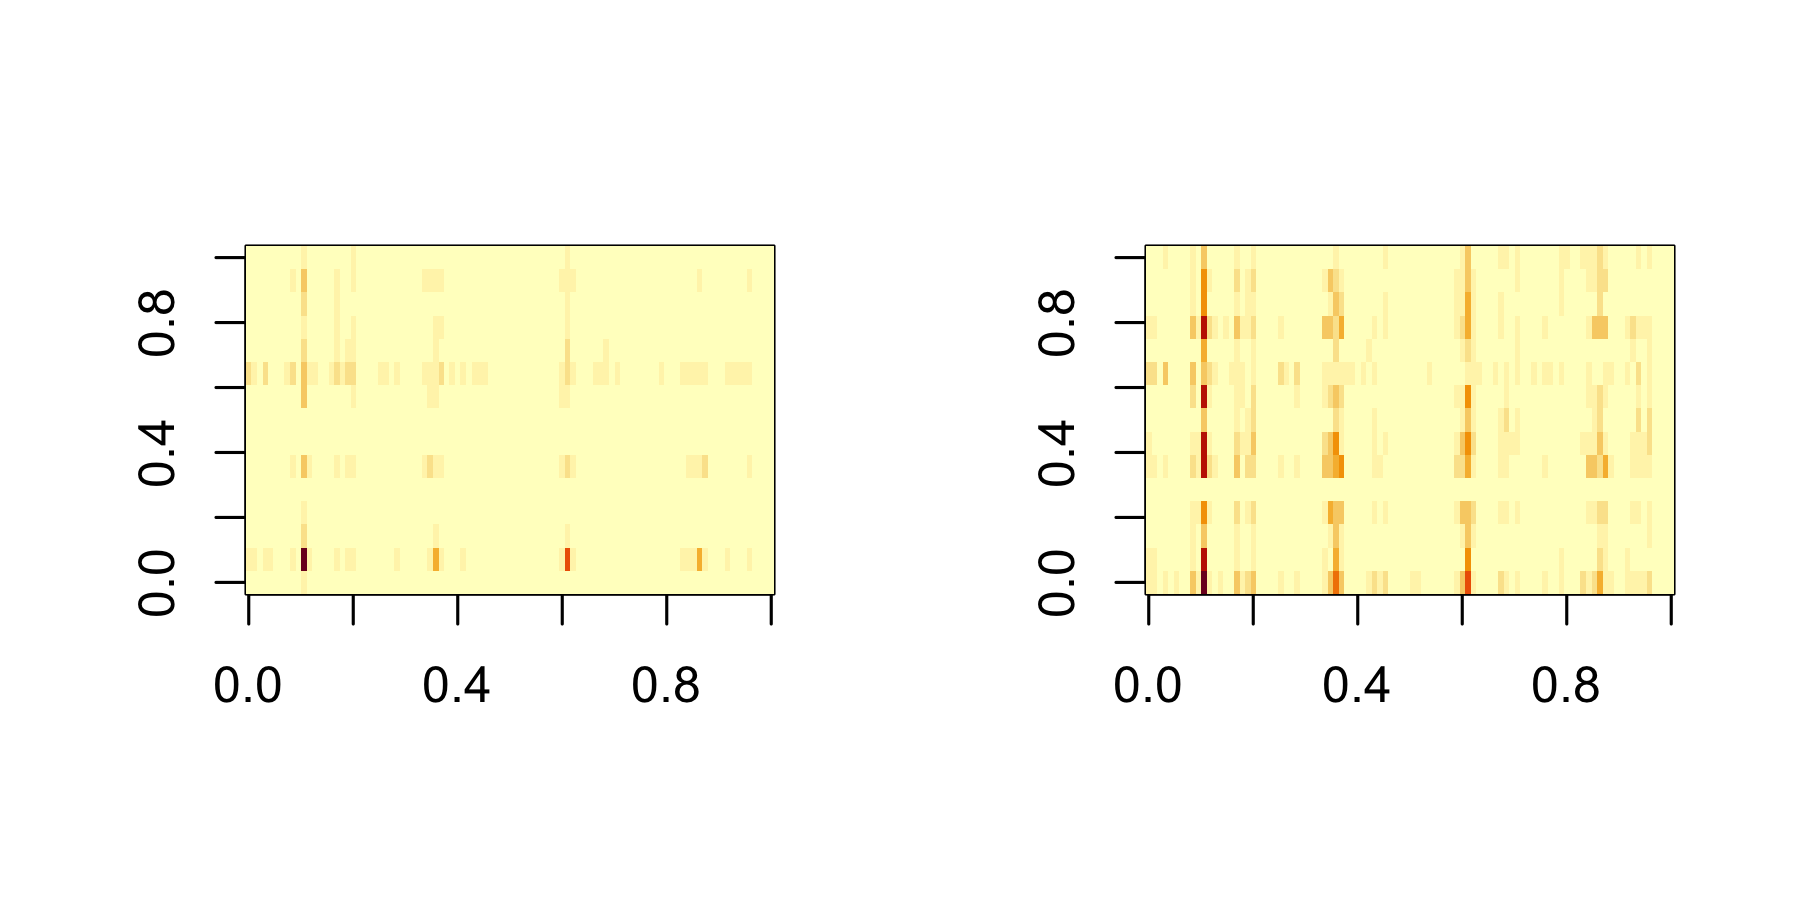
\includegraphics[width=\textwidth]{figure_roo_summary/CNS-Oligo_nucleotidesubstitution3_ROOcount_matrices_all.png}\end{minipage}\begin{minipage}{.24\textwidth}\includegraphics[width=\textwidth]{figure_roo_summary/CNS-Oligo_signatures_ROOcount_matrices_active.png}\end{minipage}\begin{minipage}{.24\textwidth}\includegraphics[width=\textwidth]{figure_roo_summary/CNS-Oligo_signatures_ROOcount_matrices_all.png}\end{minipage}\caption{CNS-Oligo}\end{figure}\begin{figure}\begin{minipage}{.24\textwidth}\includegraphics[width=\textwidth]{figure_roo_summary/CNS-PiloAstro_nucleotidesubstitution1_ROOcount_matrices_all.png}\end{minipage}\begin{minipage}{.24\textwidth}\includegraphics[width=\textwidth]{figure_roo_summary/CNS-PiloAstro_nucleotidesubstitution3_ROOcount_matrices_all.png}\end{minipage}\begin{minipage}{.24\textwidth}\includegraphics[width=\textwidth]{figure_roo_summary/CNS-PiloAstro_signatures_ROOcount_matrices_active.png}\end{minipage}\begin{minipage}{.24\textwidth}\includegraphics[width=\textwidth]{figure_roo_summary/CNS-PiloAstro_signatures_ROOcount_matrices_all.png}\end{minipage}\caption{CNS-PiloAstro}\end{figure}\begin{figure}\begin{minipage}{.24\textwidth}\includegraphics[width=\textwidth]{figure_roo_summary/ColoRect-AdenoCA_nucleotidesubstitution1_ROOcount_matrices_all.png}\end{minipage}\begin{minipage}{.24\textwidth}\includegraphics[width=\textwidth]{figure_roo_summary/ColoRect-AdenoCA_nucleotidesubstitution3_ROOcount_matrices_all.png}\end{minipage}\begin{minipage}{.24\textwidth}\includegraphics[width=\textwidth]{figure_roo_summary/ColoRect-AdenoCA_signatures_ROOcount_matrices_active.png}\end{minipage}\begin{minipage}{.24\textwidth}\includegraphics[width=\textwidth]{figure_roo_summary/ColoRect-AdenoCA_signatures_ROOcount_matrices_all.png}\end{minipage}\caption{ColoRect-AdenoCA}\end{figure}\begin{figure}\begin{minipage}{.24\textwidth}\includegraphics[width=\textwidth]{figure_roo_summary/Eso-AdenoCA_nucleotidesubstitution1_ROOcount_matrices_all.png}\end{minipage}\begin{minipage}{.24\textwidth}\includegraphics[width=\textwidth]{figure_roo_summary/Eso-AdenoCA_nucleotidesubstitution3_ROOcount_matrices_all.png}\end{minipage}\begin{minipage}{.24\textwidth}\includegraphics[width=\textwidth]{figure_roo_summary/Eso-AdenoCA_signatures_ROOcount_matrices_active.png}\end{minipage}\begin{minipage}{.24\textwidth}\includegraphics[width=\textwidth]{figure_roo_summary/Eso-AdenoCA_signatures_ROOcount_matrices_all.png}\end{minipage}\caption{Eso-AdenoCA}\end{figure}\begin{figure}\begin{minipage}{.24\textwidth}\includegraphics[width=\textwidth]{figure_roo_summary/Head-SCC_nucleotidesubstitution1_ROOcount_matrices_all.png}\end{minipage}\begin{minipage}{.24\textwidth}\includegraphics[width=\textwidth]{figure_roo_summary/Head-SCC_nucleotidesubstitution3_ROOcount_matrices_all.png}\end{minipage}\begin{minipage}{.24\textwidth}\includegraphics[width=\textwidth]{figure_roo_summary/Head-SCC_signatures_ROOcount_matrices_active.png}\end{minipage}\begin{minipage}{.24\textwidth}\includegraphics[width=\textwidth]{figure_roo_summary/Head-SCC_signatures_ROOcount_matrices_all.png}\end{minipage}\caption{Head-SCC}\end{figure}\begin{figure}\begin{minipage}{.24\textwidth}\includegraphics[width=\textwidth]{figure_roo_summary/Kidney-ChRCC_nucleotidesubstitution1_ROOcount_matrices_all.png}\end{minipage}\begin{minipage}{.24\textwidth}\includegraphics[width=\textwidth]{figure_roo_summary/Kidney-ChRCC_nucleotidesubstitution3_ROOcount_matrices_all.png}\end{minipage}\begin{minipage}{.24\textwidth}\includegraphics[width=\textwidth]{figure_roo_summary/Kidney-ChRCC_signatures_ROOcount_matrices_active.png}\end{minipage}\begin{minipage}{.24\textwidth}\includegraphics[width=\textwidth]{figure_roo_summary/Kidney-ChRCC_signatures_ROOcount_matrices_all.png}\end{minipage}\caption{Kidney-ChRCC}\end{figure}\begin{figure}\begin{minipage}{.24\textwidth}\includegraphics[width=\textwidth]{figure_roo_summary/Kidney-RCC_clearcell_nucleotidesubstitution1_ROOcount_matrices_all.png}\end{minipage}\begin{minipage}{.24\textwidth}\includegraphics[width=\textwidth]{figure_roo_summary/Kidney-RCC_clearcell_nucleotidesubstitution3_ROOcount_matrices_all.png}\end{minipage}\begin{minipage}{.24\textwidth}\includegraphics[width=\textwidth]{figure_roo_summary/Kidney-RCC_clearcell_signatures_ROOcount_matrices_active.png}\end{minipage}\begin{minipage}{.24\textwidth}\includegraphics[width=\textwidth]{figure_roo_summary/Kidney-RCC_clearcell_signatures_ROOcount_matrices_all.png}\end{minipage}\caption{Kidney-RCC.clearcell}\end{figure}\begin{figure}\begin{minipage}{.24\textwidth}\includegraphics[width=\textwidth]{figure_roo_summary/Kidney-RCC_papillary_nucleotidesubstitution1_ROOcount_matrices_all.png}\end{minipage}\begin{minipage}{.24\textwidth}\includegraphics[width=\textwidth]{figure_roo_summary/Kidney-RCC_papillary_nucleotidesubstitution3_ROOcount_matrices_all.png}\end{minipage}\begin{minipage}{.24\textwidth}\includegraphics[width=\textwidth]{figure_roo_summary/Kidney-RCC_papillary_signatures_ROOcount_matrices_active.png}\end{minipage}\begin{minipage}{.24\textwidth}\includegraphics[width=\textwidth]{figure_roo_summary/Kidney-RCC_papillary_signatures_ROOcount_matrices_all.png}\end{minipage}\caption{Kidney-RCC.papillary}\end{figure}\begin{figure}\begin{minipage}{.24\textwidth}\includegraphics[width=\textwidth]{figure_roo_summary/Liver-HCC_nucleotidesubstitution1_ROOcount_matrices_all.png}\end{minipage}\begin{minipage}{.24\textwidth}\includegraphics[width=\textwidth]{figure_roo_summary/Liver-HCC_nucleotidesubstitution3_ROOcount_matrices_all.png}\end{minipage}\begin{minipage}{.24\textwidth}\includegraphics[width=\textwidth]{figure_roo_summary/Liver-HCC_signatures_ROOcount_matrices_active.png}\end{minipage}\begin{minipage}{.24\textwidth}\includegraphics[width=\textwidth]{figure_roo_summary/Liver-HCC_signatures_ROOcount_matrices_all.png}\end{minipage}\caption{Liver-HCC}\end{figure}\begin{figure}\begin{minipage}{.24\textwidth}\includegraphics[width=\textwidth]{figure_roo_summary/Lung-AdenoCA_nucleotidesubstitution1_ROOcount_matrices_all.png}\end{minipage}\begin{minipage}{.24\textwidth}\includegraphics[width=\textwidth]{figure_roo_summary/Lung-AdenoCA_nucleotidesubstitution3_ROOcount_matrices_all.png}\end{minipage}\begin{minipage}{.24\textwidth}\includegraphics[width=\textwidth]{figure_roo_summary/Lung-AdenoCA_signatures_ROOcount_matrices_active.png}\end{minipage}\begin{minipage}{.24\textwidth}\includegraphics[width=\textwidth]{figure_roo_summary/Lung-AdenoCA_signatures_ROOcount_matrices_all.png}\end{minipage}\caption{Lung-AdenoCA}\end{figure}\begin{figure}\begin{minipage}{.24\textwidth}\includegraphics[width=\textwidth]{figure_roo_summary/Lung-SCC_nucleotidesubstitution1_ROOcount_matrices_all.png}\end{minipage}\begin{minipage}{.24\textwidth}\includegraphics[width=\textwidth]{figure_roo_summary/Lung-SCC_nucleotidesubstitution3_ROOcount_matrices_all.png}\end{minipage}\begin{minipage}{.24\textwidth}\includegraphics[width=\textwidth]{figure_roo_summary/Lung-SCC_signatures_ROOcount_matrices_active.png}\end{minipage}\begin{minipage}{.24\textwidth}\includegraphics[width=\textwidth]{figure_roo_summary/Lung-SCC_signatures_ROOcount_matrices_all.png}\end{minipage}\caption{Lung-SCC}\end{figure}\begin{figure}\begin{minipage}{.24\textwidth}\includegraphics[width=\textwidth]{figure_roo_summary/Lymph-BNHL_nucleotidesubstitution1_ROOcount_matrices_all.png}\end{minipage}\begin{minipage}{.24\textwidth}\includegraphics[width=\textwidth]{figure_roo_summary/Lymph-BNHL_nucleotidesubstitution3_ROOcount_matrices_all.png}\end{minipage}\begin{minipage}{.24\textwidth}\includegraphics[width=\textwidth]{figure_roo_summary/Lymph-BNHL_signatures_ROOcount_matrices_active.png}\end{minipage}\begin{minipage}{.24\textwidth}\includegraphics[width=\textwidth]{figure_roo_summary/Lymph-BNHL_signatures_ROOcount_matrices_all.png}\end{minipage}\caption{Lymph-BNHL}\end{figure}\begin{figure}\begin{minipage}{.24\textwidth}\includegraphics[width=\textwidth]{figure_roo_summary/Lymph-CLL_nucleotidesubstitution1_ROOcount_matrices_all.png}\end{minipage}\begin{minipage}{.24\textwidth}\includegraphics[width=\textwidth]{figure_roo_summary/Lymph-CLL_nucleotidesubstitution3_ROOcount_matrices_all.png}\end{minipage}\begin{minipage}{.24\textwidth}\includegraphics[width=\textwidth]{figure_roo_summary/Lymph-CLL_signatures_ROOcount_matrices_active.png}\end{minipage}\begin{minipage}{.24\textwidth}\includegraphics[width=\textwidth]{figure_roo_summary/Lymph-CLL_signatures_ROOcount_matrices_all.png}\end{minipage}\caption{Lymph-CLL}\end{figure}\begin{figure}\begin{minipage}{.24\textwidth}\includegraphics[width=\textwidth]{figure_roo_summary/Myeloid-AML_nucleotidesubstitution1_ROOcount_matrices_all.png}\end{minipage}\begin{minipage}{.24\textwidth}\includegraphics[width=\textwidth]{figure_roo_summary/Myeloid-AML_nucleotidesubstitution3_ROOcount_matrices_all.png}\end{minipage}\begin{minipage}{.24\textwidth}\includegraphics[width=\textwidth]{figure_roo_summary/Myeloid-AML_signatures_ROOcount_matrices_active.png}\end{minipage}\begin{minipage}{.24\textwidth}\includegraphics[width=\textwidth]{figure_roo_summary/Myeloid-AML_signatures_ROOcount_matrices_all.png}\end{minipage}\caption{Myeloid-AML}\end{figure}\begin{figure}\begin{minipage}{.24\textwidth}\includegraphics[width=\textwidth]{figure_roo_summary/Myeloid-MPN_nucleotidesubstitution1_ROOcount_matrices_all.png}\end{minipage}\begin{minipage}{.24\textwidth}\includegraphics[width=\textwidth]{figure_roo_summary/Myeloid-MPN_nucleotidesubstitution3_ROOcount_matrices_all.png}\end{minipage}\begin{minipage}{.24\textwidth}\includegraphics[width=\textwidth]{figure_roo_summary/Myeloid-MPN_signatures_ROOcount_matrices_active.png}\end{minipage}\begin{minipage}{.24\textwidth}\includegraphics[width=\textwidth]{figure_roo_summary/Myeloid-MPN_signatures_ROOcount_matrices_all.png}\end{minipage}\caption{Myeloid-MPN}\end{figure}\begin{figure}\begin{minipage}{.24\textwidth}\includegraphics[width=\textwidth]{figure_roo_summary/Ovary-AdenoCA_nucleotidesubstitution1_ROOcount_matrices_all.png}\end{minipage}\begin{minipage}{.24\textwidth}\includegraphics[width=\textwidth]{figure_roo_summary/Ovary-AdenoCA_nucleotidesubstitution3_ROOcount_matrices_all.png}\end{minipage}\begin{minipage}{.24\textwidth}\includegraphics[width=\textwidth]{figure_roo_summary/Ovary-AdenoCA_signatures_ROOcount_matrices_active.png}\end{minipage}\begin{minipage}{.24\textwidth}\includegraphics[width=\textwidth]{figure_roo_summary/Ovary-AdenoCA_signatures_ROOcount_matrices_all.png}\end{minipage}\caption{Ovary-AdenoCA}\end{figure}\begin{figure}\begin{minipage}{.24\textwidth}\includegraphics[width=\textwidth]{figure_roo_summary/Panc-AdenoCA_nucleotidesubstitution1_ROOcount_matrices_all.png}\end{minipage}\begin{minipage}{.24\textwidth}\includegraphics[width=\textwidth]{figure_roo_summary/Panc-AdenoCA_nucleotidesubstitution3_ROOcount_matrices_all.png}\end{minipage}\begin{minipage}{.24\textwidth}\includegraphics[width=\textwidth]{figure_roo_summary/Panc-AdenoCA_signatures_ROOcount_matrices_active.png}\end{minipage}\begin{minipage}{.24\textwidth}\includegraphics[width=\textwidth]{figure_roo_summary/Panc-AdenoCA_signatures_ROOcount_matrices_all.png}\end{minipage}\caption{Panc-AdenoCA}\end{figure}\begin{figure}\begin{minipage}{.24\textwidth}\includegraphics[width=\textwidth]{figure_roo_summary/Panc-Endocrine_nucleotidesubstitution1_ROOcount_matrices_all.png}\end{minipage}\begin{minipage}{.24\textwidth}\includegraphics[width=\textwidth]{figure_roo_summary/Panc-Endocrine_nucleotidesubstitution3_ROOcount_matrices_all.png}\end{minipage}\begin{minipage}{.24\textwidth}\includegraphics[width=\textwidth]{figure_roo_summary/Panc-Endocrine_signatures_ROOcount_matrices_active.png}\end{minipage}\begin{minipage}{.24\textwidth}\includegraphics[width=\textwidth]{figure_roo_summary/Panc-Endocrine_signatures_ROOcount_matrices_all.png}\end{minipage}\caption{Panc-Endocrine}\end{figure}\begin{figure}\begin{minipage}{.24\textwidth}\includegraphics[width=\textwidth]{figure_roo_summary/Prost-AdenoCA_nucleotidesubstitution1_ROOcount_matrices_all.png}\end{minipage}\begin{minipage}{.24\textwidth}\includegraphics[width=\textwidth]{figure_roo_summary/Prost-AdenoCA_nucleotidesubstitution3_ROOcount_matrices_all.png}\end{minipage}\begin{minipage}{.24\textwidth}\includegraphics[width=\textwidth]{figure_roo_summary/Prost-AdenoCA_signatures_ROOcount_matrices_active.png}\end{minipage}\begin{minipage}{.24\textwidth}\includegraphics[width=\textwidth]{figure_roo_summary/Prost-AdenoCA_signatures_ROOcount_matrices_all.png}\end{minipage}\caption{Prost-AdenoCA}\end{figure}\begin{figure}\begin{minipage}{.24\textwidth}\includegraphics[width=\textwidth]{figure_roo_summary/Skin-Melanoma_acral_nucleotidesubstitution1_ROOcount_matrices_all.png}\end{minipage}\begin{minipage}{.24\textwidth}\includegraphics[width=\textwidth]{figure_roo_summary/Skin-Melanoma_acral_nucleotidesubstitution3_ROOcount_matrices_all.png}\end{minipage}\begin{minipage}{.24\textwidth}\includegraphics[width=\textwidth]{figure_roo_summary/Skin-Melanoma_acral_signatures_ROOcount_matrices_active.png}\end{minipage}\begin{minipage}{.24\textwidth}\includegraphics[width=\textwidth]{figure_roo_summary/Skin-Melanoma_acral_signatures_ROOcount_matrices_all.png}\end{minipage}\caption{Skin-Melanoma.acral}\end{figure}\begin{figure}\begin{minipage}{.24\textwidth}\includegraphics[width=\textwidth]{figure_roo_summary/Skin-Melanoma_cutaneous_nucleotidesubstitution1_ROOcount_matrices_all.png}\end{minipage}\begin{minipage}{.24\textwidth}\includegraphics[width=\textwidth]{figure_roo_summary/Skin-Melanoma_cutaneous_nucleotidesubstitution3_ROOcount_matrices_all.png}\end{minipage}\begin{minipage}{.24\textwidth}\includegraphics[width=\textwidth]{figure_roo_summary/Skin-Melanoma_cutaneous_signatures_ROOcount_matrices_active.png}\end{minipage}\begin{minipage}{.24\textwidth}\includegraphics[width=\textwidth]{figure_roo_summary/Skin-Melanoma_cutaneous_signatures_ROOcount_matrices_all.png}\end{minipage}\caption{Skin-Melanoma.cutaneous}\end{figure}\begin{figure}\begin{minipage}{.24\textwidth}\includegraphics[width=\textwidth]{figure_roo_summary/Skin-Melanoma_mucosal_nucleotidesubstitution1_ROOcount_matrices_all.png}\end{minipage}\begin{minipage}{.24\textwidth}\includegraphics[width=\textwidth]{figure_roo_summary/Skin-Melanoma_mucosal_nucleotidesubstitution3_ROOcount_matrices_all.png}\end{minipage}\begin{minipage}{.24\textwidth}\includegraphics[width=\textwidth]{figure_roo_summary/Skin-Melanoma_mucosal_signatures_ROOcount_matrices_active.png}\end{minipage}\begin{minipage}{.24\textwidth}\includegraphics[width=\textwidth]{figure_roo_summary/Skin-Melanoma_mucosal_signatures_ROOcount_matrices_all.png}\end{minipage}\caption{Skin-Melanoma.mucosal}\end{figure}\begin{figure}\begin{minipage}{.24\textwidth}\includegraphics[width=\textwidth]{figure_roo_summary/SoftTissue-Leiomyo_nucleotidesubstitution1_ROOcount_matrices_all.png}\end{minipage}\begin{minipage}{.24\textwidth}\includegraphics[width=\textwidth]{figure_roo_summary/SoftTissue-Leiomyo_nucleotidesubstitution3_ROOcount_matrices_all.png}\end{minipage}\begin{minipage}{.24\textwidth}\includegraphics[width=\textwidth]{figure_roo_summary/SoftTissue-Leiomyo_signatures_ROOcount_matrices_active.png}\end{minipage}\begin{minipage}{.24\textwidth}\includegraphics[width=\textwidth]{figure_roo_summary/SoftTissue-Leiomyo_signatures_ROOcount_matrices_all.png}\end{minipage}\caption{SoftTissue-Leiomyo}\end{figure}\begin{figure}\begin{minipage}{.24\textwidth}\includegraphics[width=\textwidth]{figure_roo_summary/SoftTissue-Liposarc_nucleotidesubstitution1_ROOcount_matrices_all.png}\end{minipage}\begin{minipage}{.24\textwidth}\includegraphics[width=\textwidth]{figure_roo_summary/SoftTissue-Liposarc_nucleotidesubstitution3_ROOcount_matrices_all.png}\end{minipage}\begin{minipage}{.24\textwidth}\includegraphics[width=\textwidth]{figure_roo_summary/SoftTissue-Liposarc_signatures_ROOcount_matrices_active.png}\end{minipage}\begin{minipage}{.24\textwidth}\includegraphics[width=\textwidth]{figure_roo_summary/SoftTissue-Liposarc_signatures_ROOcount_matrices_all.png}\end{minipage}\caption{SoftTissue-Liposarc}\end{figure}\begin{figure}\begin{minipage}{.24\textwidth}\includegraphics[width=\textwidth]{figure_roo_summary/Stomach-AdenoCA_nucleotidesubstitution1_ROOcount_matrices_all.png}\end{minipage}\begin{minipage}{.24\textwidth}\includegraphics[width=\textwidth]{figure_roo_summary/Stomach-AdenoCA_nucleotidesubstitution3_ROOcount_matrices_all.png}\end{minipage}\begin{minipage}{.24\textwidth}\includegraphics[width=\textwidth]{figure_roo_summary/Stomach-AdenoCA_signatures_ROOcount_matrices_active.png}\end{minipage}\begin{minipage}{.24\textwidth}\includegraphics[width=\textwidth]{figure_roo_summary/Stomach-AdenoCA_signatures_ROOcount_matrices_all.png}\end{minipage}\caption{Stomach-AdenoCA}\end{figure}\begin{figure}\begin{minipage}{.24\textwidth}\includegraphics[width=\textwidth]{figure_roo_summary/Thy-AdenoCA_nucleotidesubstitution1_ROOcount_matrices_all.png}\end{minipage}\begin{minipage}{.24\textwidth}\includegraphics[width=\textwidth]{figure_roo_summary/Thy-AdenoCA_nucleotidesubstitution3_ROOcount_matrices_all.png}\end{minipage}\begin{minipage}{.24\textwidth}\includegraphics[width=\textwidth]{figure_roo_summary/Thy-AdenoCA_signatures_ROOcount_matrices_active.png}\end{minipage}\begin{minipage}{.24\textwidth}\includegraphics[width=\textwidth]{figure_roo_summary/Thy-AdenoCA_signatures_ROOcount_matrices_all.png}\end{minipage}\caption{Thy-AdenoCA}\end{figure}\begin{figure}\begin{minipage}{.24\textwidth}\includegraphics[width=\textwidth]{figure_roo_summary/Uterus-AdenoCA_nucleotidesubstitution1_ROOcount_matrices_all.png}\end{minipage}\begin{minipage}{.24\textwidth}\includegraphics[width=\textwidth]{figure_roo_summary/Uterus-AdenoCA_nucleotidesubstitution3_ROOcount_matrices_all.png}\end{minipage}\begin{minipage}{.24\textwidth}\includegraphics[width=\textwidth]{figure_roo_summary/Uterus-AdenoCA_signatures_ROOcount_matrices_active.png}\end{minipage}\begin{minipage}{.24\textwidth}\includegraphics[width=\textwidth]{figure_roo_summary/Uterus-AdenoCA_signatures_ROOcount_matrices_all.png}\end{minipage}\caption{Uterus-AdenoCA}\end{figure}\end{document}
